\documentclass[main.tex]{subfiles}                                              
\begin{document}

\section{曲线和曲面的点反演与投影}

在本章中，我们将讨论在实现 NURBS 几何时相当基础的各种主题。

给定一个点 \(\mathbf{P} = \left( {x,y,z}\right)\) ，假设它位于 NURBS 曲线 \(\mathbf{C}\left( u\right)\) 上，该曲线的度数为 \(p\) ，点反演是寻找相应参数 \(\bar{u}\) 的问题，使得 \(\mathbf{C}\left( \bar{u}\right)  = \mathbf{P}\) 。理论上，如果满足 \(p \leq  4\) ，点反演可以以封闭形式解决。步骤如下:

1. 使用强凸包性质 (P4.10)，确定 \(\mathbf{C}\left( u\right)\) 的哪些跨度可能包含 \(\mathbf{P}\) ；

2. 使用节点插入或细化，提取候选跨度并将其转换为幂基形式；

3. 每个跨度导致一个未知数的三个多项式方程；如果这三个方程有一个共同解，则 \(\mathbf{P}\) 位于曲线的该段上。

作为步骤 3 的一个例子，假设 \(p = 2\) 。然后，跨度 \(\mathbf{r}\left( u\right)\) 由向量函数给出(在四维空间中):

\[
\mathbf{r}\left( u\right)  = {\mathbf{a}}_{0}^{w} + {\mathbf{a}}_{1}^{w}u + {\mathbf{a}}_{2}^{w}{u}^{2} \tag{6.1}
\]

设 \({\mathbf{a}}_{i}^{w} = \left( {{w}_{i}{x}_{i},{w}_{i}{y}_{i},{w}_{i}{z}_{i},{w}_{i}}\right)\) 。将方程 (6.1) 投影到三维空间并设其等于 \(\mathbf{P} = \left( {x,y,z}\right)\) ，我们得到

\[
\frac{{w}_{2}{x}_{2}{u}^{2} + {w}_{1}{x}_{1}u + {w}_{0}{x}_{0}}{{w}_{2}{u}^{2} + {w}_{1}u + {w}_{0}} = x
\]

\[
\frac{{w}_{2}{y}_{2}{u}^{2} + {w}_{1}{y}_{1}u + {w}_{0}{y}_{0}}{{w}_{2}{u}^{2} + {w}_{1}u + {w}_{0}} = y
\]

\[
\frac{{w}_{2}{z}_{2}{u}^{2} + {w}_{1}{z}_{1}u + {w}_{0}{z}_{0}}{{w}_{2}{u}^{2} + {w}_{1}u + {w}_{0}} = z
\]

这导致 \({w}_{2}\left( {{x}_{2} - x}\right) {u}^{2} + {w}_{1}\left( {{x}_{1} - x}\right) u + {w}_{0}\left( {{x}_{0} - x}\right)  = 0\)

\[
{w}_{2}\left( {{y}_{2} - y}\right) {u}^{2} + {w}_{1}\left( {{y}_{1} - y}\right) u + {w}_{0}\left( {{y}_{0} - y}\right)  = 0
\]

\[
{w}_{2}\left( {{z}_{2} - z}\right) {u}^{2} + {w}_{1}\left( {{z}_{1} - z}\right) u + {w}_{0}\left( {{z}_{0} - z}\right)  = 0 \tag{6.2}
\]

该方法有其缺点，例如:

\begin{itemize}
\item 方程 (6.2) 对于 \(p > 4\) 不能以封闭形式求解，并且 \(p = 3\) 和 \(p = 4\) 的解在计算机上并非没有问题；
\end{itemize}

\begin{itemize}
\item 存在数值容差问题，例如，不能期望方程 (6.2) 的三个解完全相等；但何时应将它们视为相等？当点 \(\mathbf{P}\) 并不精确位于曲线上时(这种情况很常见)，问题会加剧；
\end{itemize}

\begin{itemize}
\item 之前解决方案的软件实现相当复杂。
\end{itemize}

一种更简单且完全足够的方法是使用牛顿迭代来最小化 \(\mathbf{P}\) 和 \(\mathbf{C}\left( u\right)\) 之间的距离(见图 6.1a 和 6.1b)。如果最小距离小于指定的容差 \({\epsilon }_{1}\) ，则认为 \(\mathbf{P}\) 在曲线上。这有效地解决了点投影到曲线的更一般问题。为了获得牛顿迭代的起始值 \({u}_{0}\) :

\begin{itemize}
\item 如果已知该点位于曲线上(在容差范围内)，则使用强凸包性质来确定候选跨度；如果这是一个更一般的点投影问题，则选择所有跨度作为候选；
\end{itemize}

\begin{itemize}
\item 在每个候选跨度上以均匀间隔的参数值评估曲线点 \(n\) ，并计算每个点与 \(\mathbf{P}\) 的距离。选择 \({u}_{0}\) 作为使点最接近 \(\mathbf{P}\) 的值；数字 \(n\) 通常通过某种启发式方法选择。我们强调，良好的起始值对于实现可靠的收敛性至关重要。
\end{itemize}

现在假设我们有起始值 \({u}_{0}\) ，并形成点积函数

\[
f\left( u\right)  = {\mathbf{C}}^{\prime }\left( u\right)  \cdot  \left( {\mathbf{C}\left( u\right)  - \mathbf{P}}\right)
\]

当 \(f\left( u\right)  = 0\) 时，从 \(\mathbf{P}\) 到 \(\mathbf{C}\left( u\right)\) 的距离最小，无论 \(\mathbf{P}\) 是否在曲线上(图 6.1a 和 6.1b)。用 \({u}_{i}\) 表示在第 \(i\) 次牛顿迭代中获得的参数。然后

\[
{u}_{i + 1} = {u}_{i} - \frac{f\left( {u}_{i}\right) }{{f}^{\prime }\left( {u}_{i}\right) } = {u}_{i} - \frac{{\mathbf{C}}^{\prime }\left( {u}_{i}\right)  \cdot  \left( {\mathbf{C}\left( {u}_{i}\right)  - \mathbf{P}}\right) }{{\mathbf{C}}^{\prime \prime }\left( {u}_{i}\right)  \cdot  \left( {\mathbf{C}\left( {u}_{i}\right)  - \mathbf{P}}\right)  + {\left| {\mathbf{C}}^{\prime }\left( {u}_{i}\right) \right| }^{2}} \tag{6.3}
\]

可以使用两个零容差来指示收敛:

\({\epsilon }_{1}\) : 欧几里得距离的度量；

\({\epsilon }_{2}\) : 零余弦度量。

\begin{center}
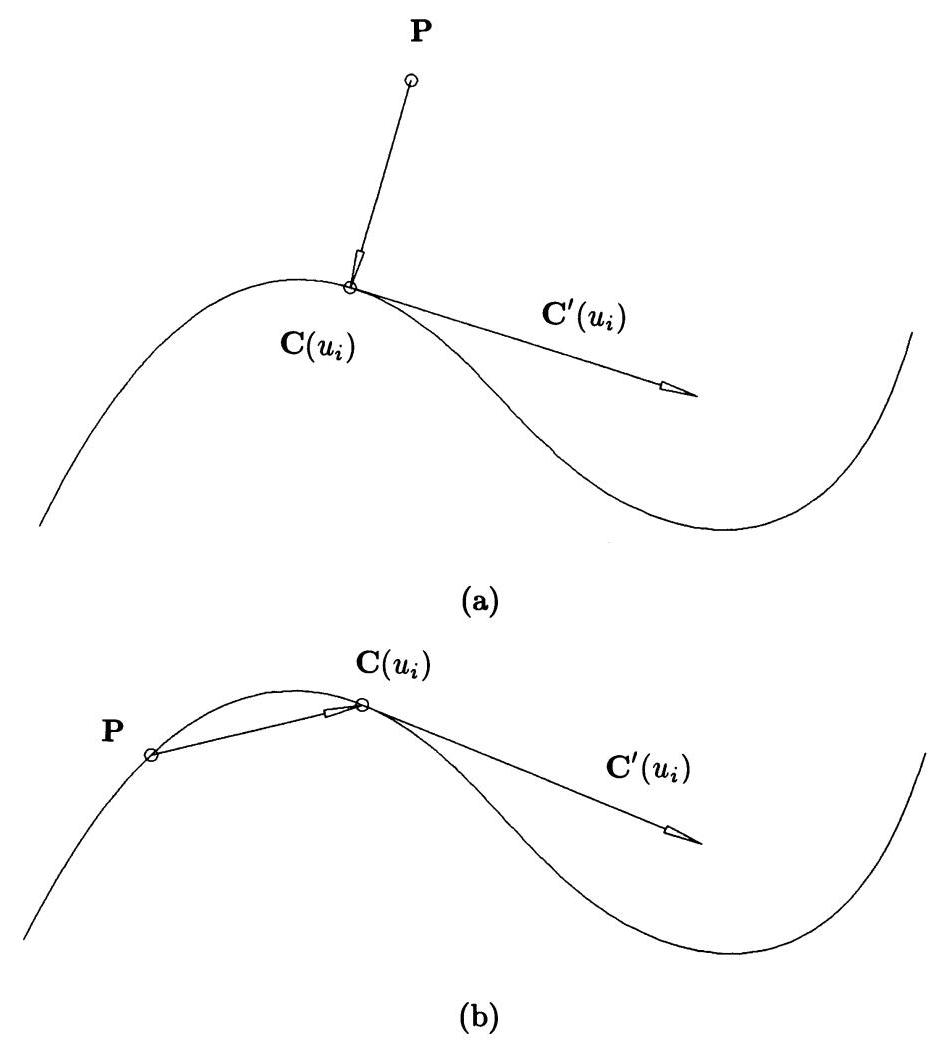
\includegraphics[max width=0.8\textwidth]{images/0193ba0d-ab19-7138-9798-cb281ce60de0_240_297_256_940_1043_0.jpg}
\end{center}
\hspace*{3em} 

图 6.1. (a) 点投影；(b) 点反演。

收敛标准由以下给出

\[
\left| {\left( {{u}_{i + 1} - {u}_{i}}\right) {\mathbf{C}}^{\prime }\left( {u}_{i}\right) }\right|  \leq  {\epsilon }_{1}
\]

\[
\left| {\mathbf{C}\left( {u}_{i}\right)  - \mathbf{P}}\right|  \leq  {\epsilon }_{1}
\]

\[
\frac{\left| {\mathbf{C}}^{\prime }\left( {u}_{i}\right)  \cdot  \left( \mathbf{C}\left( {u}_{i}\right)  - \mathbf{P}\right) \right| }{\left| {{\mathbf{C}}^{\prime }\left( {u}_{i}\right) }\right| \left| {\mathbf{C}\left( {u}_{i}\right)  - \mathbf{P}}\right| } \leq  {\epsilon }_{2} \tag{6.4}
\]

标准按以下顺序检查:

1. 点重合:

\[
\left| {\mathbf{C}\left( {u}_{i}\right)  - \mathbf{P}}\right|  \leq  {\epsilon }_{1}
\]

2. 零余弦:

\[
\frac{\left| {\mathbf{C}}^{\prime }\left( {u}_{i}\right)  \cdot  \left( \mathbf{C}\left( {u}_{i}\right)  - \mathbf{P}\right) \right| }{\left| {{\mathbf{C}}^{\prime }\left( {u}_{i}\right) }\right| \left| {\mathbf{C}\left( {u}_{i}\right)  - \mathbf{P}}\right| } \leq  {\epsilon }_{2}
\]

如果至少有一个条件不满足，则使用公式 (6.3) 计算一个新值 \({u}_{i + 1}\) 。然后检查另外两个条件:

3. 确保参数保持在范围 \(\left( {{u}_{i + 1} \in  \left\lbrack  {a,b}\right\rbrack  }\right)\) 内

如果曲线不是闭合的:

\[
\text{ if }\left( {{u}_{i + 1} < a}\right) \;{u}_{i + 1} = a
\]

\[
\text{ if }\left( {{u}_{i + 1} > b}\right) \;{u}_{i + 1} = b
\]

如果曲线是闭合的:

\[
\text{ if }\left( {{u}_{i + 1} < a}\right) \;{u}_{i + 1} = b - \left( {a - {u}_{i + 1}}\right)
\]

\[
\text{ if }\left( {{u}_{i + 1} > b}\right) \;{u}_{i + 1} = a + \left( {{u}_{i + 1} - b}\right)
\]

4. 参数没有显著变化，例如，点位于曲线的末端之外

\[
\left| {\left( {{u}_{i + 1} - {u}_{i}}\right) {\mathbf{C}}^{\prime }\left( {u}_{i}\right) }\right|  \leq  {\epsilon }_{1}
\]

如果条件 (1)、(2) 或 (4) 中的任何一个满足，则停止迭代。图 6.2 显示了一组点投影到 NURBS 曲线上的情况。

点反演和表面的投影是类似的。形成向量函数

\[
\mathbf{r}\left( {u,v}\right)  = \mathbf{S}\left( {u,v}\right)  - \mathbf{P}
\]

和两个标量方程

\[
f\left( {u,v}\right)  = \mathbf{r}\left( {u,v}\right)  \cdot  {\mathbf{S}}_{u}\left( {u,v}\right)  = 0
\]

\[
g\left( {u,v}\right)  = \mathbf{r}\left( {u,v}\right)  \cdot  {\mathbf{S}}_{v}\left( {u,v}\right)  = 0 \tag{6.5}
\]

\begin{center}
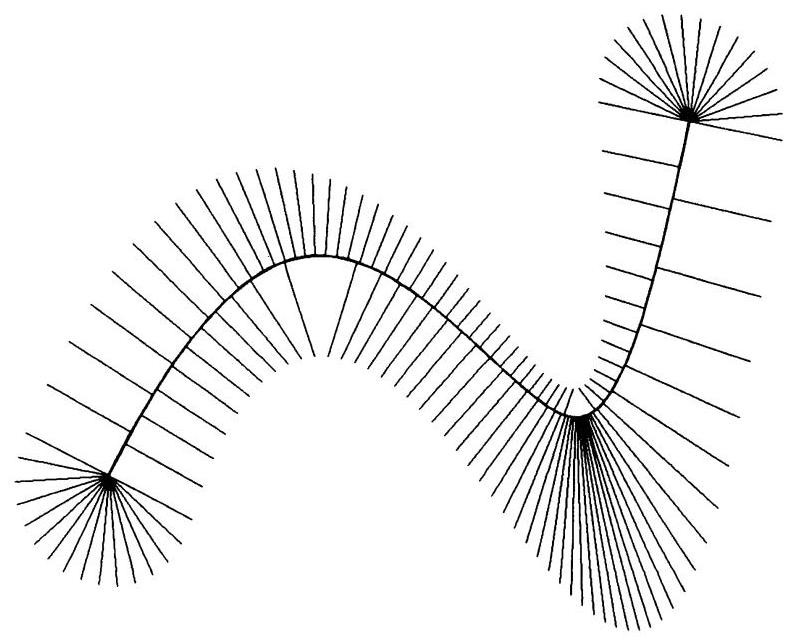
\includegraphics[max width=0.7\textwidth]{images/0193ba0d-ab19-7138-9798-cb281ce60de0_241_369_1443_791_639_0.jpg}
\end{center}
\hspace*{3em} 

图 6.2. 将一组点投影到 NURBS 曲线。

我们必须求解方程 (6.5)。设

\[
{\delta }_{i} = \left\lbrack  \begin{matrix} {\Delta u} \\  {\Delta v} \end{matrix}\right\rbrack   = \left\lbrack  \begin{matrix} {u}_{i + 1} - {u}_{i} \\  {v}_{i + 1} - {v}_{i} \end{matrix}\right\rbrack
\]

\[
{J}_{i} = \left\lbrack  \begin{array}{ll} {f}_{u} & {f}_{v} \\  {g}_{u} & {g}_{v} \end{array}\right\rbrack   = \left\lbrack  \begin{array}{ll} {\left| {\mathbf{S}}_{u}\right| }^{2} + \mathbf{r} \cdot  {\mathbf{S}}_{uu} & {\mathbf{S}}_{u} \cdot  {\mathbf{S}}_{v} + \mathbf{r} \cdot  {\mathbf{S}}_{uv} \\  {\mathbf{S}}_{u} \cdot  {\mathbf{S}}_{v} + \mathbf{r} \cdot  {\mathbf{S}}_{vu} & {\left| {\mathbf{S}}_{v}\right| }^{2} + \mathbf{r} \cdot  {\mathbf{S}}_{vv} \end{array}\right\rbrack
\]

\[
{\kappa }_{i} =  - \left\lbrack  \begin{array}{l} f\left( {{u}_{i},{v}_{i}}\right) \\  g\left( {{u}_{i},{v}_{i}}\right)  \end{array}\right\rbrack
\]

矩阵 \({J}_{i}\) 中的所有函数在 \(\left( {{u}_{i},{v}_{i}}\right)\) 处被评估。在第 \(i\) 次迭代中，我们必须求解未知数 \({\delta }_{i}\) 的 \(2 \times  2\) 线性方程组，给出如下:

\[
{J}_{i}{\delta }_{i} = {\kappa }_{i} \tag{6.6}
\]

从 \({\delta }_{i}\) 我们得到

\[
{u}_{i + 1} = {\Delta u} + {u}_{i}
\]

\[
{v}_{i + 1} = {\Delta v} + {v}_{i} \tag{6.7}
\]

收敛标准由以下给出:

\[
\left| {\left( {{u}_{i + 1} - {u}_{i}}\right) {\mathbf{S}}_{u}\left( {{u}_{i},{v}_{i}}\right)  + \left( {{v}_{i + 1} - {v}_{i}}\right) {\mathbf{S}}_{v}\left( {{u}_{i},{v}_{i}}\right) }\right|  \leq  {\epsilon }_{1}
\]

\[
\left| {\mathbf{S}\left( {{u}_{i},{v}_{i}}\right)  - \mathbf{P}}\right|  \leq  {\epsilon }_{1}
\]

\[
\frac{\left| {\mathbf{S}}_{u}\left( {u}_{i},{v}_{i}\right)  \cdot  \left( \mathbf{S}\left( {u}_{i},{v}_{i}\right)  - \mathbf{P}\right) \right| }{\left| {\mathbf{S}}_{u}\left( {u}_{i},{v}_{i}\right) \right| } \leq  {\epsilon }_{2}\;\frac{\left| {\mathbf{S}}_{v}\left( {u}_{i},{v}_{i}\right)  \cdot  \left( \mathbf{S}\left( {u}_{i},{v}_{i}\right)  - \mathbf{P}\right) \right| }{\left| {{\mathbf{S}}_{v}\left( {{u}_{i},{v}_{i}}\right) }\right| \left| {\mathbf{S}\left( {{u}_{i},{v}_{i}}\right) }\right| \left| {\mathbf{S}\left( {{u}_{i},{v}_{i}}\right)  - \mathbf{P}}\right| } \leq  {\epsilon }_{2}
\]

(6.8)

再次，通过以下方式检查条件:

1. 点重合:

\[
\left| {\mathbf{S}\left( {{u}_{i},{v}_{i}}\right)  - \mathbf{P}}\right|  \leq  {\epsilon }_{1}
\]

2. 零余弦:

\[
\frac{\left| {\mathbf{S}}_{u}\left( {u}_{i},{v}_{i}\right)  \cdot  \left( \mathbf{S}\left( {u}_{i},{v}_{i}\right)  - \mathbf{P}\right) \right| }{\left| {\mathbf{S}}_{u}\left( {u}_{i},{v}_{i}\right) \right| } \leq  {\epsilon }_{2}\;\frac{\left| {\mathbf{S}}_{v}\left( {u}_{i},{v}_{i}\right)  \cdot  \left( \mathbf{S}\left( {u}_{i},{v}_{i}\right)  - \mathbf{P}\right) \right| }{\left| {{\mathbf{S}}_{v}\left( {{u}_{i},{v}_{i}}\right) }\right| \left| {\mathbf{S}\left( {{u}_{i},{v}_{i}}\right) }\right| \left| {\mathbf{S}\left( {{u}_{i},{v}_{i}}\right)  - \mathbf{P}}\right| } \leq  {\epsilon }_{2}
\]

如果这些条件不满足，则使用方程 (6.7) 计算新的值 \(\left( {{u}_{i + 1},{v}_{i + 1}}\right)\) 。然后检查两个条件:

3. 确保参数保持在范围 \(\left( {{u}_{i + 1} \in  \left\lbrack  {a,b}\right\rbrack  }\right.\) 和 \(\left. {{v}_{i + 1} \in  \left\lbrack  {c,d}\right\rbrack  }\right)\) 内:

如果表面在 \(u\) 方向上不闭合:

\[
\text{ if }\left( {{u}_{i + 1} < a}\right) \;{u}_{i + 1} = a
\]

\[
\text{ if }\left( {{u}_{i + 1} > b}\right) \;{u}_{i + 1} = b
\]

如果表面在 \(v\) 方向上不闭合:

\[
\text{ if }\left( {{v}_{i + 1} < c}\right) \;{v}_{i + 1} = c
\]

\[
\text{ if }\left( {{v}_{i + 1} > d}\right) \;{v}_{i + 1} = d
\]

如果表面在 \(u\) 方向上是封闭的:

\[
\text{ if }\left( {{u}_{i + 1} < a}\right) \;{u}_{i + 1} = b - \left( {a - {u}_{i + 1}}\right)
\]

\[
\text{ if }\left( {{u}_{i + 1} > b}\right) \;{u}_{i + 1} = a + \left( {{u}_{i + 1} - b}\right)
\]

如果表面在 \(v\) 方向上是封闭的:

\[
\text{ if }\left( {{v}_{i + 1} < c}\right) \;{v}_{i + 1} = d - \left( {c - {v}_{i + 1}}\right)
\]

\[
\text{ if }\left( {{v}_{i + 1} > d}\right) \;{v}_{i + 1} = c + \left( {{v}_{i + 1} - d}\right)
\]

4. 参数变化不显著，即

\[
\left| {\left( {{u}_{i + 1} - {u}_{i}}\right) {\mathbf{S}}_{u}\left( {{u}_{i},{v}_{i}}\right)  + \left( {{v}_{i + 1} - {v}_{i}}\right) {\mathbf{S}}_{v}\left( {{u}_{i},{v}_{i}}\right) }\right|  \leq  {\epsilon }_{1}
\]

如果满足条件 (1)、(2) 或 (4) 中的任何一个，则停止迭代。图 6.3 显示了控制网的一组点投影到 NURBS 表面上的情况。

\begin{center}
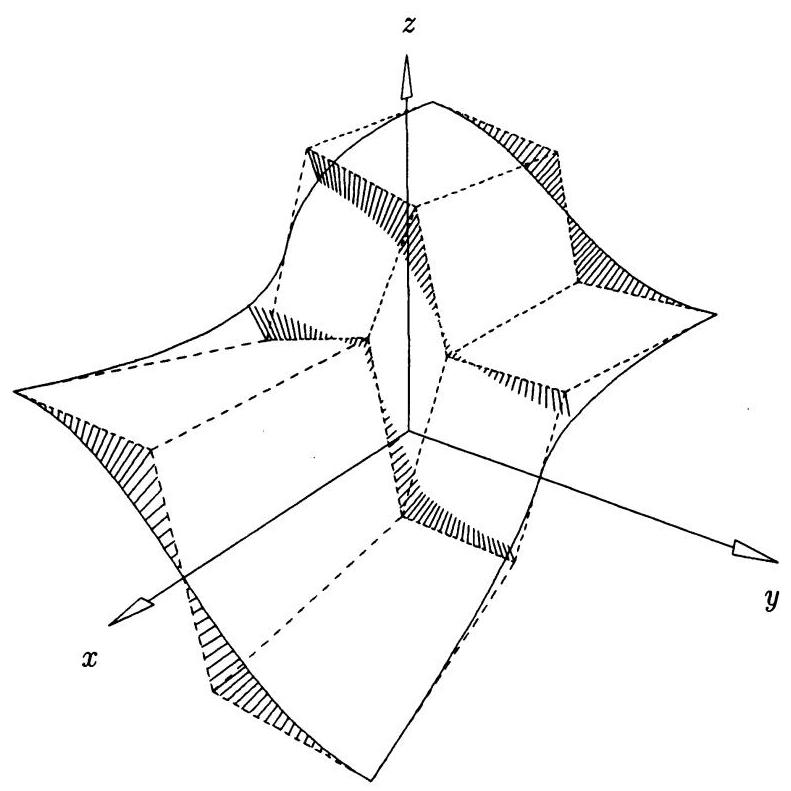
\includegraphics[max width=0.7\textwidth]{images/0193ba0d-ab19-7138-9798-cb281ce60de0_243_372_1269_791_791_0.jpg}
\end{center}
\hspace*{3em} 

图 6.3. 将控制网的点投影到 NURBS 表面上。



\section{曲面切向量反演}

设 \(\left( {\bar{u},\bar{v}}\right)\) 为一个固定参数点， \(\mathbf{P} = \mathbf{S}\left( {\bar{u},\bar{v}}\right)\) 为其在表面 \(\mathbf{S}\left( {u,v}\right)\) 上的像(见图 6.4)。设 \(\mathbf{T} = \left( {{dx},{dy},{dz}}\right)\) 为一个从 \(\mathbf{P}\) 开始并位于 \(\mathbf{S}\left( {u,v}\right)\) 在 \(\mathbf{P}\) 处的切平面上的向量。用 \({\mathbf{S}}_{u}\) 和 \({\mathbf{S}}_{v}\) 表示 \(\mathbf{S}\left( {u,v}\right)\) 在 \(\left( {\bar{u},\bar{v}}\right)\) 处的第一偏导数。如果 \({\mathbf{S}}_{u} \times  {\mathbf{S}}_{v} \neq  0\) ，根据基础微分几何 \(\left\lbrack  {\mathrm{{DoCa}}{76}}\right\rbrack\) ，存在一个向量 \(\mathbf{W} = \left( {{du},{dv}}\right)\) 在 \({uv}\) 平面中，使得

\[
\mathbf{T} = {\mathbf{S}}_{u}{du} + {\mathbf{S}}_{v}{dv} \tag{6.9}
\]

切向量反演是确定向量 \(\mathbf{W}\) 的过程。方程 (6.9) 展开为两个未知数的三个方程，即

\[
\left\lbrack  \begin{array}{ll} {x}_{u} & {x}_{v} \\  {y}_{u} & {y}_{v} \\  {z}_{u} & {z}_{v} \end{array}\right\rbrack  \left\lbrack  \begin{array}{l} {du} \\  {dv} \end{array}\right\rbrack   = \left\lbrack  \begin{array}{l} {dx} \\  {dy} \\  {dz} \end{array}\right\rbrack   \tag{6.10}
\]

我们将其写为

\[
M\mathbf{W} = \mathbf{T}
\]

方程 (6.10) 有一个唯一且精确的解(通常这样的系统没有)，我们通过乘以 \({M}^{T}\) ( \(M\) 的转置)来获得该解。

\[
\left( {{M}^{T}M}\right) \mathbf{W} = {M}^{T}\mathbf{T}
\]

\begin{center}
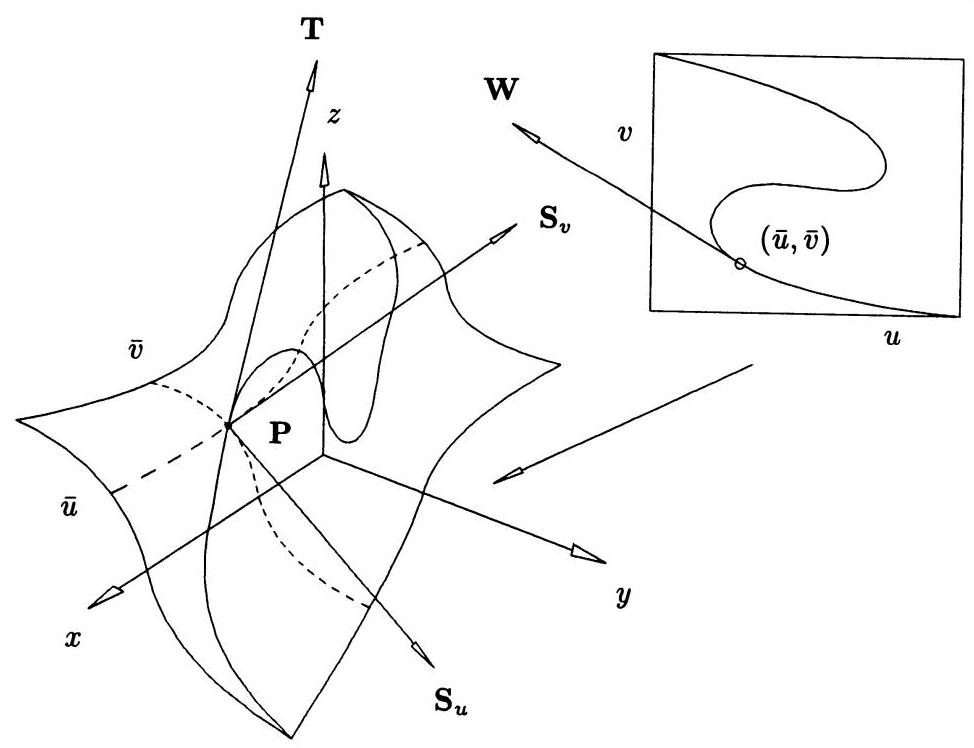
\includegraphics[max width=0.8\textwidth]{images/0193ba0d-ab19-7138-9798-cb281ce60de0_244_284_1310_974_748_0.jpg}
\end{center}
\hspace*{3em} 

图 6.4. 表面切向量反演。

或

\[
\left\lbrack  \begin{array}{ll} {\left| {\mathbf{S}}_{u}\right| }^{2} & {\mathbf{S}}_{u} \cdot  {\mathbf{S}}_{v} \\  {\mathbf{S}}_{u} \cdot  {\mathbf{S}}_{v} & {\left| {\mathbf{S}}_{v}\right| }^{2} \end{array}\right\rbrack  \left\lbrack  \begin{array}{l} {du} \\  {dv} \end{array}\right\rbrack   = \left\lbrack  \begin{array}{l} {\mathbf{S}}_{u} \cdot  \mathbf{T} \\  {\mathbf{S}}_{v} \cdot  \mathbf{T} \end{array}\right\rbrack   \tag{6.11}
\]

解这个 \(2 \times  2\) 方程组可以得到未知数 \({du}\) 和 \({dv}\) 。



\section{曲线和曲面的变换与投影}

曲线和曲面的变换与投影在几何建模和计算机图形学中是常见的。变换包括平移、旋转、缩放、剪切和反射。平行投影和透视投影在视频屏幕或其他二维输出设备上查看三维几何体时是必不可少的。文献中对变换和投影有许多优秀的讨论，例如 [Faux81; Fole90; Roge90]。在本节中，我们假设读者熟悉一般概念，我们仅详细阐述这些概念在 NURBS 曲线和曲面上的应用。

所有变换和投影都是通过对控制点和权重应用操作来对 NURBS 曲线和曲面进行的；因此，讨论可以限制在曲线上。方程 (4.1) 和 (4.5) 表示了思考 NURBS 曲线的两种不同方式，即作为欧几里得空间中的分段有理曲线，或作为齐次空间中的非有理 B 样条曲线。第一种方法使用 B 样条基函数来混合加权的三维控制点；第二种方法使用函数来混合四维控制点。因此，存在两种执行变换和投影的方法:

\begin{itemize}
\item 将操作应用于 \(\mathbf{C}\left( u\right)\) 的三维控制点；对于透视投影，还必须计算新的权重；
\end{itemize}

\begin{itemize}
\item 将 \(4 \times  4\) 矩阵应用于 \({\mathbf{C}}^{w}\left( u\right)\) 的四维控制点。
\end{itemize}

设

\[
\mathbf{C}\left( u\right)  = \frac{\mathop{\sum }\limits_{{i = 0}}^{n}{N}_{i,p}\left( u\right) {w}_{i}{\mathbf{P}}_{i}}{\mathop{\sum }\limits_{{i = 0}}^{n}{N}_{i,p}\left( u\right) {w}_{i}} = \mathop{\sum }\limits_{{i = 0}}^{n}{R}_{i,p}\left( u\right) {\mathbf{P}}_{i} \tag{6.12}
\]

除了透视，所有对 \(\mathbf{C}\left( u\right)\) 的变换和投影都是通过对三维控制点 \({\mathbf{P}}_{i}\) 应用操作来执行的；权重 \({w}_{i}\) 不会改变。这遵循仿射不变性属性 P4.9(该属性源于方程 [6.12] 的形式)。让我们考虑投影。图 6.5 显示了控制点 \({\mathbf{P}}_{i}\) 的一般平行投影到由参考点 \(\mathbf{Q}\) 和单位长度法向量 \(\mathbf{N}.{\overline{\mathbf{P}}}_{i}\) 给定的投影平面上，表示 \({\mathbf{P}}_{i}\) 的投影。如果投影的方向由向量 \(\mathbf{W}\) 给出，那么

\[
{\overline{\mathbf{P}}}_{i} = {\mathbf{P}}_{i} + \alpha \mathbf{W} \tag{6.13}
\]

\begin{center}
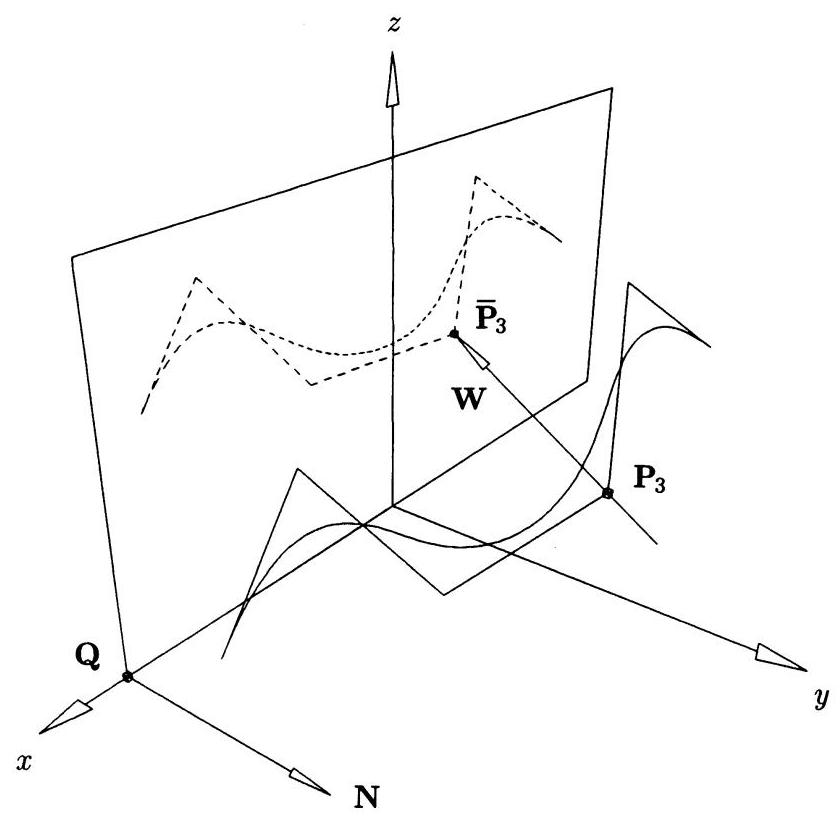
\includegraphics[max width=0.7\textwidth]{images/0193ba0d-ab19-7138-9798-cb281ce60de0_246_348_251_840_819_0.jpg}
\end{center}
\hspace*{3em} 

图 6.5. NURBS 曲线的平行投影。

从方程 (6.13) 我们得到

\[
\alpha \mathbf{W} = {\overline{\mathbf{P}}}_{i} - {\mathbf{P}}_{i} - \mathbf{Q} + \mathbf{Q}
\]

和

\[
\alpha \left( {\mathbf{N} \cdot  \mathbf{W}}\right)  = \mathbf{N} \cdot  \left( {{\overline{\mathbf{P}}}_{i} - \mathbf{Q}}\right)  + \mathbf{N} \cdot  \left( {\mathbf{Q} - {\mathbf{P}}_{i}}\right)
\]

由于 \({\overline{\mathbf{P}}}_{i}\) 位于投影平面 \(\mathbf{N} \cdot  \left( {{\overline{\mathbf{P}}}_{i} - \mathbf{Q}}\right)  = 0\) 上，因此得出

\[
\alpha  = \frac{\mathbf{N} \cdot  \left( {\mathbf{Q} - {\mathbf{P}}_{i}}\right) }{\mathbf{N} \cdot  \mathbf{W}}
\]

最后

\[
{\overline{\mathbf{P}}}_{i} = {\mathbf{P}}_{i} + \left( \frac{\mathbf{N} \cdot  \left( {\mathbf{Q} - {\mathbf{P}}_{i}}\right) }{\mathbf{N} \cdot  \mathbf{W}}\right) \mathbf{W} \tag{6.14}
\]

对于曲面的相应公式是

\[
{\overline{\mathbf{P}}}_{i,j} = {\mathbf{P}}_{i,j} + \left( \frac{\mathbf{N} \cdot  \left( {\mathbf{Q} - {\mathbf{P}}_{i,j}}\right) }{\mathbf{N} \cdot  \mathbf{W}}\right) \mathbf{W} \tag{6.15}
\]

图 6.6 显示了透视投影。与之前一样，设投影平面由 \(\mathbf{Q}\) 和 \(\mathbf{N}\) 定义。将眼睛位置表示为 \(\mathbf{E}\) 。那么

\[
{\overline{\mathbf{P}}}_{i} = \left( {1 - \alpha }\right) {\mathbf{P}}_{i} + \alpha \mathbf{E} \tag{6.16}
\]

\begin{center}
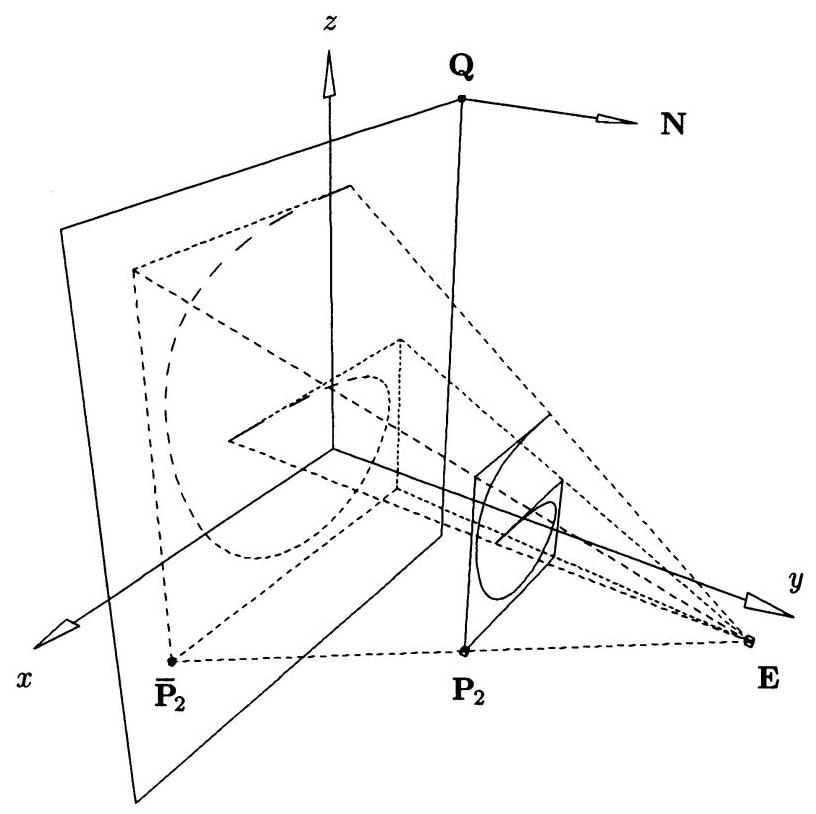
\includegraphics[max width=0.7\textwidth]{images/0193ba0d-ab19-7138-9798-cb281ce60de0_247_362_250_816_814_0.jpg}
\end{center}
\hspace*{3em} 

图 6.6. NURBS 曲线的透视投影。

因此得出

\[
\alpha \left( {\mathbf{E} - {\mathbf{P}}_{i}}\right)  = {\overline{\mathbf{P}}}_{i} - {\mathbf{P}}_{i} - \mathbf{Q} + \mathbf{Q}
\]

而 \(\mathbf{N} \cdot  \left( {{\overline{\mathbf{P}}}_{i} - \mathbf{Q}}\right)  = 0\) 意味着

\[
\alpha  = \frac{\mathbf{N} \cdot  \left( {\mathbf{Q} - {\mathbf{P}}_{i}}\right) }{\mathbf{N} \cdot  \left( {\mathbf{E} - {\mathbf{P}}_{i}}\right) }
\]

从

\[
1 - \alpha  = 1 - \frac{\mathbf{N} \cdot  \left( {\mathbf{Q} - {\mathbf{P}}_{i}}\right) }{\mathbf{N} \cdot  \left( {\mathbf{E} - {\mathbf{P}}_{i}}\right) } = \frac{\mathbf{N} \cdot  \left( {\mathbf{E} - {\mathbf{P}}_{i} - \mathbf{Q} + {\mathbf{P}}_{i}}\right) }{\mathbf{N} \cdot  \left( {\mathbf{E} - {\mathbf{P}}_{i}}\right) } = \frac{\mathbf{N} \cdot  \left( {\mathbf{E} - \mathbf{Q}}\right) }{\mathbf{N} \cdot  \left( {\mathbf{E} - {\mathbf{P}}_{i}}\right) }
\]

我们得到

\[
{\overline{\mathbf{P}}}_{i} = \frac{\mathbf{N} \cdot  \left( {\mathbf{E} - \mathbf{Q}}\right) }{\mathbf{N} \cdot  \left( {\mathbf{E} - {\mathbf{P}}_{i}}\right) }{\mathbf{P}}_{i} + \frac{\mathbf{N} \cdot  \left( {\mathbf{Q} - {\mathbf{P}}_{i}}\right) }{\mathbf{N} \cdot  \left( {\mathbf{E} - {\mathbf{P}}_{i}}\right) }\mathbf{E} \tag{6.17}
\]

方程 (6.17) 是计算投影曲线的新控制点的公式。

现在我们推导新权重的公式。设

\[
\mathbf{P} = \mathbf{C}\left( u\right)  = \mathop{\sum }\limits_{{i = 0}}^{n}{R}_{i,p}\left( u\right) {\mathbf{P}}_{i}
\]

为 \(\mathbf{C}\left( u\right)\) 上的一个任意点，记 \(\overline{\mathbf{P}}\) 为 \(\mathbf{P}\) 的透视投影

到由 \(\mathbf{Q}\) 和 \(\mathbf{N}\) 给出的平面上。回顾一下

\[
\mathop{\sum }\limits_{{i = 0}}^{n}{R}_{i,p}\left( u\right)  = 1
\]

对于所有 \(u\) ，我们得到

\[
\overline{\mathbf{P}} = \frac{\mathbf{N} \cdot  \left( {\mathbf{E} - \mathbf{Q}}\right) }{\mathbf{N} \cdot  \left( {\mathbf{E} - \mathbf{P}}\right) }\mathbf{P} + \frac{\mathbf{N} \cdot  \left( {\mathbf{Q} - \mathbf{P}}\right) }{\mathbf{N} \cdot  \left( {\mathbf{E} - \mathbf{P}}\right) }\mathbf{E}
\]

\[
= \frac{\sum {R}_{i,p}\left( {\mathbf{N} \cdot  \left( {\mathbf{E} - \mathbf{Q}}\right) {\mathbf{P}}_{i}}\right) +\sum {R}_{i,p}\left( {\mathbf{N} \cdot  \left( {\mathbf{Q} - {\mathbf{P}}_{i}}\right) }\right) \mathbf{E}}{\sum {R}_{i,p}\left( {\mathbf{N} \cdot  \left( {\mathbf{E} - {\mathbf{P}}_{i}}\right) }\right) }
\]

\[
= \frac{\sum {R}_{i,p}\left( {\mathbf{N} \cdot  \left( {\mathbf{E} - {\mathbf{P}}_{i}}\right) }\right) \left( \frac{\mathbf{N} \cdot  \left( {\mathbf{E} - \mathbf{Q}}\right) }{\mathbf{N} \cdot  \left( {\mathbf{E} - {\mathbf{P}}_{i}}\right) }\right) {\mathbf{P}}_{i}}{\sum {R}_{i,p}\left( {\mathbf{N} \cdot  \left( {\mathbf{E} - {\mathbf{P}}_{i}}\right) }\right) }
\]

\[
+ \frac{\sum {R}_{i,p}\left( {\mathbf{N} \cdot  \left( {\mathbf{E} - {\mathbf{P}}_{i}}\right) }\right) \left( \frac{\mathbf{N} \cdot  \left( {\mathbf{Q} - {\mathbf{P}}_{i}}\right) }{\mathbf{N} \cdot  \left( {\mathbf{E} - {\mathbf{P}}_{i}}\right) }\right) \mathbf{E}}{\sum {R}_{i,p}\left( {\mathbf{N} \cdot  \left( {\mathbf{E} - {\mathbf{P}}_{i}}\right) }\right) }
\]

设置

\[
{\bar{w}}_{i} = {w}_{i}\left( {\mathbf{N} \cdot  \left( {\mathbf{E} - {\mathbf{P}}_{i}}\right) }\right)  \tag{6.18}
\]

并回顾一下

\[
{R}_{i,p} = \frac{{N}_{i,p}{w}_{i}}{\sum {N}_{i,p}{w}_{i}}
\]

我们得到

\[
\overline{\mathbf{P}} = \frac{\sum {N}_{i,p}{\bar{w}}_{i}\left( {\frac{\mathbf{N} \cdot  \left( {\mathbf{E} - \mathbf{Q}}\right) }{\mathbf{N} \cdot  \left( {\mathbf{E} - {\mathbf{P}}_{i}}\right) }{\mathbf{P}}_{i} + \frac{\mathbf{N} \cdot  \left( {\mathbf{Q} - {\mathbf{P}}_{i}}\right) }{\mathbf{N} \cdot  \left( {\mathbf{E} - {\mathbf{P}}_{i}}\right) }\mathbf{E}}\right) }{\sum {N}_{i,p}{\bar{w}}_{i}}
\]

\[
= \frac{\sum {N}_{i,p}\left( u\right) {\bar{w}}_{i}{\overline{\mathbf{P}}}_{i}}{\sum {N}_{i,p}\left( u\right) {\bar{w}}_{i}} \tag{6.19}
\]

方程 (6.19) 显示由方程 (6.17) 和 (6.18) 给出的控制点和权重是投影曲线的控制点和权重。表面公式为

\[
{\overline{\mathbf{P}}}_{i,j} = \frac{\mathbf{N} \cdot  \left( {\mathbf{E} - \mathbf{Q}}\right) }{\mathbf{N} \cdot  \left( {\mathbf{E} - {\mathbf{P}}_{i,j}}\right) }{\mathbf{P}}_{i,j} + \frac{\mathbf{N} \cdot  \left( {\mathbf{Q} - {\mathbf{P}}_{i,j}}\right) }{\mathbf{N} \cdot  \left( {\mathbf{E} - {\mathbf{P}}_{i,j}}\right) }\mathbf{E} \tag{6.20}
\]

和

\[
{\bar{w}}_{i,j} = {w}_{i,j}\left\lbrack  {\mathbf{N} \cdot  \left( {\mathbf{E} - {\mathbf{P}}_{i,j}}\right) }\right\rbrack   \tag{6.21}
\]

图 6.7 显示了 NURBS 曲面的平行投影。

\begin{center}
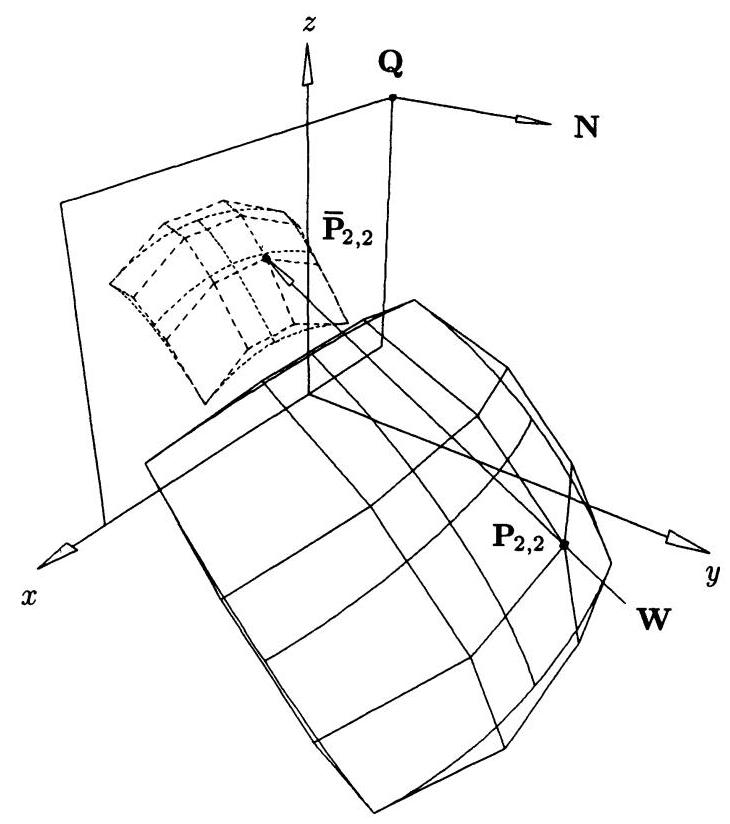
\includegraphics[max width=0.6\textwidth]{images/0193ba0d-ab19-7138-9798-cb281ce60de0_249_403_263_730_824_0.jpg}
\end{center}
\hspace*{3em} 

图 6.7. NURBS 曲面的平行投影。

现在设 \({\mathbf{C}}^{w}\left( u\right)  = \mathop{\sum }\limits_{{i = 0}}^{n}{N}_{i,p}\left( u\right) {\mathbf{P}}_{i}^{w}\) 。所有变换和投影可以被打包成一个 \(4 \times  4\) 形式的矩阵。

\[
A = \left\lbrack  \begin{array}{ll} B & T \\  P & {a}_{3,3} \end{array}\right\rbrack   = \left\lbrack  \begin{array}{llll} {b}_{0,0} & {b}_{0,1} & {b}_{0,2} & {t}_{0} \\  {b}_{1,0} & {b}_{1,1} & {b}_{1,2} & {t}_{1} \\  {b}_{2,0} & {b}_{2,1} & {b}_{2,2} & {t}_{2} \\  {p}_{0} & {p}_{1} & {p}_{2} & {a}_{3,3} \end{array}\right\rbrack   \tag{6.22}
\]

其中向量 \(T\) 和 \(P\) 分别表示平移和透视，而 \(3 \times  3\) 矩阵 \(B\) 包含旋转、缩放、剪切、通过坐标平面的反射以及投影到坐标平面。矩阵 \(A\) 将应用于所有控制点 \({\mathbf{P}}_{i}^{w}\) 的 \({\mathbf{C}}^{w}\left( u\right)\) 。

\section*{示例}

设 \({\mathbf{P}}_{i}^{w} = \left( {{w}_{i}{x}_{i},{w}_{i}{y}_{i},{w}_{i}{z}_{i},{w}_{i}}\right)\) ，并用 \({\overline{\mathbf{P}}}_{i}^{w} = A{\mathbf{P}}_{i}^{w}\) 表示一个变换后的齐次控制点。

Ex6.1 将 \({\mathbf{C}}^{w}\left( u\right)\) 按向量 \(\mathbf{V} = \left( {x,y,z}\right)\) 进行平移。然后

\[
{\overline{\mathbf{P}}}_{i}^{w} = \left\lbrack  \begin{array}{llll} 1 & 0 & 0 & x \\  0 & 1 & 0 & y \\  0 & 0 & 1 & z \\  0 & 0 & 0 & 1 \end{array}\right\rbrack  \left\lbrack  \begin{matrix} {w}_{i}{x}_{i} \\  {w}_{i}{y}_{i} \\  {w}_{i}{z}_{i} \\  {w}_{i} \end{matrix}\right\rbrack   = \left\lbrack  \begin{matrix} {w}_{i}\left( {{x}_{i} + x}\right) \\  {w}_{i}\left( {{y}_{i} + y}\right) \\  {w}_{i}\left( {{z}_{i} + z}\right) \\  {w}_{i} \end{matrix}\right\rbrack
\]

Ex6.2 将旋转矩阵 \(R\) 应用到 \({\mathbf{C}}^{w}\left( u\right)\) 。

\[
{\bar{\mathbf{P}}}_{i}^{w} = \left\lbrack  \begin{matrix} {r}_{0,0} & {r}_{0,1} & {r}_{0,2} & 0 \\  {r}_{1,0} & {r}_{1,1} & {r}_{1,2} & 0 \\  {r}_{2,0} & {r}_{2,1} & {r}_{2,2} & 0 \\  0 & 0 & 0 & 1 \end{matrix}\right\rbrack  \left\lbrack  \begin{matrix} {w}_{i}{x}_{i} \\  {w}_{i}{y}_{i} \\  {w}_{i}{z}_{i} \\  {w}_{i} \end{matrix}\right\rbrack   = \left\lbrack  \begin{matrix} {w}_{i}\left( {{r}_{0,0}{x}_{i} + {r}_{0,1}{y}_{i} + {r}_{0,2}{z}_{i}}\right) \\  {w}_{i}\left( {{r}_{1,0}{x}_{i} + {r}_{1,1}{y}_{i} + {r}_{1,2}{z}_{i}}\right) \\  {w}_{i}\left( {{r}_{2,0}{x}_{i} + {r}_{2,1}{y}_{i} + {r}_{2,2}{z}_{i}}\right) \\  {w}_{i} \end{matrix}\right\rbrack
\]

Ex6.3 透视投影:设 \(\mathbf{E} = \left( {0,0,d}\right)\) 为位于 \(z\) 轴上的眼睛位置，距离原点 \(d\) 。设 \({xy}\) 平面为投影平面。然后

\[
{\overline{\mathbf{P}}}_{i}^{w} = \left\lbrack  \begin{array}{rrrr} d & 0 & 0 & 0 \\  0 & d & 0 & 0 \\  0 & 0 & 0 & 0 \\  0 & 0 &  - 1 & d \end{array}\right\rbrack  \left\lbrack  \begin{matrix} {w}_{i}{x}_{i} \\  {w}_{i}{y}_{i} \\  {w}_{i}{z}_{i} \\  {w}_{i} \end{matrix}\right\rbrack   = \left\lbrack  \begin{matrix} {w}_{i}d{x}_{i} \\  {w}_{i}d{y}_{i} \\  0 \\  {w}_{i}\left( {d - {z}_{i}}\right)  \end{matrix}\right\rbrack   \tag{6.23}
\]


\section{NURBS 曲线和曲面的重参数化}

设 \(\mathbf{C}\left( u\right)  = \left( {x\left( u\right) ,y\left( u\right) ,z\left( u\right) }\right)\) 为 \(u \in  \left\lbrack  {a,b}\right\rbrack\) 上的任意参数曲线，并假设 \(u = f\left( s\right)\) 是在 \(s \in  \left\lbrack  {c,d}\right\rbrack\) 上的标量值函数，满足:

\begin{itemize}
\item 对于所有 \(s \in  \left\lbrack  {c,d}\right\rbrack  \left( {f\left( s\right) \text{ is strictly increasing }}\right)\) 的 \({f}^{\prime }\left( s\right)  > 0\) ;
\end{itemize}

\begin{itemize}
\item \(a = f\left( c\right)\) 和 \(b = f\left( d\right) \left( {f\left( s\right) \text{ maps }\left\lbrack  {c,d}\right\rbrack  \text{ onto }\left\lbrack  {a,b}\right\rbrack  }\right)\) 。
\end{itemize}

\(\mathbf{C}\left( u\right)\) 和 \(f\left( s\right)\) 的组合，由

\[
\mathbf{C}\left( s\right)  = \mathbf{C}\left( {f\left( s\right) }\right)  = \left( {x\left( {f\left( s\right) }\right) ,y\left( {f\left( s\right) }\right) ,z\left( {f\left( s\right) }\right) }\right)
\]

被称为 \(\mathbf{C}\left( u\right)\) 的重新参数化(见图 6.8)。

\(\mathbf{C}\left( s\right)\) 在几何上与 \(\mathbf{C}\left( u\right)\) 是相同的曲线，但在参数上它们是不同的。重新参数化的应用包括:

\begin{itemize}
\item 内部点映射:给定参数值 \({u}_{0},\ldots ,{u}_{n}\) 和 \({s}_{0},\ldots ,{s}_{n}\) ，其中 \(a < {u}_{0} < \cdots  < {u}_{n} < b\) 和 \(c < {s}_{0} < \cdots  < {s}_{n} < d\) ，确定一个函数 \(u = f\left( s\right)\) 使得 \({u}_{i} = f\left( {s}_{i}\right) ,i = 0,\ldots ,n\) 。然后形成 \(\mathbf{C}\left( {f\left( s\right) }\right)\) 。这强制曲线点 \(\mathbf{C}\left( {u}_{i}\right)\) 在新的参数值 \({s}_{i}\) 下被假定；
\end{itemize}

\begin{itemize}
\item 末端导数的修改:重新参数化改变曲线导数；这遵循链式法则，例如。
\end{itemize}

\[
{\mathbf{C}}^{\prime }\left( s\right)  = {\mathbf{C}}^{\prime }\left( u\right) {f}^{\prime }\left( s\right) \;{\mathbf{C}}^{\prime \prime }\left( s\right)  = {\mathbf{C}}^{\prime }\left( u\right) {f}^{\prime \prime }\left( s\right)  + {\mathbf{C}}^{\prime \prime }\left( u\right) {\left( {f}^{\prime }\left( s\right) \right) }^{2}
\]

注意，只有末端一阶导数的大小发生变化，但末端二阶及更高阶导数的大小和方向都会改变；

\begin{itemize}
\item 末端权重的修改:如果 \({\mathbf{C}}^{w}\left( u\right)  = \mathop{\sum }\limits_{{i = 0}}^{n}{N}_{i,p}\left( u\right) {\mathbf{P}}_{i}^{w}\) 是 NURBS
\end{itemize}

\begin{center}
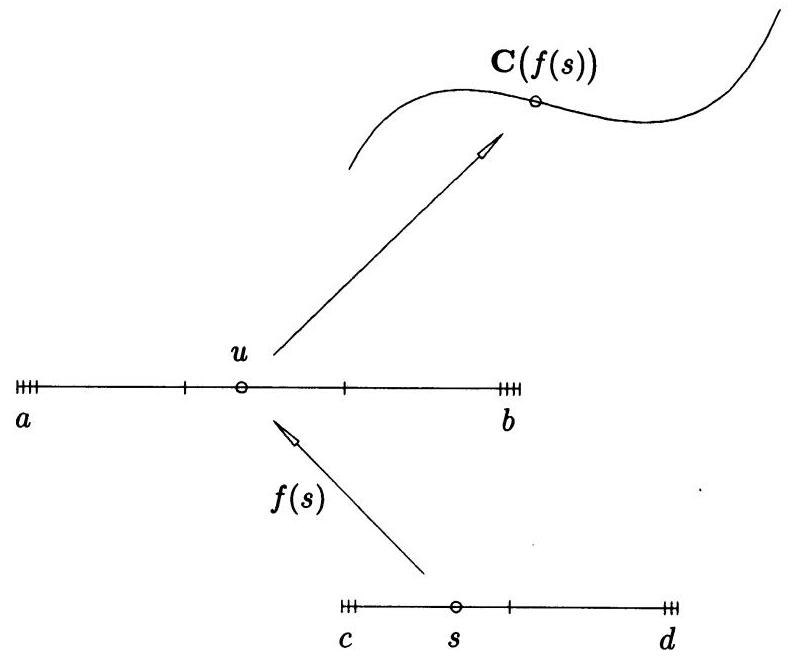
\includegraphics[max width=0.7\textwidth]{images/0193ba0d-ab19-7138-9798-cb281ce60de0_251_372_254_796_663_0.jpg}
\end{center}
\hspace*{3em} 

图 6.8. 曲线重新参数化。

在曲线中，有时修改端点权重 \({w}_{0}\) 和 \({w}_{n}\) 以获得特定值而不改变曲线几何形状是有用的。我们将看到这实际上是可能的，并且简单等同于 \(\mathbf{C}\left( u\right)\) 的重新参数化。

\section*{示例}

Ex6.4 设

\[
\mathbf{C}\left( u\right)  = \left( {x\left( u\right) ,y\left( u\right) }\right)  = \left( {u, - 2{u}^{2} + {2u}}\right)  \tag{6.24}
\]

在 \(u \in  \left\lbrack  {0,1}\right\rbrack\) 上，假设我们希望一个参数 \(s \in  \left\lbrack  {0,1}\right\rbrack\) 使得 \(u = 1/2\) 对应于 \(s = 6/{10}\) ，即

\[
\mathbf{C}\left( {u = \frac{1}{2}}\right)  = \mathbf{C}\left( {s = \frac{6}{10}}\right)  = \left( {\frac{1}{2},\frac{1}{2}}\right)
\]

然后 \(u = f\left( s\right)\) 必须满足三个约束条件

\[
0 = f\left( 0\right) \;\frac{1}{2} = f\left( \frac{6}{10}\right) \;1 = f\left( 1\right)
\]

我们选择 \(f\left( s\right)\) 为二次多项式

\[
u = f\left( s\right)  = a{s}^{2} + {bs} + c
\]

第一个约束意味着 \(c = 0\) ，最后两个产生线性方程

\[
\frac{1}{2} = \frac{9}{25}a + \frac{6}{10}b
\]

\[
1 = a + b \tag{6.25}
\]

解方程 (6.25) 得到

\[
a = \frac{5}{12}\;b = \frac{7}{12}
\]

因此

\[
u = f\left( s\right)  = \frac{5}{12}{s}^{2} + \frac{7}{12}s \tag{6.26}
\]

将方程 (6.26) 代入方程 (6.24)，我们得到重新参数化的曲线

\[
\mathbf{C}\left( s\right)  = \left( {\frac{5}{12}{s}^{2} + \frac{7}{12}s, - \frac{25}{72}{s}^{4} - \frac{35}{36}{s}^{3} + \frac{11}{72}{s}^{2} + \frac{7}{6}s}\right)  \tag{6.27}
\]

读者应验证

\[
\mathbf{C}\left( {s = 0}\right)  = \mathbf{C}\left( {u = 0}\right)  = \left( {0,0}\right)
\]

\[
\mathbf{C}\left( {s = \frac{6}{10}}\right)  = \mathbf{C}\left( {u = \frac{1}{2}}\right)  = \left( {\frac{1}{2}\;,\frac{1}{2}}\right)
\]

\[
\mathbf{C}\left( {s = 1}\right)  = \mathbf{C}\left( {u = 1}\right)  = \left( {0,0}\right)
\]

注意，导数也发生了变化。例如，直接对方程 (6.24) 和 (6.27) 进行求导得到

\[
{\mathbf{C}}^{\prime }\left( {u = 0}\right)  = \left( {1,2}\right) \;{\mathbf{C}}^{\prime }\left( {s = 0}\right)  = \left( {\frac{7}{12},\frac{7}{6}}\right)
\]

图 6.9 显示了曲线及其相对于 \(u\) 和 \(s\) 在 \(u = s = 0\) 处的第一导数。

\begin{center}
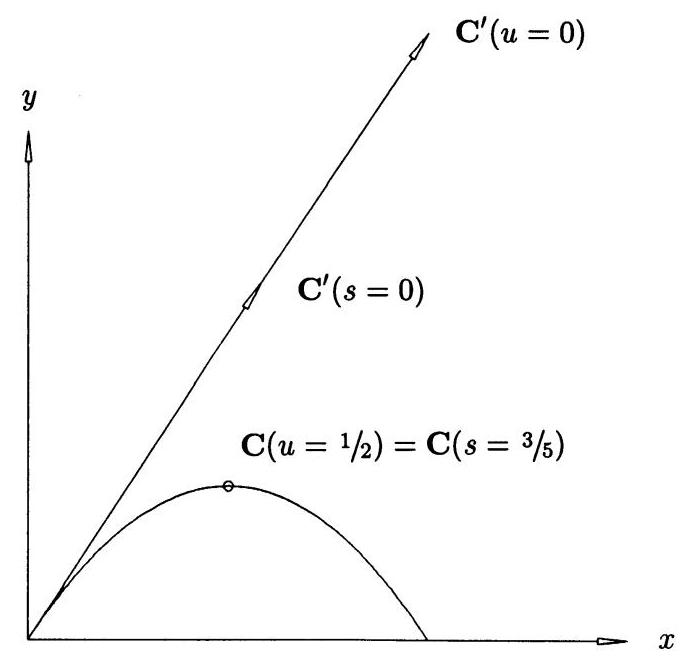
\includegraphics[max width=0.6\textwidth]{images/0193ba0d-ab19-7138-9798-cb281ce60de0_252_420_1421_684_661_0.jpg}
\end{center}
\hspace*{3em} 

图 6.9. 示例 Ex6.4 的重新参数化曲线。

Ex6.5 考虑由以下公式给出的圆弧

\[
\mathbf{C}\left( u\right)  = \left( {\frac{1 - {u}^{2}}{1 + {u}^{2}},\frac{2u}{1 + {u}^{2}}}\right)  \tag{6.28}
\]

在 \(u \in  \left\lbrack  {0,1}\right\rbrack\) 上。该弧以原点为中心，半径为 1，扫过一个角度 \({90}^{ \circ  }\) (见第 1 章，方程 [1.2]，图 1.2，示例 1.8，以及图 1.19a)。很容易检查到

\[
\mathbf{C}\left( {u = \frac{1}{2}}\right)  = \left( {\frac{6}{10},\frac{8}{10}}\right)
\]

和

\[
{\mathbf{C}}^{\prime }\left( {u = 0}\right)  = \left( {0,2}\right)
\]

\[
{\mathbf{C}}^{\prime }\left( {u = 1}\right)  = \left( {-1,0}\right)  \tag{6.29}
\]

我们希望对 \(\mathbf{C}\left( u\right)\) 进行一个更对称的重新参数化 \(\mathbf{C}\left( s\right)\) ，即 \(\mathbf{C}\left( s\right)\) 应满足

\[
\left| {{\mathbf{C}}^{\prime }\left( {s = 0}\right) }\right|  = \left| {{\mathbf{C}}^{\prime }\left( {s = 1}\right) }\right|  \tag{6.30}
\]

我们选择形式为的线性有理函数

\[
u = f\left( s\right)  = \frac{{as} + b}{{cs} + d}\;s \in  \left\lbrack  {0,1}\right\rbrack   \tag{6.31}
\]

显然，我们可以假设 \(d = 1\) ，条件 \(f\left( 0\right)  = 0\) 和 \(f\left( 1\right)  = 1\) 意味着 \(b = 0\) 和 \(c = a - 1\) 。因此， \(f\left( s\right)\) 的形式为

\[
u = \frac{as}{\left( {a - 1}\right) s + 1} \tag{6.32}
\]

方程 (6.30) 给出的条件确定了 \(a\) 。从方程 (6.29) 和 \({\mathbf{C}}^{\prime }\left( s\right)  = {\mathbf{C}}^{\prime }\left( u\right) {f}^{\prime }\left( s\right)\) 中，我们要求

\[
2{f}^{\prime }\left( {s = 0}\right)  = {f}^{\prime }\left( {s = 1}\right)  \tag{6.33}
\]

对方程 (6.32) 求导得到

\[
{f}^{\prime }\left( s\right)  = \frac{a}{{\left( \left( a - 1\right) s + 1\right) }^{2}}
\]

从方程 (6.33) 我们得到 \({2a} = 1/\mathrm{a}\) 。因此 \(2{a}^{2} - 1 = 0\) ，因此 \(a =  \pm  \sqrt{2}/2\) 。选择 \(a =  - \sqrt{2}/2\) 会导致方程 (6.32) 在区间 \(s \in  \left\lbrack  {0,1}\right\rbrack\) 的分母为零，因此我们选择 \(a = \sqrt{2}/2\) 。因此，

我们得到

\[
u = f\left( s\right)  = \frac{\sqrt{2}s}{\left( {\sqrt{2} - 2}\right) s + 2} \tag{6.34}
\]

将方程 (6.34) 代入方程 (6.28) 得到

\[
\mathbf{C}\left( s\right)  = \left( {\frac{\left( {1 - \sqrt{2}}\right) {s}^{2} + \left( {\sqrt{2} - 2}\right) s + 1}{\left( {2 - \sqrt{2}}\right) {s}^{2} + \left( {\sqrt{2} - 2}\right) s + 1},\frac{\left( {1 - \sqrt{2}}\right) {s}^{2} + \sqrt{2}s}{\left( {2 - \sqrt{2}}\right) {s}^{2} + \left( {\sqrt{2} - 2}\right) s + 1}}\right)
\]

(6.35)

读者可以验证 \(\mathbf{C}\left( s\right)\) 满足方程 (6.30) 以及条件

\[
\mathbf{C}\left( {s = \frac{1}{2}}\right)  = \left( {\frac{\sqrt{2}}{2},\frac{\sqrt{2}}{2}}\right)  \tag{6.36}
\]

即 \(s = 1/2\) 映射到圆弧的中点。

\section*{注意:}

\begin{itemize}
\item 如果 \(\mathbf{C}\left( u\right)\) 是一个 \(p\) 次多项式(有理)曲线，而 \(f\left( s\right)\) 是一个 \(q\) 次多项式(有理)函数，则 \(\mathbf{C}\left( s\right)\) 是一个 \({pq}\) 次多项式(有理)曲线。特别地，形式为 \(u = {as} + b\) 或 \(u = \left( {\mathrm{{as}} + \mathrm{b}}\right) /\left( {\mathrm{{cs}} + \mathrm{d}}\right)\) 的线性重新参数化函数不会提高曲线的次数；
\end{itemize}

\begin{itemize}
\item 形式为 \(u = \left( {{as} + b}\right) /\left( {{cs} + d}\right)\) 的线性有理函数将多项式曲线转换为相同次数的有理曲线。
\end{itemize}

现在我们讨论用多项式函数重新参数化 NURBS 曲线的问题。设 \({\mathbf{C}}^{w}\left( u\right)  = \mathop{\sum }\limits_{{i = 0}}^{n}{N}_{i,p}\left( u\right) {\mathbf{P}}_{i}^{w}\) 为 \(p\) 次 NURBS 曲线，定义在 \(u \in  \left\lbrack  {a,b}\right\rbrack\) 上，且 \(u = f\left( s\right)\) 为 \(q\) 次多项式，定义在 \(s \in  \left\lbrack  {c,d}\right\rbrack\) 上。现在假设 \({\mathbf{C}}^{w}\left( u\right)\) 没有内部节点，因此 \(U\) 具有以下形式

\[
U = \{ \underset{p + 1}{\underbrace{a,\ldots ,a}},\underset{p + 1}{\underbrace{b,\ldots ,b}}\}
\]

重新参数化的曲线 \({\mathbf{C}}^{w}\left( s\right)\) 的次数为 \({pq}\) ，并定义在节点向量上

\[
S = \{ \underset{{pq} + 1}{\underbrace{c,\ldots ,c}},\underset{{pq} + 1}{\underbrace{d,\ldots ,d}}\}  \tag{6.37}
\]

新的控制点 \({pq} + 1\) 可以通过链式法则的重复应用和 B 样条曲线的端导数公式计算得出。我们通过示例来说明这一点。

\section*{示例}

Ex6.6 设 \(\mathbf{C}\left( u\right)  = \mathop{\sum }\limits_{{i = 0}}^{2}{N}_{i,2}\left( u\right) {\mathbf{P}}_{i},U = \{ 0,0,0,1,1,1\}\) 为示例 Ex6.4 中抛物弧的 B-spline 表示(见图 6.9 和 6.10)。

控制点为 \(\{ \left( {0,0}\right) ,\left( {1/2,1}\right) ,\left( {1,0}\right) \}\) ，重参数化函数为

\[
u = f\left( s\right)  = \frac{5}{12}{s}^{2} + \frac{7}{12}s\;\text{ on }\;s \in  \left\lbrack  {0,1}\right\rbrack
\]

重参数化的曲线，四次度数，表示为

\[
\mathbf{C}\left( s\right)  = \mathop{\sum }\limits_{{i = 0}}^{4}{N}_{i,4}\left( s\right) {\mathbf{Q}}_{i}\;S = \{ 0,0,0,0,0,1,1,1,1,1\}  \tag{6.38}
\]

显然(见图 6.10)

\[
{\mathbf{Q}}_{0} = {\mathbf{P}}_{0}\;{\mathbf{Q}}_{4} = {\mathbf{P}}_{2}
\]

从 \({\mathbf{C}}^{\prime }\left( s\right)  = {\mathbf{C}}^{\prime }\left( u\right) {f}^{\prime }\left( s\right)\) 和方程 (3.7) 我们得到

\[
{\mathbf{C}}^{\prime }\left( {s = 0}\right)  = \frac{4}{1 - 0}\left( {{\mathbf{Q}}_{1} - {\mathbf{Q}}_{0}}\right)  = {\mathbf{C}}^{\prime }\left( {u = 0}\right) {f}^{\prime }\left( {s = 0}\right)
\]

\[
= \frac{2}{1 - 0}\left( {{\mathbf{P}}_{1} - {\mathbf{P}}_{0}}\right) \left( \frac{7}{12}\right)
\]

\begin{center}
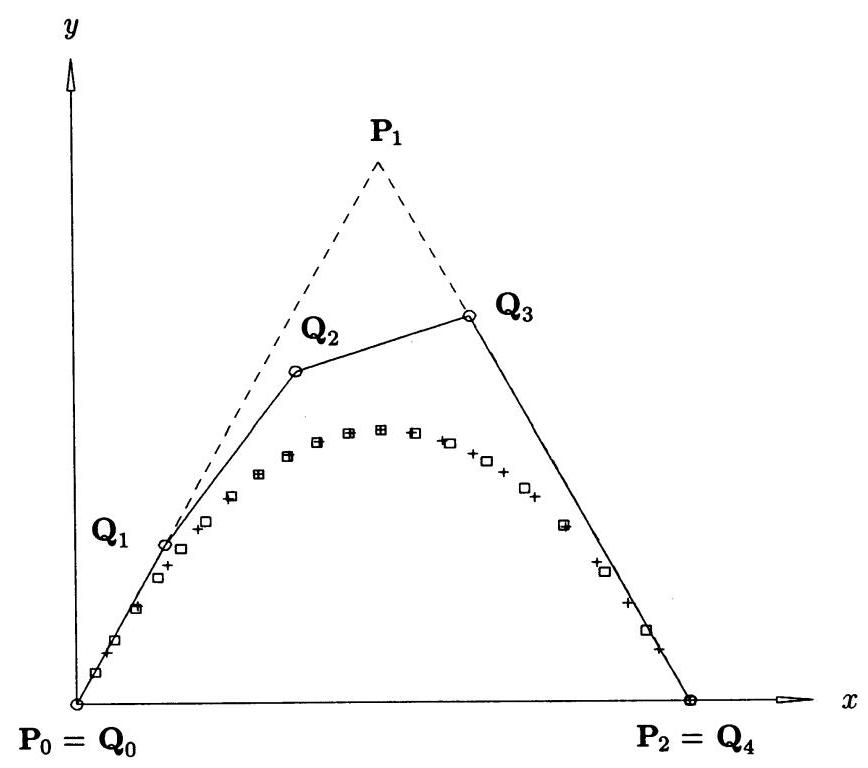
\includegraphics[max width=0.7\textwidth]{images/0193ba0d-ab19-7138-9798-cb281ce60de0_255_334_1280_868_768_0.jpg}
\end{center}
\hspace*{3em} 

图 6.10. 示例 Ex6.6 的重参数化 B-spline 曲线；+ 显示了原始参数化，而 \(\square\) 则说明了新的参数化。

从中得出

\[
{\mathbf{Q}}_{1} = \frac{7}{24}\left( {{\mathbf{P}}_{1} - {\mathbf{P}}_{0}}\right)  + {\mathbf{Q}}_{0} = \left( {\frac{7}{48},\frac{7}{24}}\right)
\]

类似地， \(4\left( {{\mathbf{Q}}_{4} - {\mathbf{Q}}_{3}}\right)  = 2\left( {{\mathbf{P}}_{2} - {\mathbf{P}}_{1}}\right) \left( {{17}/{12}}\right)\) ，和

\[
{\mathbf{Q}}_{3} = {\mathbf{Q}}_{4} - \frac{17}{24}\left( {{\mathbf{P}}_{2} - {\mathbf{P}}_{1}}\right)  = \left( {\frac{31}{48},\frac{17}{24}}\right)
\]

从 \({\mathbf{C}}^{\prime \prime }\left( s\right)  = {\mathbf{C}}^{\prime }\left( u\right) {f}^{\prime \prime }\left( s\right)  + {\mathbf{C}}^{\prime \prime }\left( u\right) {\left( {f}^{\prime }\left( s\right) \right) }^{2}\) 和方程 (3.9) 得出，并注意到

\[
{\mathbf{C}}^{\prime }\left( {u = 0}\right)  = \left( {1,2}\right) \;{\mathbf{C}}^{\prime \prime }\left( {u = 0}\right)  = \left( {0, - 4}\right)
\]

\[
{f}^{\prime }\left( {s = 0}\right)  = \frac{7}{12}\;{f}^{\prime \prime }\left( {s = 0}\right)  = \frac{5}{6}
\]

我们得到

\[
{\mathbf{C}}^{\prime \prime }\left( {s = 0}\right)  = {12}\left( {{\mathbf{Q}}_{0} - 2{\mathbf{Q}}_{1} + {\mathbf{Q}}_{2}}\right)  = \frac{5}{6}\left( {1,2}\right)  + {\left( \frac{7}{12}\right) }^{2}\left( {0, - 4}\right)
\]

从中得出

\[
{\mathbf{Q}}_{2} = \frac{5}{72}\left( {1,2}\right)  + \frac{49}{1728}\left( {0, - 4}\right)  + 2\left( {\frac{7}{48},\frac{7}{24}}\right)  = \left( {\frac{156}{432},\frac{263}{432}}\right)
\]

因此，重新参数化一个没有内部节点的 \(p\) 阶曲线 \({\mathbf{C}}^{w}\left( u\right)\) 为一个 \(q\) 阶多项式 \(f\left( s\right)\) 的一般过程是:

1. 设置 \({\mathbf{Q}}_{0} = {\mathbf{P}}_{0}\) 和 \({\mathbf{Q}}_{pq} = {\mathbf{P}}_{p}\) ；

2. 令 \({\mathbf{C}}^{w\left( i\right) }\) 表示 \({\mathbf{C}}^{w}\left( u\right)\) 的 \(i\) 阶导数，并令 \({m}_{\ell } = \left( {\mathrm{{pq}} + 1}\right) /2\) (整数运算)和 \({m}_{r} = {pq} - \mathrm{{pq}}/2 - 1\) 。计算 \({\mathbf{C}}^{w\left( i\right) }\left( {u = a}\right)\) 的导数 \(i = 1,\ldots ,{m}_{\ell }\) ，以及 \({\mathbf{C}}^{w\left( i\right) }\left( {u = b}\right)\) 的导数 \(i = 1,\ldots ,{m}_{r}\) ；注意，微分是在齐次空间中进行的；

3. 令 \({f}^{\left( i\right) }\) 表示 \(f\left( s\right)\) 的 \(i\) 阶导数；计算 \({f}^{\left( i\right) }(s =\) 的导数 c) 和 \(i = 1,\ldots ,{m}_{\ell }\) 的导数 \({f}^{\left( i\right) }\left( {s = d}\right)\) ，以及 \(i = 1,\ldots ,{m}_{r}\) 的导数；

4. 使用链式法则的重复应用(该法则将 \({\mathbf{C}}^{w\left( i\right) }\left( s\right)\) 表示为 \({\mathbf{C}}^{w\left( i\right) }\left( u\right)\) 和 \(\left. {{f}^{\left( i\right) }\left( s\right) }\right)\) 的函数，并结合方程 (6.41) 和 (6.42)，计算新的控制点 \({\mathbf{Q}}_{1},\ldots ,{\mathbf{Q}}_{{m}_{\ell }}\) 和 \({\mathbf{Q}}_{{pq} - 1},\ldots ,{\mathbf{Q}}_{{pq} - {m}_{r}}\) 。

应用链式法则四次得到

\[
{\mathbf{C}}^{w\left( 1\right) }\left( s\right)  = {\mathbf{C}}^{w\left( 1\right) }\left( u\right) {f}^{\left( 1\right) }\left( s\right)
\]

\[
{\mathbf{C}}^{w\left( 2\right) }\left( s\right)  = {\mathbf{C}}^{w\left( 1\right) }\left( u\right) {f}^{\left( 2\right) }\left( s\right)  + {\mathbf{C}}^{w\left( 2\right) }\left( u\right) {\left( {f}^{\left( 1\right) }\left( s\right) \right) }^{2}
\]

\[
{\mathbf{C}}^{w\left( 3\right) }\left( s\right)  = {\mathbf{C}}^{w\left( 1\right) }\left( u\right) {f}^{\left( 3\right) }\left( s\right)  + 3{\mathbf{C}}^{w\left( 2\right) }\left( u\right) {f}^{\left( 1\right) }\left( s\right) {f}^{\left( 2\right) }\left( s\right)  + {\mathbf{C}}^{w\left( 3\right) }\left( u\right) {\left( {f}^{\left( 1\right) }\left( s\right) \right) }^{3}
\]

248 高级几何算法

\[
{\mathbf{C}}^{w\left( 4\right) }\left( s\right)  = {\mathbf{C}}^{w\left( 1\right) }\left( u\right) {f}^{\left( 4\right) }\left( s\right)  + {\mathbf{C}}^{w\left( 2\right) }\left( u\right) \left\lbrack  {4{f}^{\left( 1\right) }\left( s\right) {f}^{\left( 3\right) }\left( s\right)  + 3{\left( {f}^{\left( 2\right) }\left( s\right) \right) }^{2}}\right\rbrack
\]

\[
+ 6{\mathbf{C}}^{w\left( 3\right) }\left( u\right) {\left( {f}^{\left( 1\right) }\left( s\right) \right) }^{2}{f}^{\left( 2\right) }\left( s\right)  + {\mathbf{C}}^{w\left( 4\right) }\left( u\right) {\left( {f}^{\left( 1\right) }\left( s\right) \right) }^{4} \tag{6.39}
\]

一般公式

\[
{\mathbf{C}}^{w\left( n\right) }\left( s\right)  = \mathop{\sum }\limits_{{j = 0}}^{n}\mathop{\sum }\limits_{\substack{{{k}_{1} + {k}_{2} + \cdots  + {k}_{n} = j} \\  {{k}_{1} + 2{k}_{2} + \cdots  + {k}_{n} = j} \\  {{k}_{1} + 2{k}_{2} + \cdots  + {k}_{n} \geq  0} }}\frac{n!}{{k}_{1}!{\left( 1!\right) }^{{k}_{1}}\cdots {k}_{n}!{\left( n!\right) }^{{k}_{n}}}{\left( {f}^{\left( 1\right) }\left( s\right) \right) }^{{k}_{1}}\cdots {\left( {f}^{\left( n\right) }\left( s\right) \right) }^{{k}_{n}} \tag{6.40}
\]

是由 Faa di Bruno 提出的(见 [Knut73]，第 50 页)。尽管这个公式优雅，但它的实现并不简单。困难在于获得满足条件的 \(n\) -元组

\[
{k}_{1} + {k}_{2} + \cdots  + {k}_{n} = j
\]

\[
{k}_{1} + 2{k}_{2} + \cdots  + n{k}_{n} = n\;{k}_{1},{k}_{2},\ldots ,{k}_{n} \geq  0
\]

为了说明这一点，我们使用方程 (6.40) 推导出方程 (6.39) 中给出的前四个导数:

n=1: \({k}_{1} = 1\) 必须成立:

\[
j = 0 : {k}_{1} = 0 \rightarrow  \text{ no solution }
\]

\[
j = 1 : {k}_{1} = 1 \rightarrow  \left( 1\right)
\]

这导致

\[
{\mathbf{C}}^{w\left( 1\right) }\left( s\right)  = {\mathbf{C}}^{w\left( 1\right) }\left( u\right) {f}^{\left( 1\right) }\left( s\right)
\]

\(\mathrm{n} = 2 : {k}_{1} + 2{k}_{2} = 2\) 必须成立:

\[
j = 0 : {k}_{1} + {k}_{2} = 0 \rightarrow  \text{ no solution }
\]

\[
j = 1 : {k}_{1} + {k}_{2} = 1 \rightarrow  \left( {0,1}\right)
\]

\[
j = 2 : {k}_{1} + {k}_{2} = 2 \rightarrow  \left( {2,0}\right)
\]

产生 \({\mathbf{C}}^{w\left( 2\right) }\left( s\right)  = {\mathbf{C}}^{w\left( 1\right) }\left( u\right) {f}^{\left( 2\right) }\left( s\right)  + {\mathbf{C}}^{w\left( 2\right) }\left( u\right) {\left( {f}^{\left( 1\right) }\left( s\right) \right) }^{2}\)

\(\mathrm{n} = 3 : {k}_{1} + 2{k}_{2} + 3{k}_{3} = 3\) 必须成立:

\[
j = 0 : {k}_{1} + {k}_{2} + {k}_{3} = 0 \rightarrow  \text{ no solution }
\]

\[
j = 1 : {k}_{1} + {k}_{2} + {k}_{3} = 1 \rightarrow  \left( {0,0,1}\right)
\]

\[
j = 2 : {k}_{1} + {k}_{2} + {k}_{3} = 2 \rightarrow  \left( {1,1,0}\right)
\]

\[
j = 3 : {k}_{1} + {k}_{2} + {k}_{3} = 3 \rightarrow  \left( {3,0,0}\right)
\]

从中我们得到

\[
{\mathbf{C}}^{w\left( 3\right) }\left( s\right)  = {\mathbf{C}}^{w\left( 1\right) }\left( u\right) {f}^{\left( 3\right) }\left( s\right)  + 3{\mathbf{C}}^{w\left( 2\right) }\left( u\right) {f}^{\left( 1\right) }\left( s\right) {f}^{\left( 2\right) }\left( s\right)  + {\mathbf{C}}^{w\left( 3\right) }\left( u\right) {\left( {f}^{\left( 1\right) }\left( s\right) \right) }^{3}
\]

\[
\mathrm{n} = 4 : {k}_{1} + 2{k}_{2} + 3{k}_{3} + 4{k}_{4} = 4\text{ must hold: }
\]

\[
j = 0 : {k}_{1} + {k}_{2} + {k}_{3} + {k}_{4} = 0 \rightarrow  \text{ no solution }
\]

\[
j = 1 : {k}_{1} + {k}_{2} + {k}_{3} + {k}_{4} = 1 \rightarrow  \left( {0,0,0,1}\right)
\]

\[
j = 2 : {k}_{1} + {k}_{2} + {k}_{3} + {k}_{4} = 2 \rightarrow  \left( {1,0,1,0}\right) \text{ and }\left( {0,2,0,0}\right)
\]

\[
j = 3 : {k}_{1} + {k}_{2} + {k}_{3} + {k}_{4} = 3 \rightarrow  \left( {2,1,0,0}\right)
\]

\[
j = 4 : {k}_{1} + {k}_{2} + {k}_{3} + {k}_{4} = 4 \rightarrow  \left( {4,0,0,0}\right)
\]

从中我们得到

\[
{\mathbf{C}}^{w\left( 4\right) }\left( s\right)  = {\mathbf{C}}^{w\left( 1\right) }\left( u\right) {f}^{\left( 4\right) }\left( s\right)  + {\mathbf{C}}^{w\left( 2\right) }\left( u\right) \left\lbrack  {4{f}^{\left( 1\right) }\left( s\right) {f}^{\left( 3\right) }\left( s\right)  + 3{\left( {f}^{\left( 2\right) }\left( s\right) \right) }^{2}}\right\rbrack
\]

\[
+ 6{\mathbf{C}}^{w\left( 3\right) }\left( u\right) {\left( {f}^{\left( 1\right) }\left( s\right) \right) }^{2}{f}^{\left( 2\right) }\left( s\right)  + {\mathbf{C}}^{w\left( 4\right) }\left( u\right) {\left( {f}^{\left( 1\right) }\left( s\right) \right) }^{4}
\]

考虑到 \({\mathbf{C}}^{w}\left( s\right)\) 关于 \({\mathbf{C}}^{w}\left( u\right)\) 和 \(f\left( s\right)\) 的导数， \({\mathbf{Q}}_{i}^{w}\) 的一般公式为

\[
{\mathbf{Q}}_{i}^{w} = \frac{\left( {{pq} - i}\right) !\Delta {s}^{i}}{\left( {pq}\right) !}{\mathbf{C}}^{w\left( i\right) }\left( {s = c}\right)  + \mathop{\sum }\limits_{{j = 0}}^{{i - 1}}{\left( -1\right) }^{i + j - 1}\left( \begin{array}{l} i \\  j \end{array}\right) {\mathbf{Q}}_{j}^{w} \tag{6.41}
\]

其中 \(\Delta {s}^{i} = {\left( d - c\right) }^{i},i = 1,\ldots ,{m}_{\ell }\) ，和

\[
{\mathbf{Q}}_{{pq} - i}^{w} = {\left( -1\right) }^{i}\frac{\left( {{pq} - i}\right) !\Delta {s}^{i}}{\left( {pq}\right) !}{\mathbf{C}}^{w\left( i\right) }\left( {s = d}\right)  + \mathop{\sum }\limits_{{j = 0}}^{{i - 1}}{\left( -1\right) }^{i + j - 1}\left( \begin{array}{l} i \\  j \end{array}\right) {\mathbf{Q}}_{{pq} - j}^{w} \tag{6.42}
\]

对于 \(i = 1,\ldots ,{m}_{r}\) 。例如，左侧的前五个控制点是

\[
{\mathbf{Q}}_{0}^{w} = {\mathbf{P}}_{0}^{w}
\]

\[
{\mathbf{Q}}_{1}^{w} = \frac{\Delta s}{pq}{\mathbf{C}}^{w\left( 1\right) }\left( {s = c}\right)  + {\mathbf{Q}}_{0}^{w}
\]

\[
{\mathbf{Q}}_{2}^{w} = \frac{\Delta {s}^{2}}{{pq}\left( {{pq} - 1}\right) }{\mathbf{C}}^{w\left( 2\right) }\left( {s = c}\right)  - {\mathbf{Q}}_{0}^{w} + 2{\mathbf{Q}}_{1}^{w}
\]

\[
{\mathbf{Q}}_{3}^{w} = \frac{\Delta {s}^{3}}{{pq}\left( {{pq} - 1}\right) \left( {{pq} - 2}\right) }{\mathbf{C}}^{w\left( 3\right) }\left( {s = c}\right)  + {\mathbf{Q}}_{0}^{w} - 3{\mathbf{Q}}_{1}^{w} + 3{\mathbf{Q}}_{2}^{w}
\]

\[
{\mathbf{Q}}_{4}^{w} = \frac{\Delta {s}^{4}}{{pq}\left( {{pq} - 1}\right) \left( {{pq} - 2}\right) \left( {{pq} - 3}\right) }{\mathbf{C}}^{w\left( 4\right) }\left( {s = c}\right)  - {\mathbf{Q}}_{0}^{w} + 4{\mathbf{Q}}_{1}^{w} - 6{\mathbf{Q}}_{2}^{w} + 4{\mathbf{Q}}_{3}^{w}
\]

(6.43)

右侧的控制点是

\[
{\mathbf{Q}}_{pq}^{w} = {\mathbf{P}}_{n}^{w}
\]

\[
{\mathbf{Q}}_{{pq} - 1}^{w} =  - \frac{\Delta s}{pq}{\mathbf{C}}^{w\left( 1\right) }\left( {s = d}\right)  + {\mathbf{Q}}_{pq}^{w}
\]

\[
{\mathbf{Q}}_{{pq} - 2}^{w} = \frac{\Delta {s}^{2}}{{pq}\left( {{pq} - 1}\right) }{\mathbf{C}}^{w\left( 2\right) }\left( {s = d}\right)  - {\mathbf{Q}}_{pq}^{w} + 2{\mathbf{Q}}_{{pq} - 1}^{w}
\]

\[
{\mathbf{Q}}_{{pq} - 3}^{w} =  - \frac{\Delta {s}^{3}}{{pq}\left( {{pq} - 1}\right) \left( {{pq} - 2}\right) }{\mathbf{C}}^{w\left( 3\right) }\left( {s = d}\right)  + {\mathbf{Q}}_{pq}^{w} - 3{\mathbf{Q}}_{{pq} - 1}^{w} + 3{\mathbf{Q}}_{{pq} - 2}^{w}
\]

\[
{\mathbf{Q}}_{{pq} - 4}^{w} = \frac{\Delta {s}^{4}}{{pq}\left( {{pq} - 1}\right) \left( {{pq} - 2}\right) \left( {{pq} - 3}\right) }{\mathbf{C}}^{w\left( 4\right) }\left( {s = d}\right)  - {\mathbf{Q}}_{pq}^{w}
\]

\[
+ 4{\mathbf{Q}}_{{pq} - 1}^{w} - 6{\mathbf{Q}}_{{pq} - 2}^{w} + 4{\mathbf{Q}}_{{pq} - 3}^{w} \tag{6.44}
\]

线性重新参数化函数

\[
u = {\alpha s} + \beta \;s \in  \left\lbrack  {c,d}\right\rbrack   \tag{6.45}
\]

是一个有趣的特例。检查方程 (6.39)，注意到

\[
{\mathbf{C}}^{w\left( i\right) }\left( s\right)  = {\mathbf{C}}^{w\left( i\right) }\left( u\right) {\left( {f}^{\left( 1\right) }\left( s\right) \right) }^{i} = {\alpha }^{i}{\mathbf{C}}^{w\left( i\right) }\left( u\right)  \tag{6.46}
\]

然后

\[
{\mathbf{Q}}_{1}^{w} = \frac{\Delta s}{pq}{\mathbf{C}}^{w\left( 1\right) }\left( s\right)  + {\mathbf{Q}}_{0}^{w} = \frac{\alpha \Delta s}{\Delta u}\left( {{\mathbf{P}}_{1}^{w} - {\mathbf{P}}_{0}^{w}}\right)  + {\mathbf{P}}_{0}^{w} \tag{6.47}
\]

从 \(a = {\alpha c} + \beta\) 和 \(b = {\alpha d} + \beta\) 我们得到

\[
\alpha  = \frac{b - a}{d - c} = \frac{\Delta u}{\Delta s} \tag{6.48}
\]

将方程 (6.48) 代入方程 (6.47) 得到

\[
{\mathbf{Q}}_{1}^{w} = {\mathbf{P}}_{1}^{w}
\]

使用方程 (6.41)、(6.46) 和 (6.48)，可以通过归纳法证明

\[
{\mathbf{Q}}_{i}^{w} = {\mathbf{P}}_{i}^{w}\;\text{ for all }i \tag{6.49}
\]

因此，既不改变次数也不改变(齐次)控制点；方程 (6.45) 的线性函数仅仅将参数范围从 \(\left\lbrack  {a,b}\right\rbrack\) 改变为 \(\left\lbrack  {c,d}\right\rbrack\) 。

现在让 \({\mathbf{C}}^{w}\left( u\right)\) 是在 \(u \in  \left\lbrack  {a,b}\right\rbrack\) 上的任意 \(p\) 次 NURBS 曲线，其节点向量为 \(U\) ，并且让 \(u = f\left( s\right)\) 是在 \(s \in  \left\lbrack  {c,d}\right\rbrack\) 上的 \(q\) 次分段多项式重新参数化函数。现在 \(f\left( s\right)\) 可以是任何形式，但为了方便术语，我们假设它是 B 样条形式，即

\[
u = f\left( s\right)  = \mathop{\sum }\limits_{{i = 0}}^{n}{N}_{i,q}\left( s\right) {f}_{i} \tag{6.50}
\]

其中 \(\left\{  {f}_{i}\right\}\) 是标量。用 \(S\) 表示节点向量；那么 \({\mathbf{C}}^{w}\left( {f\left( s\right) }\right)\) 是在 \(s \in  \left\lbrack  {c,d}\right\rbrack\) 上的 \({pq}\) 次 NURBS 曲线，其节点和控制点可以如下计算:

1. 设 \(\left\{  {s}_{i}\right\}\) 表示 \(f\left( s\right)\) 的一组不同的内部节点，设 \(\left\{  {u}_{i}\right\}   =\)  \(\left\{  {f\left( {s}_{i}\right) }\right\}\) 表示它们的映像；使用节点细化插入所有 \({u}_{i}\) 和 \(U\) 的所有原始内部节点，直到它们都具有重数 \(p.{\mathbf{C}}^{w}\left( u\right)\) ，然后在分段 Bézier 形式中；用 \({U}^{\prime }\) 表示细化后的节点向量；

2. 设

\[
s = g\left( u\right)  = {f}^{-1}\left( s\right)  \tag{6.51}
\]

是 \(f\left( s\right)\) 的反函数；然后形成新的节点向量 \({S}^{\prime }\) ，其不同的节点是 \({s}_{i} = g\left( {u}_{i}\right)\) 的不同节点的像 \({U}^{\prime }\) 。所有内部节点在 \({S}^{\prime }\) 中出现的重数为 \({pq}\) ；

3. 使用方程 (6.39)-(6.44) 和在步骤 2 中从新的 \(s\) 节点获得的 \(\Delta {s}_{i}\) 来计算 \({\mathbf{C}}^{w}\left( s\right)\) 的新控制点，该控制点也以分段贝塞尔形式表示；

4. 对 \({\mathbf{C}}^{w}\left( s\right)\) 和 \({S}^{\prime }\) 应用节点移除，以获得 \({\mathbf{C}}^{w}\left( s\right)\) 的最小表示。已知 \({\mathbf{C}}^{w}\left( s\right)\) 的连续性及其节点的重数，因此不需要一般的节点移除(如算法 A5.5 中所示)。设 \({s}_{i}\) 为 \({S}^{\prime }\) 中的一个节点，设 \({u}_{i} = f\left( {s}_{i}\right)\) ；用 \({m}_{i}^{u}\) 和 \({m}_{i}^{s}\) 表示原始节点向量 \(U\) 和 \(S\) 中 \({u}_{i}\) 和 \({s}_{i}\) 的重数，分别为 \(\left( {{m}_{i}^{u},{m}_{i}^{s} \geq  0}\right)\) 。那么 \({s}_{i}\) 在 \({S}^{\prime }\) 中的重数 \({m}_{i}\) 为

\[
{m}_{i} = {pq} - p + {m}_{i}^{u}\;\text{ if }{m}_{i}^{s} = 0
\]

\[
{m}_{i} = {pq} - q + {m}_{i}^{s}\;\text{ if }{m}_{i}^{u} = 0
\]

\[
{m}_{i} = \max \left( {{pq} - p + {m}_{i}^{u},{pq} - q + {m}_{i}^{s}}\right) \;\text{ if }{m}_{i}^{u} \neq  0,{m}_{i}^{s} \neq  0 \tag{6.52}
\]

如果 \(u = f\left( s\right)  = {\alpha s} + \beta\) ，那么 \(s = g\left( u\right)  = \left( {u - \beta }\right) /\alpha\) 。(齐次) 控制点不变，新节点是通过从原始节点获得的

\[
{s}_{i} = g\left( {u}_{i}\right)  \tag{6.53}
\]

例如，节点向量 \(U = \{ 0,0,0,1/3,1,1,1\}\) 和 \({S}^{\prime } = \{ 1,1,1,3,7,7,7\}\) 是等价的(定义相同的曲线)，因为 \(s = {6u} + 1\) 将 \(U\) 映射到 \({S}^{\prime }\) 。

图 6.11a-6.11d 显示了重新参数化的示例。曲线是定义在 \(U = \{ 0,0,0,0,1/2,1,1,1,1\}\) 上的三次 B 样条曲线。在图 6.11a 中，重新参数化函数(显示在右上角)由标量 \(F = \{ 0,2{/}_{5},1\}\) 定义，位于节点向量 \(S = \{ 0,0,0,1,1,1\}\) 上。图 6.11b 显示了由 \(F = \left\{  {0,2/5,9/{10},1}\right\}\) 和 \(S = \{ 0,0,0,1/2,1,1,1\}\) 定义的重新参数化。在图 6.11c 中，该函数由 \(F = \{ 0,1/2,7/{10},9/{10},1\}\) 和 \(S = \{ 0,0,0\) 、 \(\left. {1/2,1/2,1,1,1}\right\}\) 给出。图 6.11d 描绘了使用线性 B 样条函数进行的重新参数化，该函数由 \(F = \{ 0,1\}\) 和 \(S = \{ 0,0,1,1\}\) 给出。

现在我们转向使用有理(或分段有理)函数进行重新参数化。

形式为

\[
u = f\left( s\right)  = \frac{g\left( s\right) }{h\left( s\right) } \tag{6.54}
\]

(a) \(F = \{ 0,2/5,1\} ,S = \{ 0,0,0,1,1,1\}\) ; (b) \(F = \{ 0,2/5,9/{10},1\} ,S = \{ 0,0,0,1/2,1,1,1\}\) 。

\begin{center}
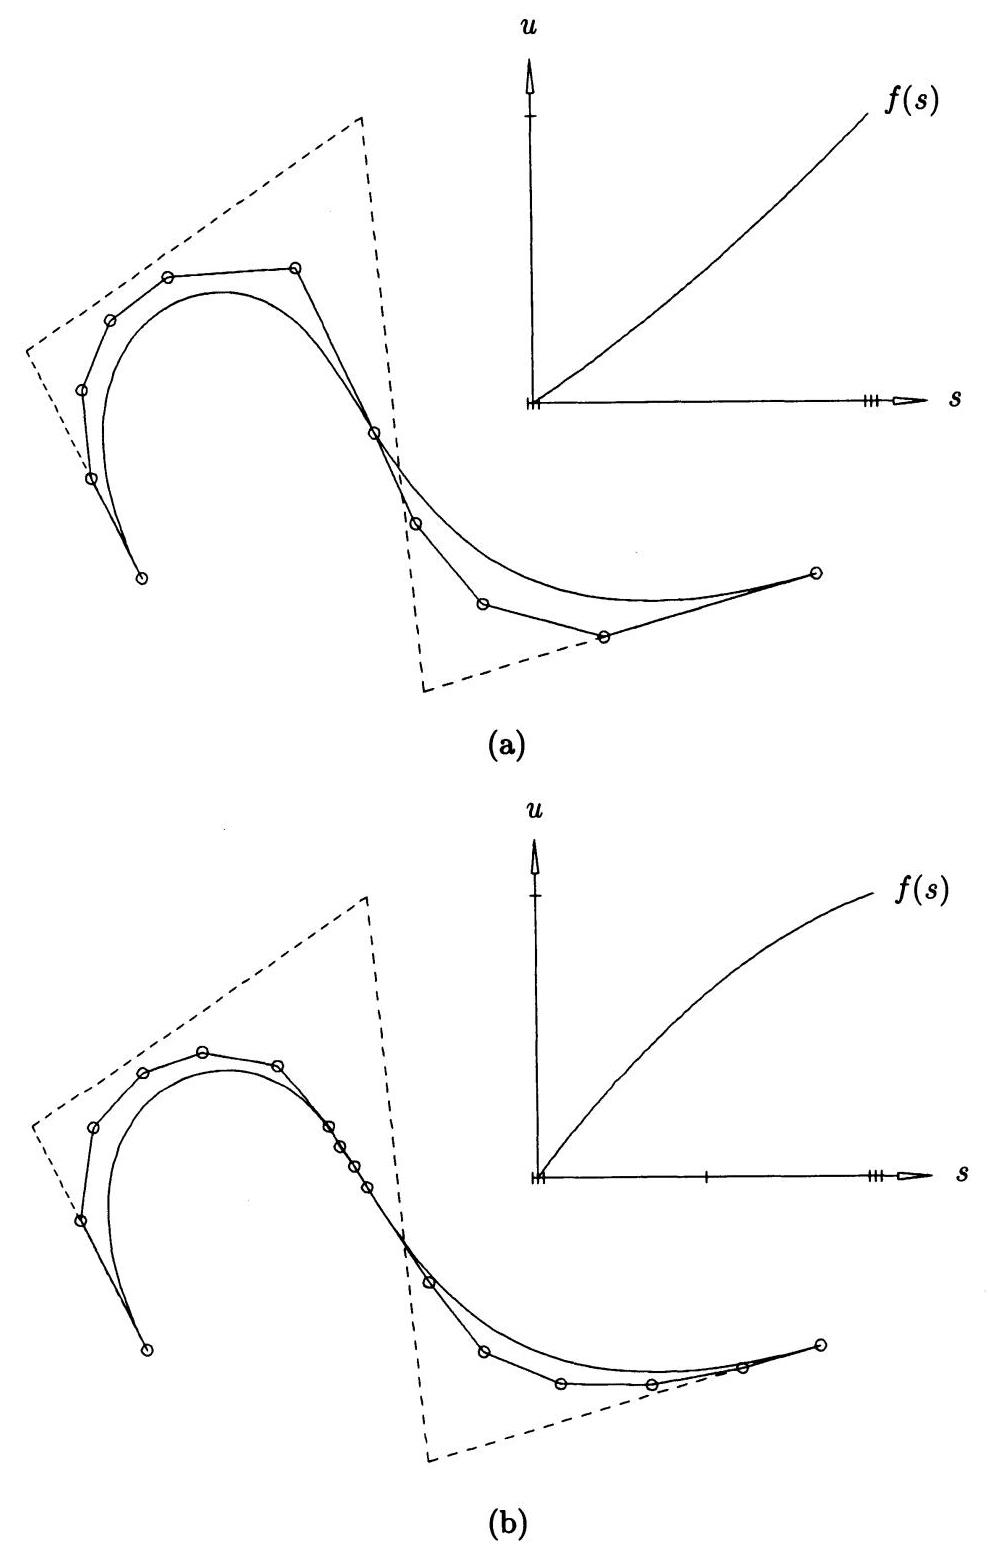
\includegraphics[max width=0.9\textwidth]{images/0193ba0d-ab19-7138-9798-cb281ce60de0_261_268_250_990_1547_0.jpg}
\end{center}
\hspace*{3em} 

图 6.11. 使用二次 B 样条函数重新参数化的 B 样条曲线。

如前所述，如果 \({\mathbf{C}}^{w}\left( u\right)\) 或 \(f\left( s\right)\) 有内部节点，我们可以分三步进行重新参数化:

1. 插入节点以获得 \({\mathbf{C}}^{w}\left( u\right)\) 作为分段贝塞尔曲线；

2. 重新参数化贝塞尔段；

3. 移除不必要的节点。

\begin{center}
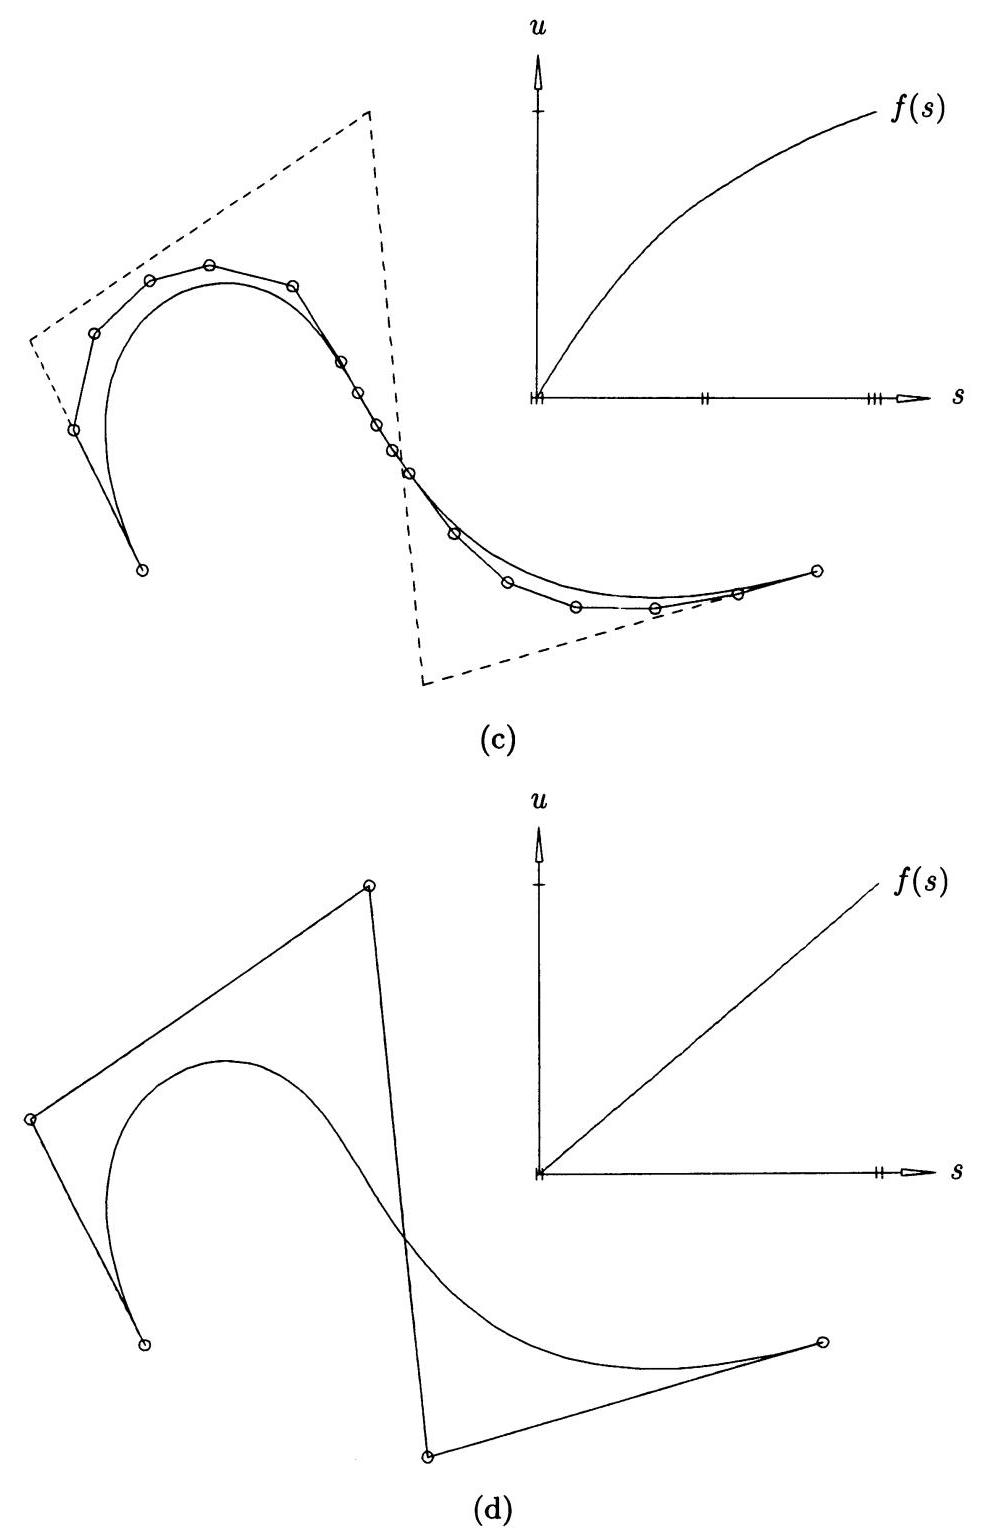
\includegraphics[max width=0.9\textwidth]{images/0193ba0d-ab19-7138-9798-cb281ce60de0_262_277_248_988_1537_0.jpg}
\end{center}
\hspace*{3em} 

图 6.11. (续)(c) \(F = \left\{  {0,1/2,7/{10},9/{10},1}\right\}  ,S = \{ 0,0,0,1/2,1/2,1,1,1\}\) ; (d) \(F = \{ 0,1\} ,S = \{ 0,0,1,1\}\) 。

因此，我们可以假设 \({\mathbf{C}}^{w}\left( u\right)\) 和 \(f\left( s\right)\) 没有内部节点。从理论上讲，可以使用类似于多项式函数的技术通过有理函数进行重新参数化。设 \(r\left( u\right)  = \mathop{\sum }\limits_{{i = 0}}^{p}{a}_{i}{u}^{i}\) 为一个 \(p\) 次多项式。

函数。那么

\[
r\left( s\right)  = r\left( \frac{g\left( s\right) }{h\left( s\right) }\right)  = \mathop{\sum }\limits_{{i = 0}}^{p}{a}_{i}{\left( \frac{g\left( s\right) }{h\left( s\right) }\right) }^{i}
\]

254 高级几何算法

和

\[
\bar{r}\left( s\right)  = {\left( h\left( s\right) \right) }^{p}r\left( s\right)  = \mathop{\sum }\limits_{{i = 0}}^{p}{a}_{i}{\left( g\left( s\right) \right) }^{i}{\left( h\left( s\right) \right) }^{p - i}
\]

如果 \(g\left( s\right)\) 和 \(h\left( s\right)\) 是 \(q\) 次多项式，那么 \(\bar{r}\left( s\right)\) 是一个 \({pq}\) 次多项式。现在设

\[
{\mathbf{C}}^{w}\left( u\right)  = \left( {{wx}\left( u\right) ,{wy}\left( u\right) ,{wz}\left( u\right) ,w\left( u\right) }\right)
\]

为一个 \(p\) 次多项式曲线在齐次空间中。那么

\[
{\mathbf{C}}^{w}\left( s\right)  = {\mathbf{C}}^{w}\left( \frac{g\left( s\right) }{h\left( s\right) }\right)  = \left\lbrack  {{wx}\left( \frac{g\left( s\right) }{h\left( s\right) }\right) ,\ldots ,w\left( \frac{g\left( s\right) }{h\left( s\right) }\right) }\right\rbrack
\]

和

\[
{\overline{\mathbf{C}}}^{w}\left( s\right)  = {\left( h\left( s\right) \right) }^{p}{\mathbf{C}}^{w}\left( s\right)  = \left\lbrack  {{\left( h\left( s\right) \right) }^{p}{wx}\left( \frac{g\left( s\right) }{h\left( s\right) }\right) ,\ldots ,{\left( h\left( s\right) \right) }^{p}w\left( \frac{g\left( s\right) }{h\left( s\right) }\right) }\right\rbrack
\]

关于 \({\overline{\mathbf{C}}}^{w}\left( s\right)\) ，注意到

\begin{itemize}
\item \({\overline{\mathbf{C}}}^{w}\left( s\right)\) 是一个 \({pq}\) 次多项式曲线在齐次空间中；
\end{itemize}

\begin{itemize}
\item \({\overline{\mathbf{C}}}^{w}\left( s\right)\) 和 \({\mathbf{C}}^{w}\left( s\right)\) 是齐次空间中的不同曲线，但它们在欧几里得空间中投影为同一曲线，即 \(\overline{\mathbf{C}}\left( s\right)  = \mathbf{C}\left( s\right)\) ；
\end{itemize}

\begin{itemize}
\item 使用 \({\overline{\mathbf{C}}}^{w}\left( s\right)  = {\left( h\left( s\right) \right) }^{p}{\mathbf{C}}^{w}\left( {\mathrm{\;g}\left( \mathrm{\;s}\right) /\mathrm{h}\left( \mathrm{s}\right) }\right)\) 、链式法则和末端导数公式，可以计算 \({\overline{\mathbf{C}}}^{w}\left( s\right)\) 的新齐次控制点。
\end{itemize}

使用有理函数与多项式函数进行重新参数化的根本区别是:

\begin{itemize}
\item 如果 \(f\left( s\right)\) 是多项式，则 \({\mathbf{C}}^{w}\left( u\right)\) (因此 \(\mathbf{C}\left( u\right)\) )被重新参数化，但 \({\mathbf{C}}^{w}\left( u\right)\) 在几何上没有改变；此外， \(\mathbf{C}\left( u\right)\) 的末端权重不变；
\end{itemize}

\begin{itemize}
\item 如果 \(f\left( s\right)\) 是有理的，则生成不同的曲线 \({\overline{\mathbf{C}}}^{w}\left( s\right)\) ，它投影到相同的(但重新参数化的)曲线 \(\mathbf{C}\left( u\right)\) 。一般来说， \(\mathbf{C}\left( u\right)\) 的末端权重会改变。
\end{itemize}

\section*{示例}

Ex6.7 由方程 (6.35) 给出的圆弧具有贝塞尔表示。显然，欧几里得控制点 \(\left\{  {\mathbf{P}}_{i}\right\}   = \{ \left( {1,0}\right) ,\left( {1,1}\right) ,\left( {0,1}\right) \}\) 保持不变。权重通过将方程 (6.35) 的分母函数的幂基和贝塞尔形式相等来确定。

\[
\left( {2 - \sqrt{2}}\right) {s}^{2} + \left( {\sqrt{2} - 2}\right) s + 1 = {\left( 1 - s\right) }^{2}{w}_{0} + {2s}\left( {1 - s}\right) {w}_{1} + {s}^{2}{w}_{2}
\]

代入 \(s = 0,1,1/2\) ，并求解 \({w}_{i}\) 得到

\[
\left\{  {w}_{i}\right\}   = \left\{  {1,\frac{\sqrt{2}}{2},1}\right\}   \tag{6.55}
\]

图 6.12 显示了新曲线 \({\overline{\mathbf{C}}}^{w}\left( s\right)\) 及其投影 \(\mathbf{C}\left( s\right)\) 。将此图与图 1.22 进行比较。

在实践中，通常不需要使用高于一阶的有理重新参数化函数。Lee 和 Lucian [Lee91] 对使用线性有理函数的重新参数化进行了出色的描述。我们在此总结他们的结果。设

\[
\mathbf{C}\left( u\right)  = \frac{\mathop{\sum }\limits_{{i = 0}}^{n}{N}_{i,p}\left( u\right) {w}_{i}{\mathbf{P}}_{i}}{\mathop{\sum }\limits_{{i = 0}}^{n}{N}_{i,p}\left( u\right) {w}_{i}}\;u \in  \left\lbrack  {a,b}\right\rbrack
\]

\[
s = g\left( u\right)  = \frac{{\alpha u} + \beta }{{\gamma u} + \delta }
\]

\[
u = f\left( s\right)  = \frac{-{\delta s} + \beta }{{\gamma s} - \alpha }\;s \in  \left\lbrack  {c,d}\right\rbrack
\]

\(\left( {f\left( s\right) \text{ is the inverse of }g\left( u\right) }\right)\) 。设

\[
\mu \left( u\right)  = {\gamma u} + \delta \;\lambda \left( s\right)  = {\gamma s} - \alpha
\]

为确保 \(g\left( u\right)\) 和 \(f\left( s\right)\) 表现良好，我们假设

\[
{\alpha \delta } - {\gamma \beta } > 0
\]

\(\mu \left( u\right)  \neq  0\;\) 对所有 \(u \in  \left\lbrack  {a,b}\right\rbrack\)

\(\lambda \left( s\right)  \neq  0\) 对所有 \(s \in  \left\lbrack  {c,d}\right\rbrack\) 重新参数化的曲线 \(\mathbf{C}\left( s\right)\) 如下获得:

\begin{center}
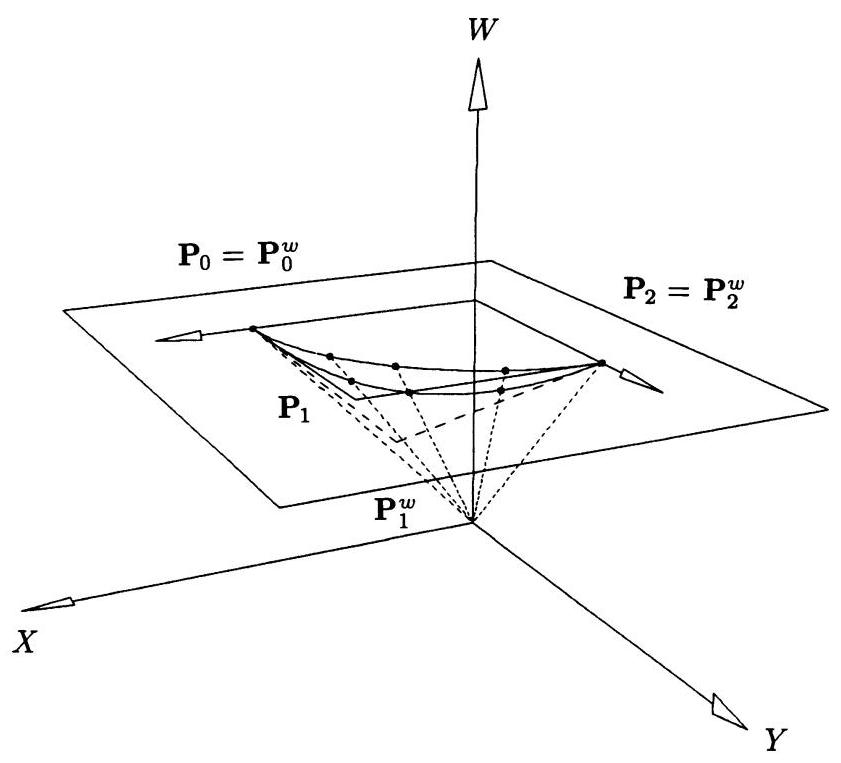
\includegraphics[max width=0.7\textwidth]{images/0193ba0d-ab19-7138-9798-cb281ce60de0_264_347_1327_841_763_0.jpg}
\end{center}
\hspace*{3em} 

图 6.12. 使用权重 \(\left\{  {1,\sqrt{2}/2,1}\right\}\) 的圆弧的均匀表示。

1. 控制点 \(\left\{  {\mathbf{P}}_{i}\right\}\) 不变；

2. 新的节点是原始节点在 \(g\left( u\right)\) 下的映像， \({s}_{i} = g\left( {u}_{i}\right)\) ；

3. 新的权重 \(\left\{  {\bar{w}}_{i}\right\}\) (模一个共同的非零因子)是通过

通过

\[
{\bar{w}}_{i} = {w}_{i}\mathop{\prod }\limits_{{j = 1}}^{p}\lambda \left( {s}_{i + j}\right)  \tag{6.56}
\]

或

\[
{\bar{w}}_{i} = \frac{{w}_{i}}{\mathop{\prod }\limits_{{j = 1}}^{p}\mu \left( {u}_{i + j}\right) } \tag{6.57}
\]

\({s}_{i + j}\) 和 \({u}_{i + j}\) 分别是新的和旧的节点。

图 6.13a 到 \({6.13}\mathrm{c}\) 显示了重新参数化的例子。三次 NURBS 曲线最初在节点向量 \(U = \{ 0,0,0,0,{}^{3}{/}_{10},\)  \(7/{10},1,1,1,1\}\) 上定义。在图 \({6.13}\mathrm{a}\) 和 \({6.13}\mathrm{\;b}\) 中，所有权重最初都等于一。在图 \({6.13}\mathrm{c}\) 中，原始权重为 \(W = \{ 1,1/2,2,3,1/2,1\}\) 。在图 6.13a 中，合理函数是

\[
g\left( u\right)  = \frac{{2u} + 1}{{3u} + 2}
\]

\begin{center}
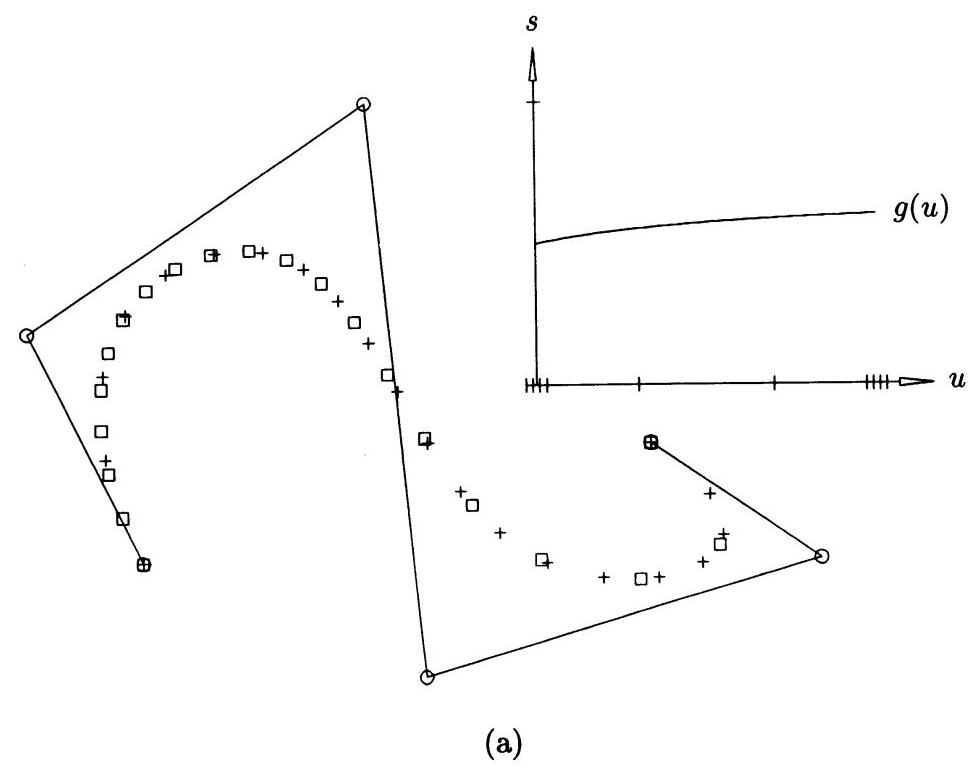
\includegraphics[max width=0.9\textwidth]{images/0193ba0d-ab19-7138-9798-cb281ce60de0_265_271_1252_979_768_0.jpg}
\end{center}
\hspace*{3em} 

图 6.13. NURBS 曲线的合理重新参数化；+ 显示了原始参数化，而 \(\square\) 说明了新的参数化。(a) \(g\left( u\right)  = \left( {{2u} + 1}\right) /\left( {{3u} + 2}\right)\) ；(b) \(g\left( u\right)  = {}^{2u}/{}_{\left( 3u + 1\right) }\) ；(c) \(g\left( u\right)  = {}^{\left( 2u - 1\right) }/{}_{\left( 3u + 2\right) }\) 。

图 6.13.(续)。

\begin{center}
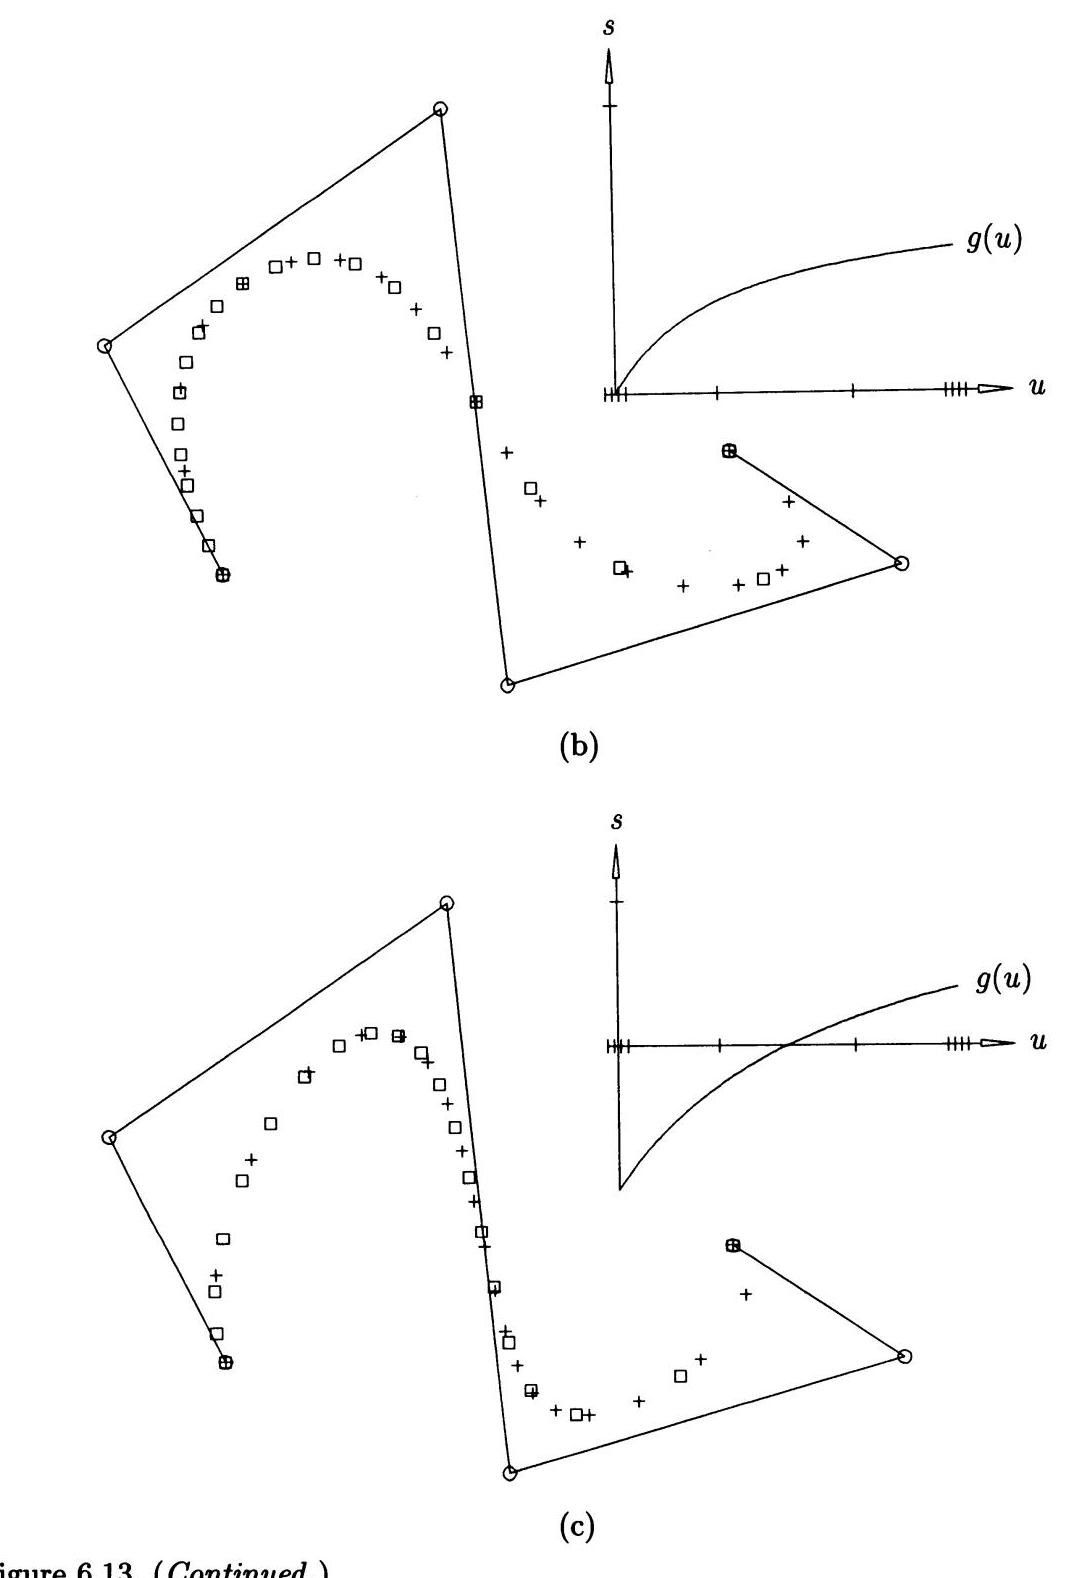
\includegraphics[max width=0.9\textwidth]{images/0193ba0d-ab19-7138-9798-cb281ce60de0_266_196_250_1069_1578_0.jpg}
\end{center}
\hspace*{3em} 

导致新的节点向量

\[
U = \{ {0.5},{0.5},{0.5},{0.5},{0.55},{0.58},{0.6},{0.6},{0.6},{0.6}\}
\]

和权重

\[
W = \{ {0.125},{0.08},{0.04},{0.01},{0.009},{0.008}\}
\]

+ 显示了原始参数化，而 \(\square\) 标记了新的参数化。图 6.13b

应用

\[
g\left( u\right)  = \frac{2u}{{3u} + 1}
\]

产生

\[
U = \{ 0,0,0,0,{0.31},{0.45},{0.5},{0.5},{0.5},{0.5}\}
\]

和

\[
W = \{ {1.0},{0.52},{0.16},{0.04},{0.02},{0.01}\}
\]

再次，+ 显示了原始参数化，而 \(\square\) 显示了新的参数化。最后，在

图 6.13c 中，该函数

\[
g\left( u\right)  = \frac{{2u} - 1}{{3u} + 2}
\]

产生 \(\;U = \{  - {0.5}, - {0.5}, - {0.5}, - {0.5}, - {0.13},{0.09},{0.2},{0.2},{0.2},{0.2}\}\)

和

\[
W = \{ {0.125},{0.04},{0.08},{0.05},{0.004},{0.008}\}
\]

表面公式是相似的。例如，方程 (6.56) 概括为

\[
{\bar{w}}_{i,j} = {w}_{i,j}\mathop{\prod }\limits_{{k = 1}}^{p}\lambda \left( {s}_{i + k}\right) \;j = 0,\ldots ,m
\]

在 \(u\) 方向上，并且

\[
{\bar{w}}_{i,j} = {w}_{i,j}\mathop{\prod }\limits_{{\ell  = 1}}^{q}\lambda \left( {t}_{j + \ell }\right) \;i = 0,\ldots ,n
\]

在 \(v\) 方向上，其中

\[
s = g\left( u\right)  = \frac{{\alpha }_{u}u + {\beta }_{u}}{{\gamma }_{u}u + {\delta }_{u}}\;t = h\left( v\right)  = \frac{{\alpha }_{v}v + {\beta }_{v}}{{\gamma }_{v}v + {\delta }_{v}}
\]

和

\[
\lambda \left( s\right)  = {\gamma }_{u}s - {\alpha }_{u}\;\lambda \left( t\right)  = {\gamma }_{v}t - {\alpha }_{v}
\]

方程 (6.57) 以类似的方式进行了推广。

图 \({6.14}\mathrm{a} - {6.14}\mathrm{\;d}\) 显示了表面重新参数化的示例。测试表面是一个 \(\left( {3 \times  2}\right)\) 度的表面，定义在

\[
U = \{ 0,0,0,0,1,1,1,1\} \;V = \{ 0,0,0,\frac{1}{2},1,1,1\}
\]

权重均等于一。重新参数化函数为

\[
g\left( u\right)  = \frac{{2u} + 1}{{3u} + 2}\;h\left( v\right)  = \frac{{2v} + 1}{{3v} + 2}
\]

图 6.14a 显示了原始表面；注意参数线的均匀分布。在图 6.14b 中，表面在 \(u\) 方向上进行了重新参数化，

\begin{center}
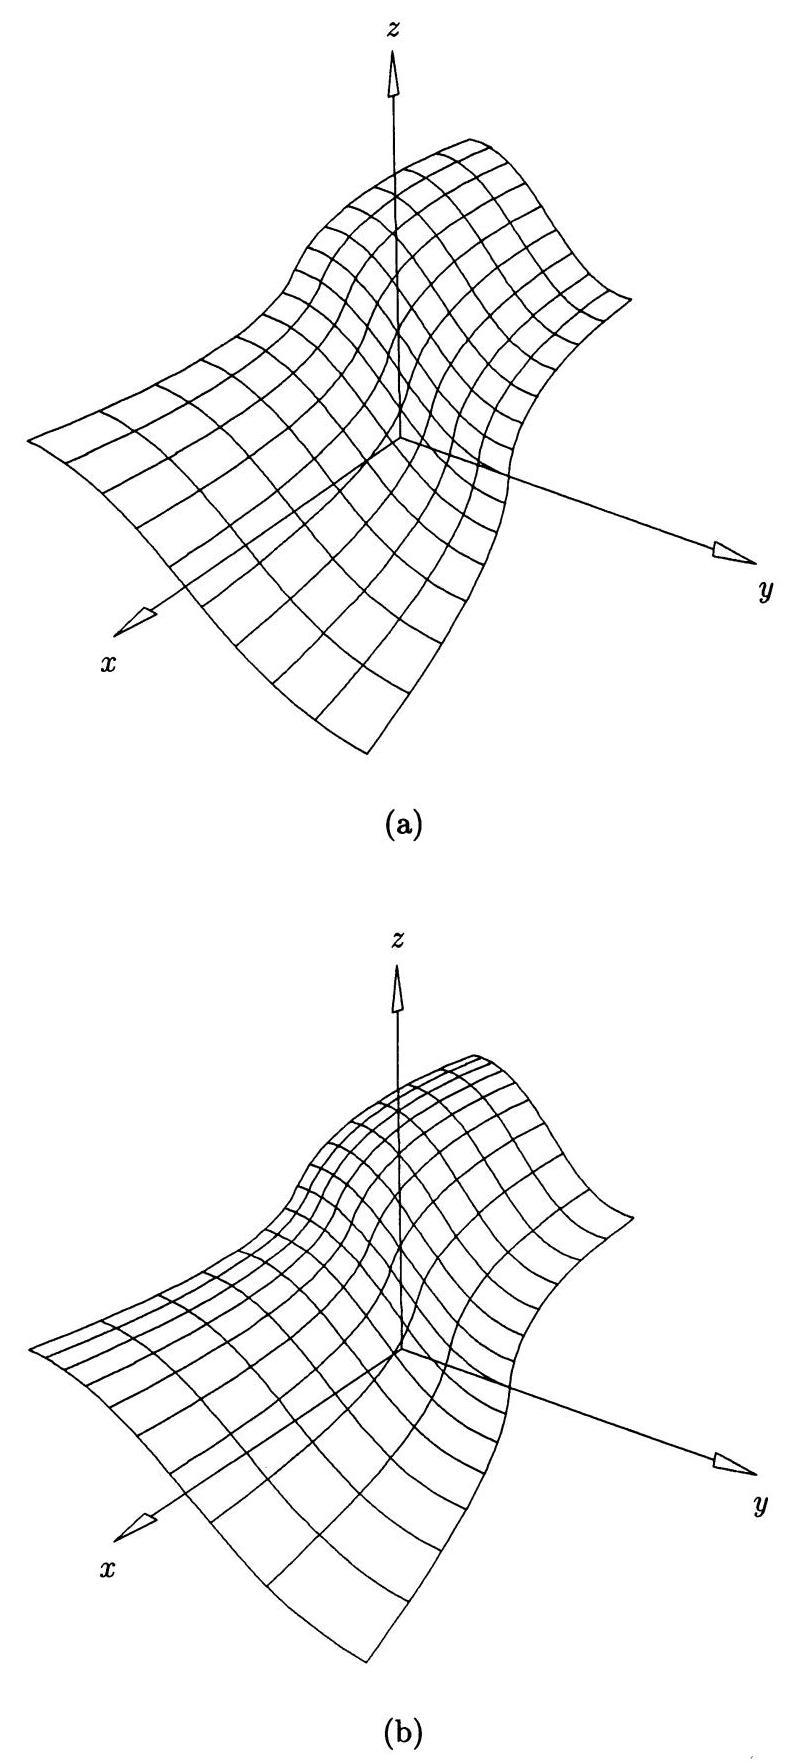
\includegraphics[max width=0.7\textwidth]{images/0193ba0d-ab19-7138-9798-cb281ce60de0_268_371_238_792_1761_0.jpg}
\end{center}
\hspace*{3em} 

图 6.14. 使用 \(g\left( u\right)  = {}^{\left( 2u + 1\right) }/{}_{\left( 3u + 2\right) }\) 的 NURBS 表面的有理重新参数化。(a) 原始表面；(b) 在 \(u\) 方向上的重新参数化；(c) 在 \(v\) 方向上的重新参数化；(d) 在两个方向上的重新参数化。

\begin{center}
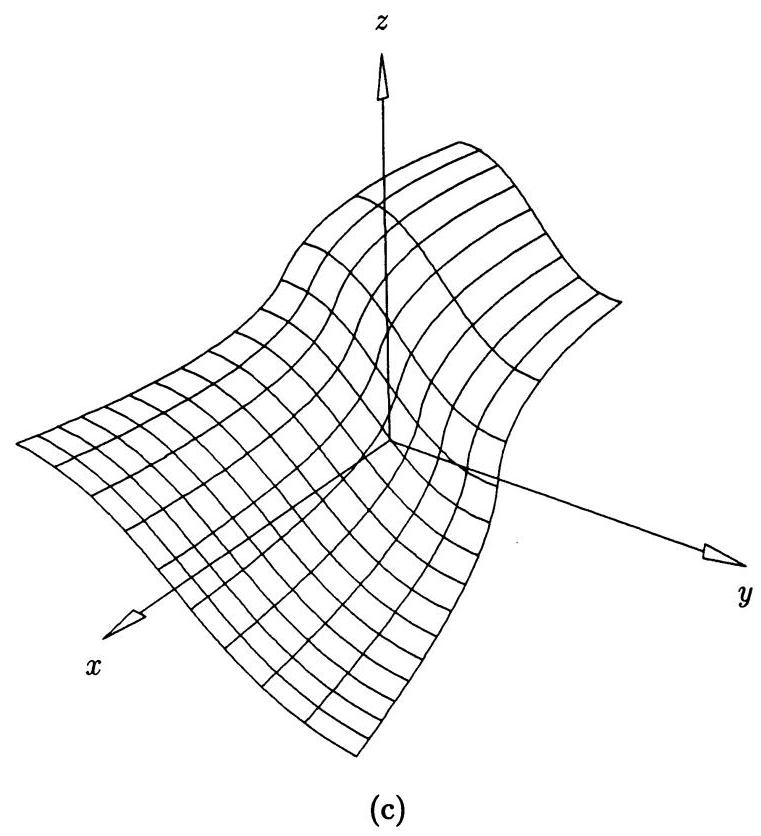
\includegraphics[max width=0.6\textwidth]{images/0193ba0d-ab19-7138-9798-cb281ce60de0_269_388_257_761_836_0.jpg}
\end{center}
\hspace*{3em} 

图 6.14. (续)

图 6.14c 在 \(v\) 方向上，图 6.14d 在两个方向上。注意图 \({6.14}\mathrm{\;b} - {6.14}\mathrm{\;d}\) 中参数线的分布不均匀。

现在假设 \(\mathbf{C}\left( u\right)\) 的末端权重不相等，即 \({w}_{0} \neq  {w}_{n}\) 。由于线性有理函数 \(s = g\left( u\right)\) 有三个自由度，因此应该能够确定满足三个条件的 \(g\left( u\right)\) 。

\[
c = g\left( a\right) \;d = g\left( b\right) \;{\bar{w}}_{0} = {\bar{w}}_{n}
\]

Lee 和 Lucian [Lee91] 推导出满足这些条件的函数。

\[
s = g\left( u\right)  = \frac{\sqrt[p]{{w}_{0}}\left( {b - u}\right) c + \sqrt[p]{{w}_{n}}\left( {u - a}\right) d}{\sqrt[p]{{w}_{0}}\left( {b - u}\right)  + \sqrt[p]{{w}_{n}}\left( {u - a}\right) } \tag{6.58}
\]

图 6.15 显示了一个重新参数化的例子，以使端权重相等。原始的三次 NURBS 曲线由以下定义

\[
U = \left\{  {0,0,0,0,\frac{3}{10},\frac{7}{10},1,1,1,1}\right\}  \;W = \{ 2,8,3,4,2,5\}
\]

选择的新区间为 \(\left\lbrack  {c,d}\right\rbrack   = \left\lbrack  {1/{10},4/5}\right\rbrack\) 。由公式 (6.58) 计算的重新参数化函数为

\[
g\left( u\right)  = \frac{{1.242u} + {0.126}}{{0.45u} + {1.26}}
\]

产生新的节点和权重

\[
{U}^{\prime } = \{ {0.1},{0.1},{0.1},{0.1},{0.36},{0.63},{0.8},{0.8},{0.8},{0.8}\}
\]

\[
{W}^{\prime } = \{ 1,{3.61},{1.08},{1.06},{0.43},1\}
\]

\begin{center}
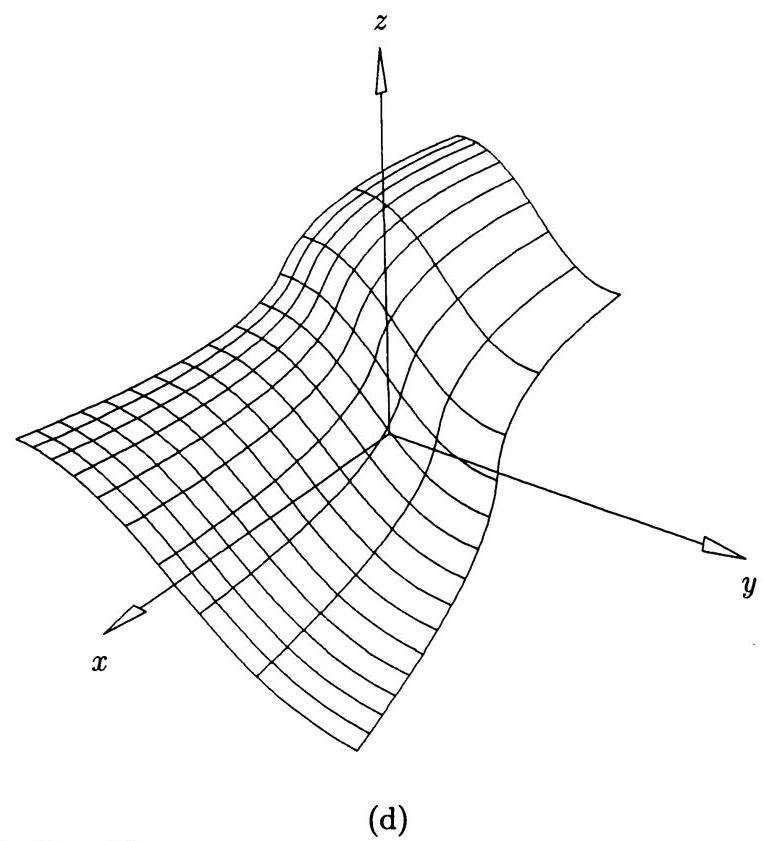
\includegraphics[max width=0.7\textwidth]{images/0193ba0d-ab19-7138-9798-cb281ce60de0_270_388_256_763_841_0.jpg}
\end{center}
\hspace*{3em} 

图 6.14. (续)

其中端权重被选择为 1。同样，+ 标记原始参数化，而 \(\square\) 标记新的参数化。

我们在第 4 章中给出了例子，表明权重的任意变化通常会改变有理 NURBS 曲线的形状(例如，见图 4.2 和 4.4)。在本节中，我们在不修改曲线形状的情况下改变了权重，唯一的变化是曲线的参数化。这表明，对于给定的曲线，权重之间必定存在一种关系来决定曲线形状，即保持这种关系的权重变化会导致曲线的重新参数化，而不会改变形状。这些关系被称为形状不变量或形状因子。对于有理 Bézier 曲线，它们仅依赖于次数；对于 NURBS 曲线，它们依赖于次数和节点。一般来说，这些形状不变量的推导相当复杂(见 [Forr68; Vers75; Patt85; Lee87; Pieg91a])。我们在此提供一些供参考； \({c}_{i}\) 表示常数。

\begin{itemize}
\item 二次 Bézier 曲线(圆锥曲线):
\end{itemize}

\[
\frac{{w}_{0}{w}_{2}}{{w}_{1}^{2}} = {c}_{1} \tag{6.59}
\]

\begin{center}
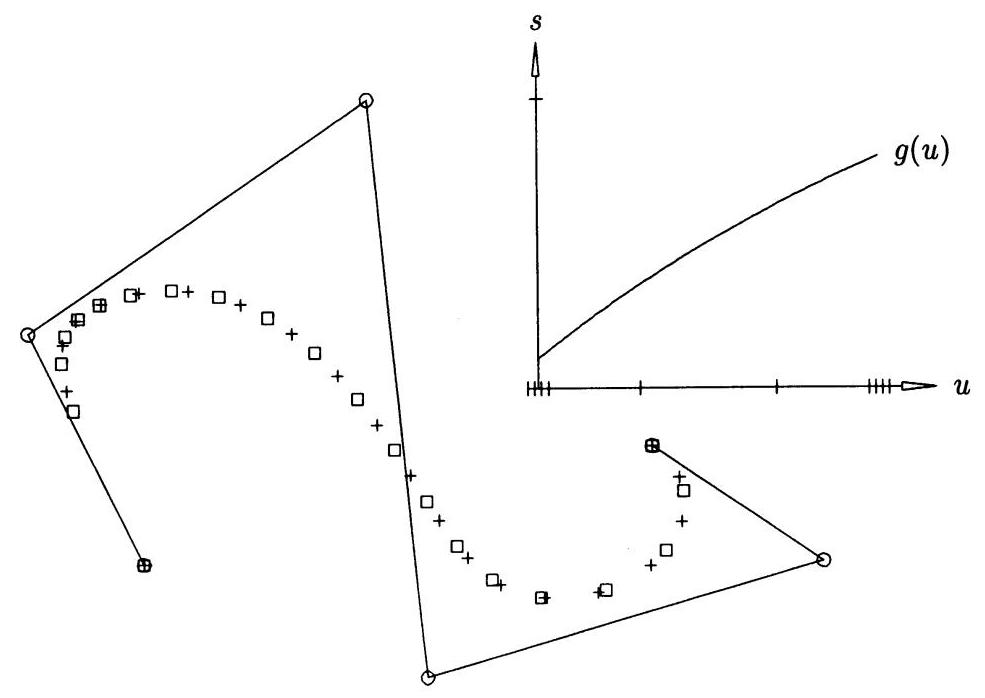
\includegraphics[max width=0.9\textwidth]{images/0193ba0d-ab19-7138-9798-cb281ce60de0_271_276_252_985_698_0.jpg}
\end{center}
\hspace*{3em} 

图 6.15. 曲线重新参数化以使端权重相等。

考虑圆弧，由 \(\left\{  {w}_{i}\right\}   = \{ 1,1,2\}\) (图 1.19b)或 \(\left\{  {w}_{i}\right\}   = \left\{  {1,\sqrt{2}/2,1}\right\}\) (公式 [6.55])定义

\[
2 = \frac{\left( 1\right) \left( 2\right) }{{1}^{2}} = \frac{\left( 1\right) \left( 1\right) }{{\left( \frac{\sqrt{2}}{2}\right) }^{2}} = 2
\]

假设控制点固定，任何三个权重代入公式 (6.59) 得到值 2 将产生圆弧；

\begin{itemize}
\item 三次 Bézier 曲线:
\end{itemize}

\[
\frac{{w}_{0}{w}_{2}}{{w}_{1}^{2}} = {c}_{1}\;\frac{{w}_{1}{w}_{3}}{{w}_{2}^{2}} = {c}_{2} \tag{6.60}
\]

\begin{itemize}
\item 一个 \(p\) 次贝塞尔曲线:
\end{itemize}

\[
\frac{{w}_{0}{w}_{2}}{{w}_{1}^{2}} = {c}_{1},\ldots ,\frac{{w}_{p - 2}{w}_{p}}{{w}_{p - 1}^{2}} = {c}_{p - 1} \tag{6.61}
\]

\begin{itemize}
\item 二次 NURBS 曲线 \({\mathbf{C}}^{w}\left( u\right)  = \mathop{\sum }\limits_{{i = 0}}^{n}{N}_{i,2}\left( u\right) {\mathbf{P}}_{i}^{w}\) 在 \(U = \left\{  {{u}_{0},\ldots ,{u}_{m}}\right\}\) 上:
\end{itemize}

\[
\frac{\left( {{u}_{i + 2} - {u}_{i + 1}}\right) {w}_{i - 1} + \left( {{u}_{i + 1} - {u}_{i}}\right) {w}_{i}}{\left( {{u}_{i + 3} - {u}_{i + 1}}\right) \left( {{u}_{i + 2} - {u}_{i}}\right) {w}_{i}^{2}} \times
\]

\[
\frac{\left( {{u}_{i + 3} - {u}_{i + 2}}\right) {w}_{i} + \left( {{u}_{i + 2} - {u}_{i + 1}}\right) {w}_{i + 1}}{\left( {{u}_{i + 3} - {u}_{i + 1}}\right) \left( {{u}_{i + 2} - {u}_{i}}\right) {w}_{i}^{2}} = {c}_{i} \tag{6.62}
\]

对于 \(i = 1,\ldots ,n - 1\) 。

我们以提及另一种有趣的技术来结束曲线的重新参数化。Fuhr 和 Kallay [Fuhr92] 开发了一种使用 \({C}^{1}\) 连续分段线性有理函数插值一组函数值的技术。他们的方法可以用来获得 \({C}^{1}\) 连续重新参数化，这不会提高次数，但可以映射任意多个内部点， \({u}_{i} = f\left( {s}_{i}\right)\) 。

NURBS 曲面 \(\;{\mathbf{S}}^{w}\left( {u,v}\right)  = \mathop{\sum }\limits_{{i = 0}}^{n}\mathop{\sum }\limits_{{j = 0}}^{m}{N}_{i,\;p}\left( u\right) {N}_{j,\;q}\left( v\right) {\mathbf{P}}_{i,j}^{w}\;\) 可以在 \(u\) 、 \(v\) 或两个方向上重新参数化。例如，它可以通过将 \(u\) 节点映射到 \(s\) 节点(方程 [6.51] 和 [6.52])在 \(u\) 方向上用多项式函数重新参数化，并将方程 (6.39) 到 (6.44) 应用于控制点的 \(m + 1\) 列。



\section{曲线和曲面的反转}

在本节中，我们使用重新参数化来反转 NURBS 曲线的方向和曲面法向量的方向。

设 \({\mathbf{C}}^{w}\left( u\right)  = \mathop{\sum }\limits_{{i = 0}}^{n}{N}_{i,p}\left( u\right) {\mathbf{P}}_{i}^{w}\) 是在 \(u \in  \left\lbrack  {a,b}\right\rbrack\) 上的 NURBS 曲线，且 \(u = f\left( s\right)\) 是在 \(s \in  \left\lbrack  {c,d}\right\rbrack\) 上的重新参数化函数。在第 6.4 节中，我们假设 \({f}^{\prime }\left( s\right)  > 0\) 在 \(s \in  \left\lbrack  {c,d}\right\rbrack\) 上。这在示例 Ex6.6 和方程 (6.41) 到 (6.44) 以及方程 (6.49) 的推导中隐含使用。

如果我们假设 \({f}^{\prime }\left( s\right)  < 0\) 在 \(s \in  \left\lbrack  {c,d}\right\rbrack\) 上，6.4 节的概念仍然适用。特别地，设

\[
u = f\left( s\right)  =  - s + a + b\;s \in  \left\lbrack  {a,b}\right\rbrack   \tag{6.63}
\]

注意到

\[
b = f\left( a\right) \;a = f\left( b\right)  \tag{6.64}
\]

并且 \({f}^{\prime }\left( s\right)  =  - 1\) 在 \(s \in  \left\lbrack  {a,b}\right\rbrack\) 上。 \(f\left( s\right)\) 的逆是

\[
s = g\left( u\right)  =  - u + a + b \tag{6.65}
\]

从 Eq. (6.53) 开始， \({\mathbf{C}}^{w}\left( s\right)\) 的节点通过计算得出

\[
{s}_{m - p - i} =  - {u}_{p + i} + a + b\;i = 1,\ldots ,m - {2p} - 1 \tag{6.66}
\]

其中 \({u}_{i}\) 是 \({\mathbf{C}}^{w}\left( u\right) ,0 \leq  i \leq  m\) 的节点。例如，如果 \(U = \{ 0,0,0,1,3,6\) ， \(6,8,8,8\}\) ，那么 \(S = \{ 0,0,0,2,2,5,7,8,8,8\}\) 。

\({\mathbf{C}}^{w}\left( s\right)\) 的控制点 \({\mathbf{Q}}_{i}^{w}\) 被计算为

\[
{\mathbf{Q}}_{0}^{w} = {\mathbf{C}}^{w}\left( {f\left( {s = a}\right) }\right)  = {\mathbf{C}}^{w}\left( {u = b}\right)  = {\mathbf{P}}_{n}^{w}
\]

\[
{\mathbf{Q}}_{1}^{w} = \frac{{s}_{p + 1} - a}{p}{\mathbf{C}}^{w\left( 1\right) }\left( {s = a}\right)  + {\mathbf{Q}}_{0}^{w}
\]

\[
= \frac{b - {u}_{m - p - 1}}{p}{\mathbf{C}}^{w\left( 1\right) }\left( {u = b}\right) {f}^{\prime }\left( {s = a}\right)  + {\mathbf{P}}_{n}^{w}
\]

\[
= \frac{b - {u}_{m - p - 1}}{p}\frac{p}{b - {u}_{m - p - 1}}\left( {{\mathbf{P}}_{n}^{w} - {\mathbf{P}}_{n - 1}^{w}}\right) \left( {-1}\right)  + {\mathbf{P}}_{n}^{w}
\]

\[
= {\mathbf{P}}_{n - 1}^{w}
\]

一般来说

\[
{\mathbf{Q}}_{i}^{w} = {\mathbf{P}}_{n - i}^{w} \tag{6.67}
\]

方程 (6.63)-(6.67) 的效果是反转曲线的方向。这在图 6.16 中显示；注意参数化没有改变。

设 \({\textbf{S}}^{w}\left( {u,v}\right)  = \mathop{\sum }\limits_{{i = 0}}^{n}\mathop{\sum }\limits_{{j = 0}}^{m}{N}_{i,\;p}\left( u\right) {N}_{j,\;q}\left( v\right) {\textbf{P}}_{i,j}^{w}\) 为具有节点向量 \(U = \left\{  {{u}_{0},\ldots ,{u}_{r}}\right\}\) 和 \(V = \left\{  {{v}_{0},\ldots ,{v}_{s}}\right\}\) 的 NURBS 曲面。曲面的参数化也可以被反转。更具体地说， \(u\) 的反转产生

\[
{\mathbf{S}}^{w}\left( {s,v}\right)  = \mathop{\sum }\limits_{{i = 0}}^{n}\mathop{\sum }\limits_{{j = 0}}^{m}{N}_{i,p}\left( s\right) {N}_{j,q}\left( v\right) {\mathbf{Q}}_{i,j}^{w} \tag{6.68}
\]

在 \(S\) 和 \(V\) 上，其中

\[
{s}_{r - p - i} =  - {u}_{p + i} + {u}_{0} + {u}_{r}\;i = 1,\ldots ,r - {2p} - 1 \tag{6.69}
\]

和

\[
{\mathbf{Q}}_{i,j}^{w} = {\mathbf{P}}_{n - i,j}^{w}\;i = 0,\ldots ,n\;j = 0,\ldots ,m \tag{6.70}
\]

类似地， \(v\) 的反转产生

\[
{\mathbf{S}}^{w}\left( {u,t}\right)  = \mathop{\sum }\limits_{{i = 0}}^{n}\mathop{\sum }\limits_{{j = 0}}^{m}{N}_{i,p}\left( u\right) {N}_{j,q}\left( t\right) {\mathbf{Q}}_{i,j}^{w} \tag{6.71}
\]

在 \(U\) 和 \(T\) 上，其中

\[
{t}_{s - q - j} =  - {v}_{q + j} + {v}_{0} + {v}_{s}\;j = 1,\ldots ,s - {2q} - 1 \tag{6.72}
\]

和

\[
{\mathbf{Q}}_{i,j}^{w} = {\mathbf{P}}_{i,m - j}^{w}\;i = 0,\ldots ,n\;j = 0,\ldots ,m \tag{6.73}
\]

\begin{center}
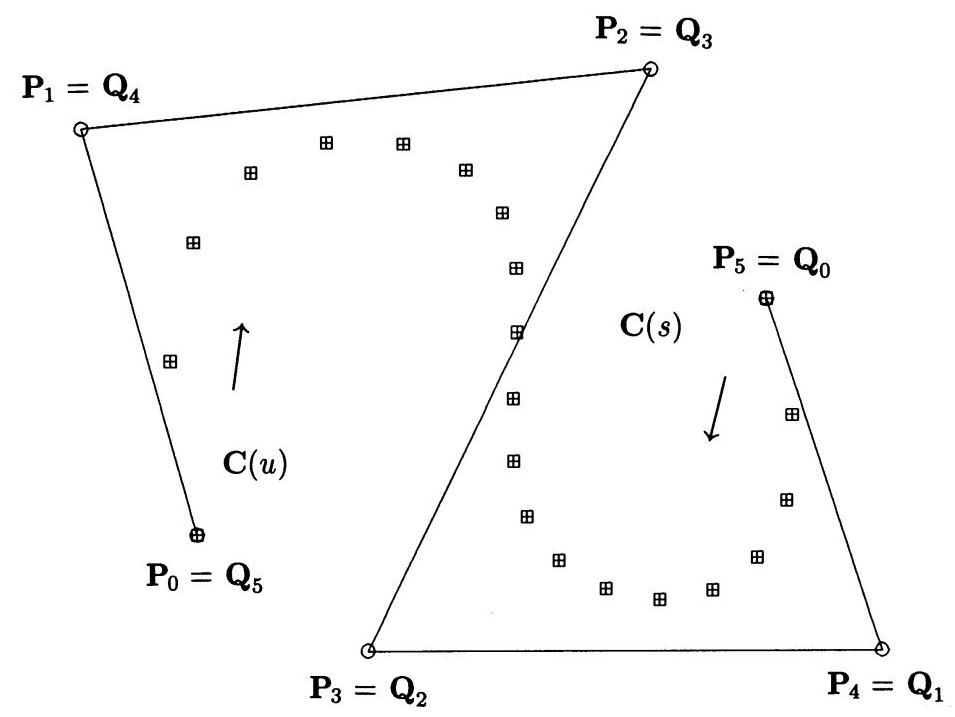
\includegraphics[max width=0.8\textwidth]{images/0193ba0d-ab19-7138-9798-cb281ce60de0_273_281_1365_955_717_0.jpg}
\end{center}
\hspace*{3em} 

图 6.16. 曲线反转；没有参数化变化发生。

在任意参数点 (u, v) 处，表面法向量由以下公式给出

\[
\mathbf{N}\left( {u,v}\right)  = {\mathbf{S}}_{u}\left( {u,v}\right)  \times  {\mathbf{S}}_{v}\left( {u,v}\right)  \tag{6.74}
\]

显然，通过反转 \({\mathbf{S}}_{u}\left( {u,v}\right)\) 或 \({\mathbf{S}}_{v}\left( {u,v}\right)\) (但不能同时反转)可以反转 \(\mathbf{N}\left( {u,v}\right)\) 的方向。这是通过分别应用方程 (6.68)-(6.70) 或方程 (6.71)-(6.73) 来实现的。

图 \({6.17}\mathrm{a} - {6.17}\mathrm{c}\) 显示了表面反转的示例。在图 \({6.17}\mathrm{a}\) 中，显示了原始度 \(\left( {3 \times  2}\right)\) 表面，以及 \({\mathbf{S}}_{u},{\mathbf{S}}_{v}\) 和 \(\mathbf{N}\) 。在图 \({6.17}\mathrm{\;b}\) 和 6.17c 中，参数化在 \(u\) 和 \(v\) 方向上被反转。注意，在每种情况下法向量都被反转。



\section{B-spline 和分段幂基形式之间的转换}

将 B-spline 曲线或表面转换为分段幂基形式的步骤如下:

1. 使用节点细化，例如算法 A5.4-A5.7，将曲线或表面分解为分段 Bézier 形式；

2. 通过应用矩阵乘法(基变换)将每个 Bézier 曲线段(或表面片)转换为幂基形式；

3. 应用矩阵乘法对步骤 2 中获得的幂基形式进行重新参数化。

像往常一样，所有方程都应用于四维控制点和幂基系数；为方便起见，我们省略所有 \(w\) 上标。步骤 1 无需进一步阐述。

假设第 \(j\) 条曲线段 \({\mathbf{C}}_{j}\left( u\right)\) 定义在 \(u \in  \left\lbrack  {{u}_{j},{u}_{j + 1}}\right\rbrack\) 上。现在，在步骤 1 中为 \({\mathbf{C}}_{j}\left( u\right)\) 获得的 Bézier 控制点 \({\mathbf{P}}_{i},i = 0,\ldots ,p\) 是有效的，但我们对 Bézier 曲线的定义要求有 \(\left\lbrack  {0,1}\right\rbrack\) 参数化(方程 [1.7] 和 [1.8])。设

\[
u = \left( {{u}_{j + 1} - {u}_{j}}\right) s + {u}_{j} \tag{6.75}
\]

然后 \(0 \leq  s \leq  1\) ，第 \(j\) 段具有 Bézier 形式

\[
{\mathbf{C}}_{j}\left( s\right)  = \mathop{\sum }\limits_{{i = 0}}^{p}{B}_{i,p}\left( s\right) {\mathbf{P}}_{i} = {\left\lbrack  {B}_{i,p}\left( s\right) \right\rbrack  }^{T}\left\lbrack  {\mathbf{P}}_{i}\right\rbrack   = {\left\lbrack  {s}^{i}\right\rbrack  }^{T}{M}_{p}\left\lbrack  {\mathbf{P}}_{i}\right\rbrack   \tag{6.76}
\]

其中 \({\left\lbrack  {B}_{i,p}\left( s\right) \right\rbrack  }^{T}\) 和 \({\left\lbrack  {s}^{i}\right\rbrack  }^{T}\) 是 \(1 \times  \left( {p + 1}\right)\) 行向量的标量值， \({M}_{p}\) 是标量的 \(\left( {p + 1}\right)  \times  \left( {p + 1}\right)\) 矩阵， \(\left\lbrack  {\mathbf{P}}_{i}\right\rbrack\) 是四维点的 \(\left( {p + 1}\right)  \times  1\) 列向量。设定

\[
\left\lbrack  {\mathbf{a}}_{i}\right\rbrack   = {M}_{p}\left\lbrack  {\mathbf{P}}_{i}\right\rbrack   \tag{6.77}
\]

我们得到

\[
{\mathbf{C}}_{j}\left( s\right)  = {\left\lbrack  {s}^{i}\right\rbrack  }^{T}\left\lbrack  {\mathbf{a}}_{i}\right\rbrack   \tag{6.78}
\]

266 高级几何算法

\begin{center}
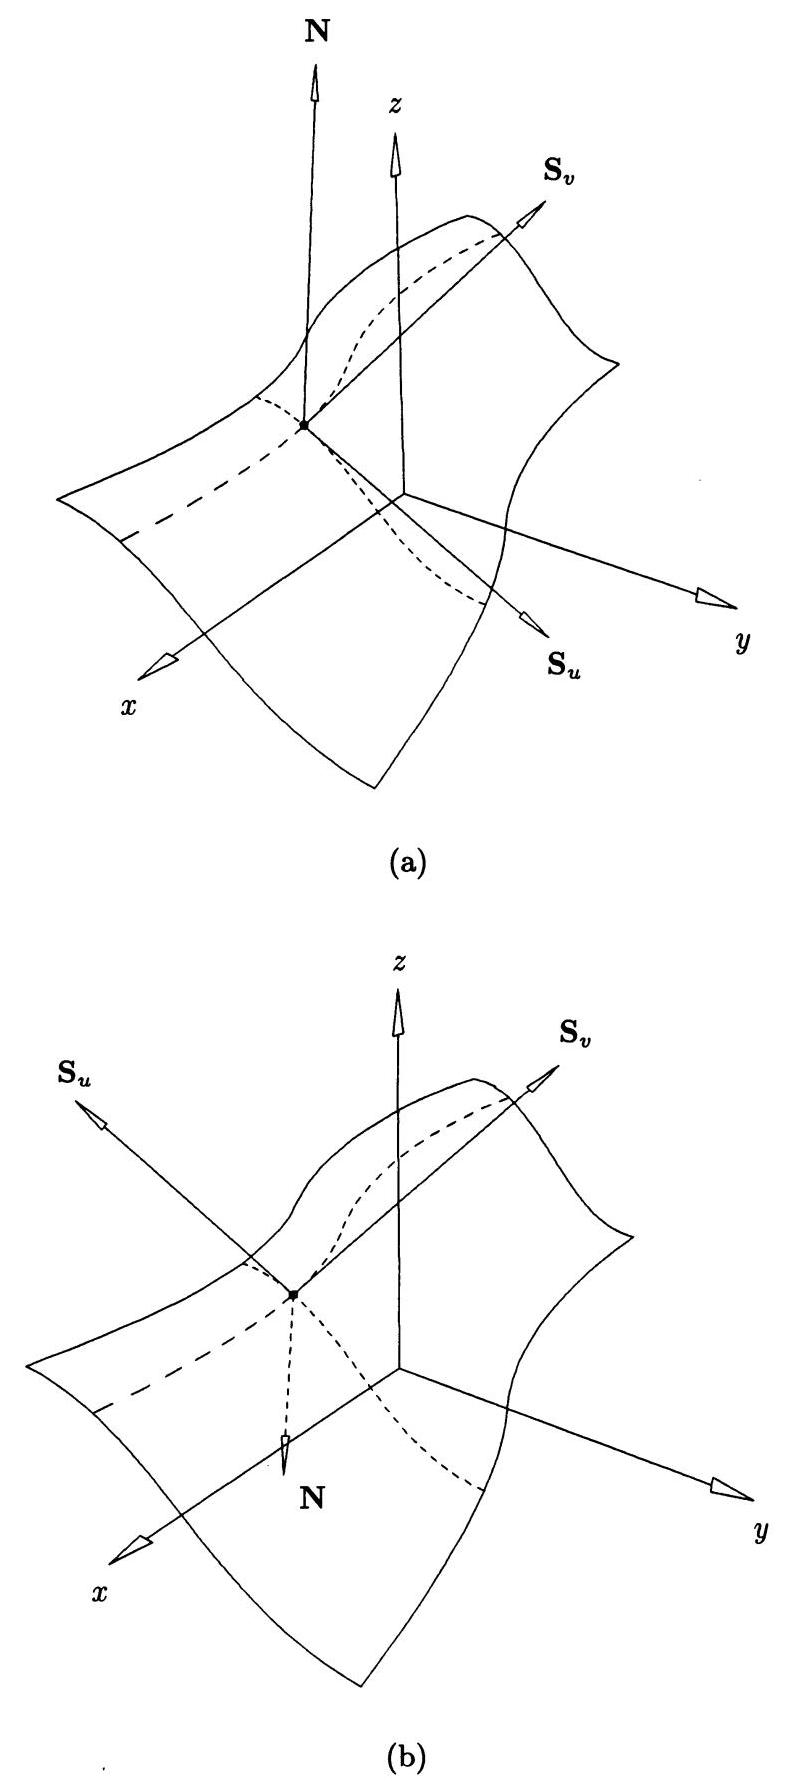
\includegraphics[max width=0.7\textwidth]{images/0193ba0d-ab19-7138-9798-cb281ce60de0_275_369_239_785_1786_0.jpg}
\end{center}
\hspace*{3em} 

图 6.17. 表面反转。(a) 原始表面显示偏导数和法向量；(b) 在 \(u\) 方向上反转参数化；(c) 在 \(v\) 方向上反转参数化。

\begin{center}
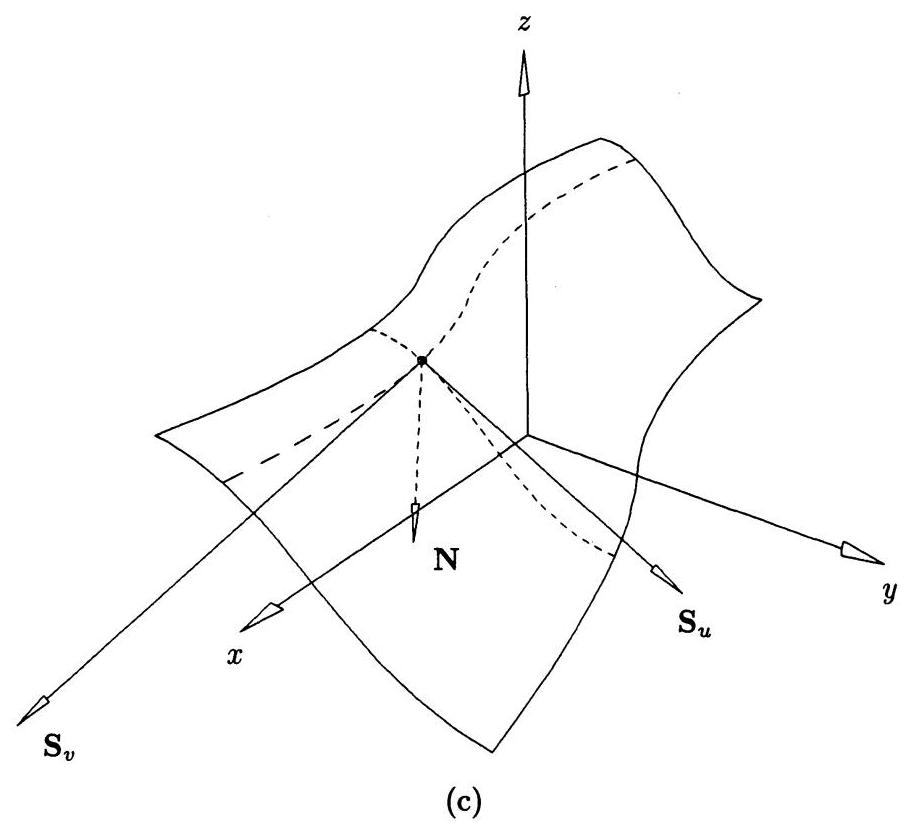
\includegraphics[max width=0.8\textwidth]{images/0193ba0d-ab19-7138-9798-cb281ce60de0_276_309_259_907_828_0.jpg}
\end{center}
\hspace*{3em} 

图 6.17.(续)

这是参数 \(s\) 中第 \(j\) 段的幂基形式。

现在我们推导任意 \(p\) 的矩阵 \({M}_{p}\) 。作为热身和参考，我们计算前三个矩阵。从方程 (6.76) 可以得出

\[
{\left\lbrack  {B}_{i,p}\left( s\right) \right\rbrack  }^{T} = {\left\lbrack  {s}^{i}\right\rbrack  }^{T}{M}_{p} \tag{6.79}
\]

对于 \(p = 1,2,3\) ，从方程 (1.8) 中，我们得到

\[
\left\lbrack  \begin{array}{ll} 1 - s & s \end{array}\right\rbrack   = \left\lbrack  \begin{array}{ll} 1 & s \end{array}\right\rbrack  \left\lbrack  \begin{matrix} 1 & 0 \\   - 1 & 1 \end{matrix}\right\rbrack
\]

\[
\left\lbrack  \begin{array}{lll} {\left( 1 - s\right) }^{2} & {2s}\left( {1 - s}\right) & {s}^{2} \end{array}\right\rbrack   = \left\lbrack  \begin{array}{lll} 1 & s & {s}^{2} \end{array}\right\rbrack  \left\lbrack  \begin{matrix} 1 & 0 & 0 \\   - 2 & 2 & 0 \\  1 &  - 2 & 1 \end{matrix}\right\rbrack
\]

\[
\left\lbrack  \begin{array}{llll} {\left( 1 - s\right) }^{3} & {3s}{\left( 1 - s\right) }^{2} & 3{s}^{2}\left( {1 - s}\right) & {s}^{3} \end{array}\right\rbrack   = \left\lbrack  \begin{array}{llll} 1 & s & {s}^{2} & {s}^{3} \end{array}\right\rbrack  \left\lbrack  \begin{matrix} 1 & 0 & 0 & 0 \\   - 3 & 3 & 0 & 0 \\  3 &  - 6 & 3 & 0 \\   - 1 & 3 &  - 3 & 1 \end{matrix}\right\rbrack
\]

(6.80)

现在我们推导一般公式。设 \({M}_{p}\left( {i,j}\right)\) 表示 \({M}_{p}\) 中第 \(i\) 行和第 \(j\) 列的元素。从方程 (1.8) 中我们有

\[
{\left( 1 - s\right) }^{p} = \left( \begin{array}{l} p \\  0 \end{array}\right) {s}^{0}{\left( 1 - s\right) }^{p} = {B}_{0,p}\left( s\right)  = {\left\lbrack  {s}^{i}\right\rbrack  }^{T}\left\lbrack  {{M}_{p}\left( {i,0}\right) }\right\rbrack
\]

\[
= \left\lbrack  \begin{array}{llll} 1 & s & \cdots & {s}^{p} \end{array}\right\rbrack  \left\lbrack  \begin{matrix} {M}_{p}\left( {0,0}\right) \\  \vdots \\  {M}_{p}\left( {p,0}\right)  \end{matrix}\right\rbrack
\]

从初等代数来看，展开 \({\left( 1 - s\right) }^{p}\) 产生带有交替符号的二项式系数；因此

\[
{M}_{p}\left( {i,0}\right)  = {\left( -1\right) }^{i}\left( \begin{matrix} p \\  i \end{matrix}\right) \;i = 0,\ldots ,p \tag{6.81}
\]

一般来说， \(k\) 列的 \({M}_{p}\) 定义为

\[
\left( \begin{array}{l} p \\  k \end{array}\right) {s}^{k}{\left( 1 - s\right) }^{p - k} = {B}_{k,p}\left( s\right)  = {\left\lbrack  {s}^{i}\right\rbrack  }^{T}\left\lbrack  {{M}_{p}\left( {i,k}\right) }\right\rbrack
\]

检查 \(\left( \begin{array}{l} p \\  k \end{array}\right) {s}^{k}{\left( 1 - s\right) }^{p - k}\) 显示

\begin{itemize}
\item 展开项 \({\left( 1 - s\right) }^{p - k}\) 产生二项式系数
\end{itemize}

\[
{\left( -1\right) }^{j}\left( \begin{matrix} p - k \\  j \end{matrix}\right) \;j = 0,\ldots ,p - k
\]

\begin{itemize}
\item 乘以 \({s}^{k}\) 会导致 \({M}_{p}\left( {j,k}\right)  = 0\) 对于 \(j = 0,\ldots ,k - 1\) ，并且上面的值向下移动了 \(k\) 行；
\end{itemize}

\begin{itemize}
\item \(k\) 列的所有元素都乘以 \(\left( \begin{array}{l} p \\  k \end{array}\right)\) 。
\end{itemize}

总之，对于 \(k = 0,\ldots ,p\) ， \(k\) 列的 \({M}_{p}\) 由以下给出

\[
{M}_{p}\left( {j,k}\right)  = \left\{  \begin{matrix} 0 & j = 0,\ldots ,k - \\  {\left( -1\right) }^{j - k}\left( \begin{array}{l} p \\  k \end{array}\right) \left( \begin{array}{l} p - k \\  j - k \end{array}\right) & j = k,\ldots ,p \end{matrix}\right.  \tag{6.82}
\]

我们将其留作练习以证明

\[
{M}_{p}\left( {j,k}\right)  = {M}_{p}\left( {p - k,p - j}\right)  \tag{6.83}
\]

注意矩阵 \({M}_{p}\) 的附加属性:

\begin{itemize}
\item 对角元素是度数为 \(p\) 的二项式系数；
\end{itemize}

\begin{itemize}
\item 最后一行和第一列中的元素也是度数为 \(p\) 的二项式系数，但符号交替；
\end{itemize}

\begin{itemize}
\item 每行和每列的元素之和为一。方程 (6.83) 表示 \({M}_{p}\) 关于从左下角元素到右上角元素的对角线是对称的。
\end{itemize}

算法 A6.1 高效地计算 \({M}_{p}\) 。一个数组 bin[i][j]，它包含

\HRule

the precomputed binomial coefficients, is used.

\hspace*{3em} ALGORITHM A6.1

\hspace*{5em} BezierToPowerMatrix(p, M)

\hspace*{7em} \{ /* Compute pth degree Bézier matrix */

\hspace*{10em} /* Input: p */

\hspace*{10em} /* Output: M */

\hspace*{7em} for (i=0; i<p; i++) /* Set upper triangle to zero */

\hspace*{9em} for \(\left( {j = i + 1;j <  = p;j +  + }\right) \;M\left\lbrack  i\right\rbrack  \left\lbrack  j\right\rbrack   = {0.0}\) ;

\hspace*{7em} \(M\left\lbrack  0\right\rbrack  \left\lbrack  0\right\rbrack   = M\left\lbrack  p\right\rbrack  \left\lbrack  p\right\rbrack   = {1.0};/ *\) Set corner elements \(* /\)

\hspace*{7em} if (p mod 2) M[p][0] = -1.0;

\hspace*{9em} else M[p][0] = 1.0 ;

\hspace*{7em} sign = -1.0 ;

\hspace*{7em} for (i=1; i<p; i++) /* Compute first column, last row,*/

\hspace*{9em} /* and the diagonal */

\hspace*{9em} M[i][i] = bin[p][i];

\hspace*{9em} \(M\left\lbrack  i\right\rbrack  \left\lbrack  0\right\rbrack   = M\left\lbrack  p\right\rbrack  \left\lbrack  {p - i}\right\rbrack   = \operatorname{sign} * M\left\lbrack  i\right\rbrack  \left\lbrack  i\right\rbrack  ;\)

\hspace*{9em} sign = -sign;

\hspace*{9em} \}

\hspace*{7em} /* Compute remaining elements \(*\) /

\hspace*{7em} \(\mathrm{k}1 = \left( {\mathrm{p} + 1}\right) /2;\;\mathrm{{pk}} = \mathrm{p} - 1;\)

\hspace*{7em} for (k=1; k<k1; k++)

\hspace*{9em} \{

\hspace*{9em} sign = -1.0 ;

\hspace*{9em} for (j=k+1; j<=pk; j++)

\hspace*{11em} \{

\hspace*{11em} \(M\left\lbrack  j\right\rbrack  \left\lbrack  k\right\rbrack   = M\left\lbrack  {pk}\right\rbrack  \left\lbrack  {p - j}\right\rbrack   = \operatorname{sign} * \operatorname{bin}\left\lbrack  p\right\rbrack  \left\lbrack  k\right\rbrack   * \operatorname{bin}\left\lbrack  {p - k}\right\rbrack  \left\lbrack  {j - k}\right\rbrack  ;\)

\hspace*{11em} sign = -sign;

\hspace*{11em} \}

\hspace*{9em} \(\mathrm{{pk}} = \mathrm{{pk}} - 1\) ;

\hspace*{9em} \}

\hspace*{7em} \}

\HRule

现在我们进入将 B-spline 曲线转换为分段幂基的步骤 3，即重新参数化方程 (6.78) 以获得

\[
{\mathbf{C}}_{j}\left( u\right)  = {\left\lbrack  {u}^{i}\right\rbrack  }^{T}\left\lbrack  {\mathbf{b}}_{i}\right\rbrack   \tag{6.84}
\]

原参数中的幂基段 \(u\) 。我们将详细讨论 \(p = 2\) ，然后给出一般公式但不提供证明。解方程 (6.75) 得到 \(s\) 结果为

\[
s = \frac{1}{{u}_{j + 1} - {u}_{j}}u - \frac{{u}_{j}}{{u}_{j + 1} - {u}_{j}} = {cu} + d \tag{6.85}
\]

对于 \(p = 2\) ，将 \(s = {cu} + d\) 代入方程 (6.78) 并将结果与方程 (6.84) 相等，得到

\[
{\left\lbrack  {s}^{i}\right\rbrack  }^{T}\left\lbrack  {\mathbf{a}}_{i}\right\rbrack   = {\left\lbrack  {\left( cu + d\right) }^{i}\right\rbrack  }^{T}\left\lbrack  {\mathbf{a}}_{i}\right\rbrack   = {\left\lbrack  \begin{array}{lll} 1 & {cu} + d & {c}^{2}{u}^{2} + {2cdu} + {d}^{2} \end{array}\right\rbrack  }^{T}\left\lbrack  {\mathbf{a}}_{i}\right\rbrack
\]

\[
= \left\lbrack  \begin{array}{lll} 1 & u & {u}^{2} \end{array}\right\rbrack  R\left\lbrack  {\mathbf{a}}_{i}\right\rbrack   = \left\lbrack  \begin{array}{lll} 1 & u & {u}^{2} \end{array}\right\rbrack  \left\lbrack  {\mathbf{b}}_{i}\right\rbrack   \tag{6.86}
\]

其中

\[
R = \left\lbrack  \begin{matrix} 1 & d & {d}^{2} \\  0 & c & {2cd} \\  0 & 0 & {c}^{2} \end{matrix}\right\rbrack
\]

从方程 (6.86) 可以得出

\[
R\left\lbrack  {\mathbf{a}}_{i}\right\rbrack   = \left\lbrack  {\mathbf{b}}_{i}\right\rbrack   \tag{6.87}
\]

\(\left\lbrack  {\mathbf{b}}_{i}\right\rbrack\) 是所需的幂基系数。

一般来说，对于 \(s = {cu} + d\) ，第 \(p\) 次重参数化矩阵为

\[
{R}_{p} = \left\lbrack  {r}_{i,j}\right\rbrack
\]

其中

\[
{r}_{i,j} = \left\{  \begin{matrix} 0 & j < i \\  \left( \begin{matrix} j \\  i \end{matrix}\right) {c}^{i}{d}^{j - i} & i \leq  j\;i,j = 0,\ldots ,p \end{matrix}\right.  \tag{6.88}
\]

结合方程 (6.77) 和 (6.87)，我们得到

\[
\left\lbrack  {\mathbf{b}}_{i}\right\rbrack   = {R}_{p}{M}_{p}\left\lbrack  {\mathbf{P}}_{i}\right\rbrack   \tag{6.89}
\]

关于以 Bézier 控制点为基础的幂基系数。图 6.18 显示了 B-spline 到幂基转换的一个示例。一个具有三个段的三次 NURBS 曲线被转换为分段幂基形式。图 6.18 说明了曲线并标记了其第二段。请注意，该段由中间的四个控制点定义。中间曲线段也被显示，以及向量系数 \({\mathbf{b}}_{0},{\mathbf{b}}_{1},{\mathbf{b}}_{2}\) 和 \({\mathbf{b}}_{3}\) ，它们经过 \(1/{10}\) 的缩放以适应图形。请注意，向量系数与曲线没有几何关系。多项式片段定义在 \(\left\lbrack  {3/{10},7/{10}}\right\rbrack\) 上。

我们以两个最后的备注完成 B-spline 到幂基转换的讨论:

\begin{itemize}
\item IGES 参数样条(实体 112 和 114)[IGE93] 假设每个段的参数化从零开始；这意味着在方程 (6.85) 中 \(d = 0\) ，因此 \({R}_{p}\) 简化为具有元素的对角矩阵。
\end{itemize}

\[
{r}_{i,j} = \left\{  {\begin{array}{ll} 0 & i \neq  j \\  {c}^{i} & i = j \end{array}\;i = 0,\ldots ,p}\right.  \tag{6.90}
\]

\begin{center}
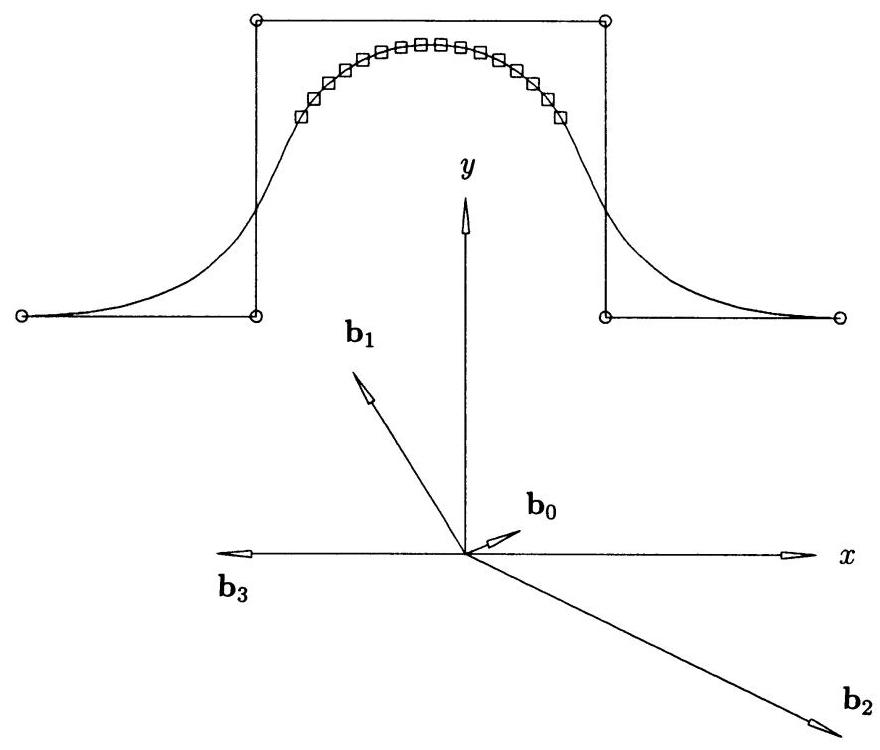
\includegraphics[max width=0.8\textwidth]{images/0193ba0d-ab19-7138-9798-cb281ce60de0_280_323_266_880_750_0.jpg}
\end{center}
\hspace*{3em} 

图 6.18. 将 NURBS 曲线转换为以幂基形式表示的分段多项式曲线。

\begin{itemize}
\item 对于曲面，方程 (6.89) 变为
\end{itemize}

\[
\left\lbrack  {\mathbf{b}}_{i,j}\right\rbrack   = {R}_{p}{M}_{p}\left\lbrack  {\mathbf{P}}_{i,j}\right\rbrack  {M}_{q}^{T}{R}_{q}^{T} \tag{6.91}
\]

其中 \({R}_{p}\) 和 \({R}_{q}^{T}\) 是重新参数化矩阵，将 \(u\) 转换为 \(s\) ，将 \(v\) 转换为 \(t\) ，分别 \(\left( {0 \leq  s,t \leq  1}\right)\) 。

图 6.19a 和 \({6.19}\mathrm{\;b}\) 显示了 B-spline 曲面到幂基转换。测试曲面是一个定义在 的度 \(\left( {3 \times  2}\right)\) 曲面。

\[
U = \left\{  {0,0,0,0,\frac{3}{10},\frac{7}{10},1,1,1,1}\right\}  \;V = \left\{  {0,0,0,\frac{3}{10},\frac{3}{5},1,1,1}\right\}
\]

图6.19a中显示了三个多项式补丁:在 \(\left\lbrack  {0,{\;}^{3}{/}_{10}}\right\rbrack   \times  \left\lbrack  {{\;}^{3}{/}_{5},1}\right\rbrack\) 上定义的patch(0,2)；在 \(\left\lbrack  {{\;}^{3}{/}_{10},{\;}^{7}{/}_{10}}\right\rbrack   \times  \left\lbrack  {{\;}^{3}{/}_{10},{\;}^{3}{/}_{5}}\right\rbrack\) 上定义的patch(1,1)；以及在 \(\left\lbrack  {7/{10},1}\right\rbrack   \times  \left\lbrack  {0,3/{10}}\right\rbrack\) 上定义的patch(2,0)。图6.19b展示了一些在幂基形式下定义patch(1,1)的向量系数。这些向量经过 \(1/2\) 缩放以便更好地可视化。请注意补丁几何形状与向量系数之间缺乏任何几何关系。将此图与第5章的图5.25进行比较。

现在我们讨论将分段幂基曲线或曲面转换为B样条形式的过程。步骤如下:

1. 应用矩阵乘法将幂基段(补丁)重新参数化到区间 \(\left\lbrack  {0,1}\right\rbrack\) ；

\begin{center}
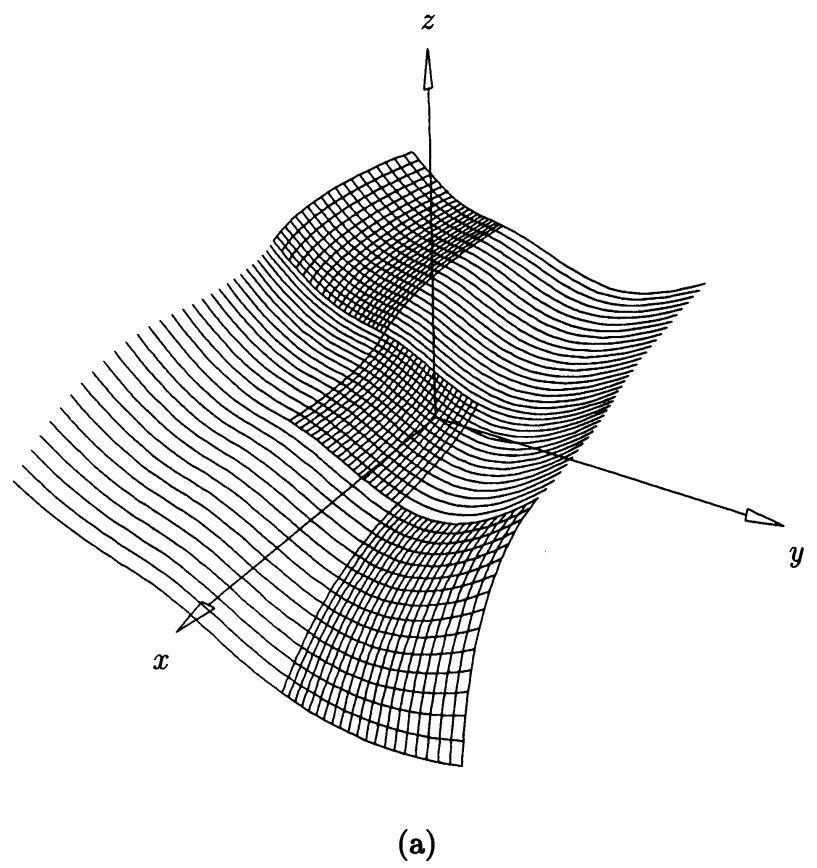
\includegraphics[max width=0.7\textwidth]{images/0193ba0d-ab19-7138-9798-cb281ce60de0_281_360_248_817_868_0.jpg}
\end{center}
\hspace*{3em} 

图6.19. 将NURBS曲面转换为以幂基形式表示的多项式补丁集合。(a) 显示了索引为 \(\left( {0,2}\right) ,\left( {1,1}\right)\) 和(2,0)的补丁；(b) 定义patch(1,1)的一些向量系数。

2. 应用矩阵乘法将每个幂基段(补丁)转换为Bézier形式；

3. 将各段(补丁)拼接在一起形成B样条曲线或曲面，所有内部节点的重数等于度数(如果不能假设 \({C}^{0}\) 连续性，则为度数加一)；节点的值由原始幂基段(补丁)的参数边界给出；

4. 使用节点移除以获得B样条曲线或曲面的最小表示(曲线的算法为A5.8，或参见[Till92]的曲面算法)。

第3步和第4步无需进一步阐述。首先考虑曲线。设

\[
{\mathbf{C}}_{j}\left( u\right)  = {\left\lbrack  {u}^{i}\right\rbrack  }^{T}\left\lbrack  {\mathbf{a}}_{i}\right\rbrack   \tag{6.92}
\]

是 \(j\) 次曲线段的幂基形式，具有 \(u \in  \left\lbrack  {{u}_{j},{u}_{j + 1}}\right\rbrack\) 。我们需要该段的相应 Bézier 形式

\[
{\mathbf{C}}_{j}\left( s\right)  = {\left\lbrack  {B}_{i,p}\left( s\right) \right\rbrack  }^{T}\left\lbrack  {\mathbf{P}}_{i}\right\rbrack   = {\left\lbrack  {s}^{i}\right\rbrack  }^{T}{M}_{p}\left\lbrack  {\mathbf{P}}_{i}\right\rbrack
\]

\[
= {\left\lbrack  \begin{array}{l} {u}^{i} \end{array}\right\rbrack  }^{T}{R}_{p}{M}_{p}\left\lbrack  {\mathbf{P}}_{i}\right\rbrack   = {\left\lbrack  \begin{array}{l} {u}^{i} \end{array}\right\rbrack  }^{T}\left\lbrack  {\mathbf{a}}_{i}\right\rbrack   = {\mathbf{C}}_{j}\left( u\right)
\]

其中 \(s \in  \left\lbrack  {0,1}\right\rbrack\) 。因此

\[
\left\lbrack  {\mathbf{a}}_{i}\right\rbrack   = {R}_{p}{M}_{p}\left\lbrack  {\mathbf{P}}_{i}\right\rbrack
\]

\begin{center}
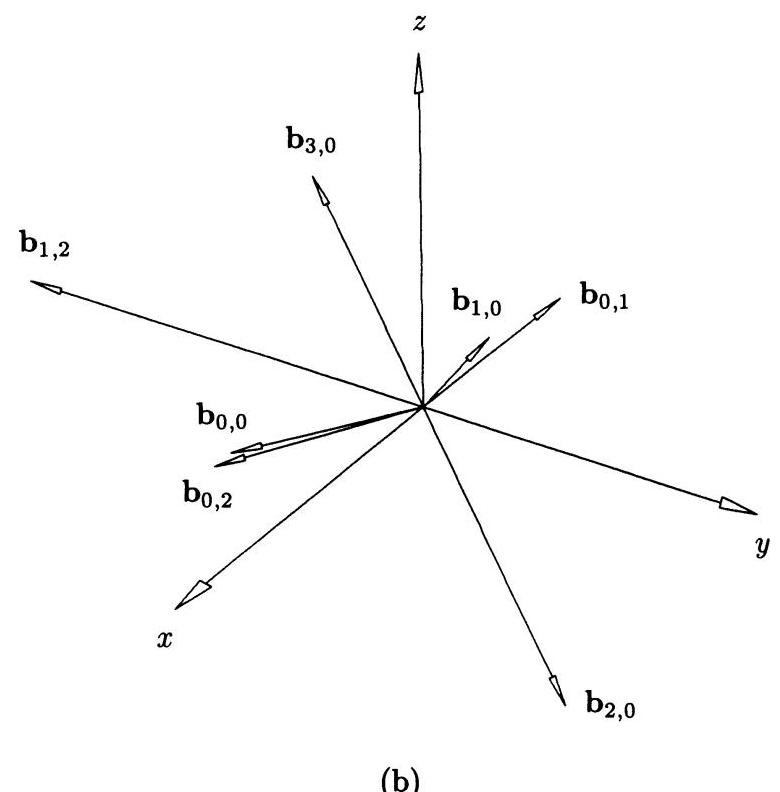
\includegraphics[max width=0.7\textwidth]{images/0193ba0d-ab19-7138-9798-cb281ce60de0_282_374_246_780_792_0.jpg}
\end{center}
\hspace*{3em} 

图 6.19. (续)

和

\[
\left\lbrack  {\mathbf{P}}_{i}\right\rbrack   = {M}_{p}^{-1}{R}_{p}^{-1}\left\lbrack  {\mathbf{a}}_{i}\right\rbrack   \tag{6.93}
\]

图 6.20a 到 6.20c 显示了幂基到 NURBS 转换的示例。图 6.20a 说明了在 \({s}_{0} < {s}_{1} <\)  \({s}_{2} < {s}_{3}\) 上定义的分段三次幂基曲线。在图 \({6.20}\mathrm{\;b}\) 中，每一段都被转换为 Bézier 形式，即它是具有三重内部节点的 B-spline 曲线。图 \({6.20}\mathrm{c}\) 显示了去除节点后的 B-spline 曲线。注意，原始曲线在 \({s}_{1}\) 处是 \({C}^{2}\) 连续的，但在 \({s}_{2}\) 处仅是 \({C}^{1}\) 连续的；因此， \({s}_{2}\) 是最终节点向量中的双重节点。很容易反转矩阵 \({M}_{1},{M}_{2}\) 和 \({M}_{3}\) ，如公式 (6.80) 所示，以获得

\[
{M}_{1}^{-1} = \left\lbrack  \begin{array}{ll} 1 & 0 \\  1 & 1 \end{array}\right\rbrack
\]

\[
{M}_{2}^{-1} = \left\lbrack  \begin{array}{lll} 1 & 0 & 0 \\  1 & \frac{1}{2} & 0 \\  1 & 1 & 1 \end{array}\right\rbrack
\]

274 高级几何算法

\[
{M}_{3}^{-1} = \left\lbrack  \begin{matrix} 1 & 0 & 0 & 0 \\  1 & \frac{1}{3} & 0 & 0 \\  1 & \frac{2}{3} & \frac{1}{3} & 0 \\  1 & 1 & 1 & 1 \end{matrix}\right\rbrack   \tag{6.94}
\]

\begin{center}
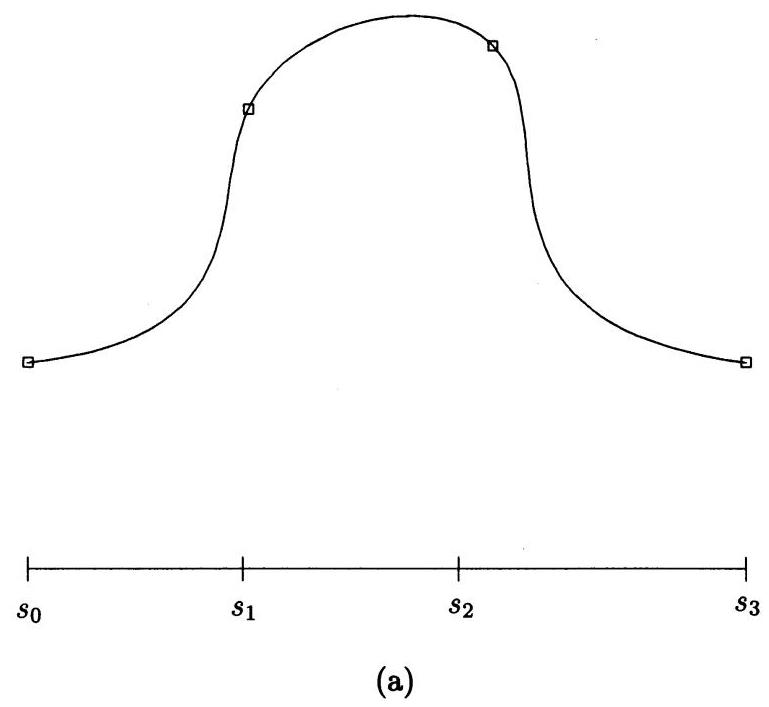
\includegraphics[max width=0.7\textwidth]{images/0193ba0d-ab19-7138-9798-cb281ce60de0_283_381_251_769_707_0.jpg}
\end{center}
\hspace*{3em} 

图 6.20. 将分段多项式曲线转换为 NURBS 形式。(a)在 \({s}_{0} < {s}_{1} < {s}_{2} < {s}_{3}\) 上定义的分段多项式；(b)将每一段转换为 Bézier 形式；(c)去除节点后的 NURBS 表示。

给定 \({M}_{p}\) ， \({M}_{p}^{-1}\) 的 \(k\) 列的公式为

\[
{M}_{p}^{-1}\left( {j,k}\right)  = \left\{  \begin{matrix} 0 & j = 0,\ldots ,k - 1 \\  \frac{1}{{M}_{p}\left( {k,k}\right) } & j = k \\   - \mathop{\sum }\limits_{{i = k}}^{{j - 1}}{M}_{p}\left( {j,i}\right) {M}_{p}^{-1}\left( {i,k}\right) & \\  \frac{{M}_{p}\left( {j,j}\right) }{{M}_{p}\left( {j,j}\right) } & j = k + 1,\ldots ,p \end{matrix}\right.  \tag{6.95}
\]

如 \({M}_{p},{M}_{p}^{-1}\) 所示，关于从左下角元素到右上角元素的对角线是对称的，因此

\[
{M}_{p}^{-1}\left( {j,k}\right)  = {M}_{p}^{-1}\left( {p - k,p - j}\right)  \tag{6.96}
\]

算法 A6.2 计算 \({M}_{p}^{-1}\) (记作 MI)。

\begin{center}
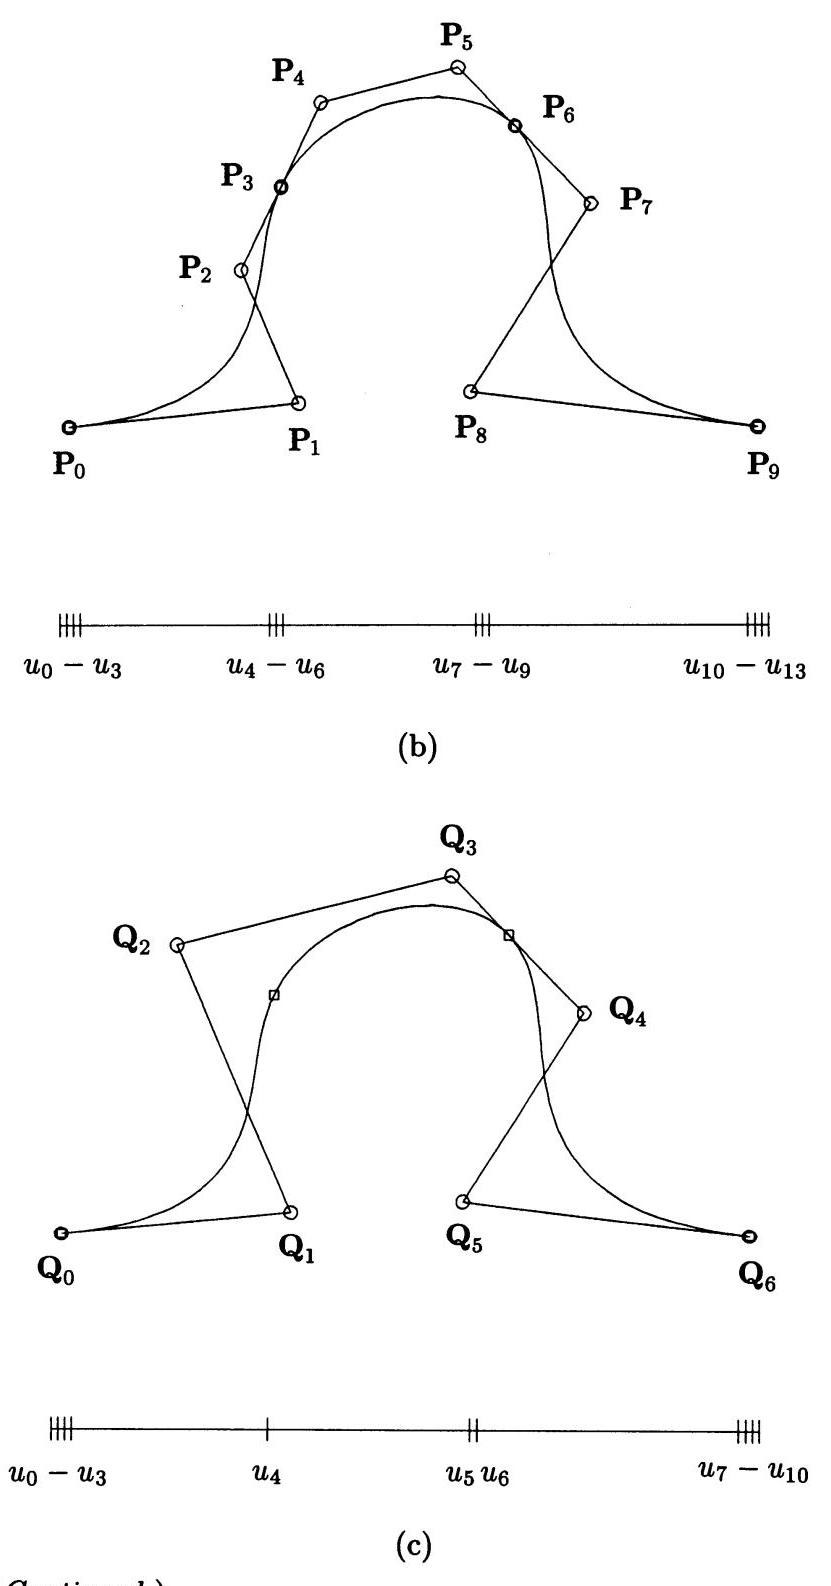
\includegraphics[max width=0.7\textwidth]{images/0193ba0d-ab19-7138-9798-cb281ce60de0_284_357_248_831_1586_0.jpg}
\end{center}
\hspace*{3em} 

图 6.20. (续)

算法 A6.2

PowerToBezierMatrix(p, M, MI)

\{ /* 计算 p 次贝塞尔矩阵的逆 */

/* 输入: p, M */

/* 输出: MI */

\HRule

for (i=0; i<p; i++) /* Set upper triangle to zero */

\hspace*{1em} for (j=i+1; j<=p; j++) MI[i][j] = 0.0;

/* Set first col, last row, and diagonal */

for (i = 0; i<=p; i++)

\hspace*{1em} \{

\hspace*{1em} MI[i][0] = MI[p][i] = 1.0;

\hspace*{1em} MI[i][i] = 1.0/M[i][i];

\hspace*{1em} \}

/* Compute remaining elements \(*\) /

\(\mathrm{k}1 = \left( {\mathrm{p} + 1}\right) /2;\;\mathrm{{pk}} = \mathrm{p} - 1;\)

for (k=1; k<k1; k++)

\hspace*{1em} \{

\hspace*{1em} for (j=k+1; j<=pk; j++)

\hspace*{3em} \{

\hspace*{3em} d = 0.0 ;

\hspace*{3em} for (i=k; i<j; i++) d = d-M[j][i]*MI[i][k];

\hspace*{3em} MI[j][k] = d/M[j][j];

\hspace*{3em} MI[pk][p-j] = MI[j][k];

\hspace*{3em} \}

\hspace*{1em} \(\mathrm{{pk}} = \mathrm{{pk}} - 1;\)

\hspace*{1em} \}

\}

\HRule

回顾公式 (6.85) 和 (6.86)，我们有 \(s = {cu} + d\) 和

\[
{\left\lbrack  {s}^{i}\right\rbrack  }^{T} = {\left\lbrack  {\left( cu + d\right) }^{i}\right\rbrack  }^{T} = {\left\lbrack  {u}^{i}\right\rbrack  }^{T}{R}_{p} \tag{6.97}
\]

反转公式 (6.85) 得到

\[
u = \frac{1}{c}s - \frac{d}{c} = \left( {{u}_{j + 1} - {u}_{j}}\right) s + {u}_{j} = {\gamma s} + \delta
\]

从公式 (6.97) 我们得到

\[
{\left\lbrack  {u}^{i}\right\rbrack  }^{T} = {\left\lbrack  {\left( \gamma s + \delta \right) }^{i}\right\rbrack  }^{T} = {\left\lbrack  {s}^{i}\right\rbrack  }^{T}{R}_{p}^{-1}
\]

这意味着 \({R}_{p}^{-1}\) 只是 \({R}_{p}\) ，其中 \(c\) 被 \(\gamma\) 替换， \(d\) 被 \(\delta\) 替换。总结来说

\[
{R}_{p}^{-1} = \left\lbrack  {r}_{i,j}\right\rbrack
\]

与

\[
{r}_{i,j} = \left\{  \begin{matrix} 0 & j < i \\  \left( \begin{matrix} j \\  i \end{matrix}\right) {\gamma }^{i}{\delta }^{j - i} & i \leq  j\;i,j = 0,\ldots ,p \end{matrix}\right.  \tag{6.98}
\]

其中

\[
\gamma  = {u}_{j + 1} - {u}_{j}\;\delta  = {u}_{j}
\]

我们总结了两点:

\begin{itemize}
\item 对于 IGES 参数样条， \(\delta  = 0\) 和 \({R}_{p}^{-1}\) 简化为对角矩阵 [IGE93]，其元素为
\end{itemize}

\[
{r}_{i,j} = \left\{  \begin{array}{ll} 0 & i \neq  j \\  {\gamma }^{i} & i = j\;i = 0,\ldots ,p \end{array}\right.  \tag{6.99}
\]

\begin{itemize}
\item 对于表面，方程 (6.93) 变为
\end{itemize}

\[
\left\lbrack  {\mathbf{P}}_{i,j}\right\rbrack   = {M}_{p}^{-1}{R}_{p}^{-1}\left\lbrack  {\mathbf{a}}_{i,j}\right\rbrack  {\left( {R}_{q}^{-1}\right) }^{T}{\left( {M}_{q}^{-1}\right) }^{T}
\]

其中 \({R}_{p}^{-1}\) 和 \({\left( {R}_{q}^{-1}\right) }^{T}\) 是重新参数化矩阵，将 \(s\) 转换为 \(u\) ，将 \(t\) 转换为 \(v\) ，分别 \(\left( {0 \leq  s,t \leq  1}\right)\) 。

图 \({6.21}\mathrm{a} - {6.21}\mathrm{c}\) 说明了从幂基到 NURBS 表面的转换。测试表面是九个度 \(\left( {3 \times  2}\right)\) 多项式片段的集合，如图 6.21a 所示。图 6.21b 说明了分段 Bézier 表示。去结点后产生的表面如图 6.21c 所示。

\begin{center}
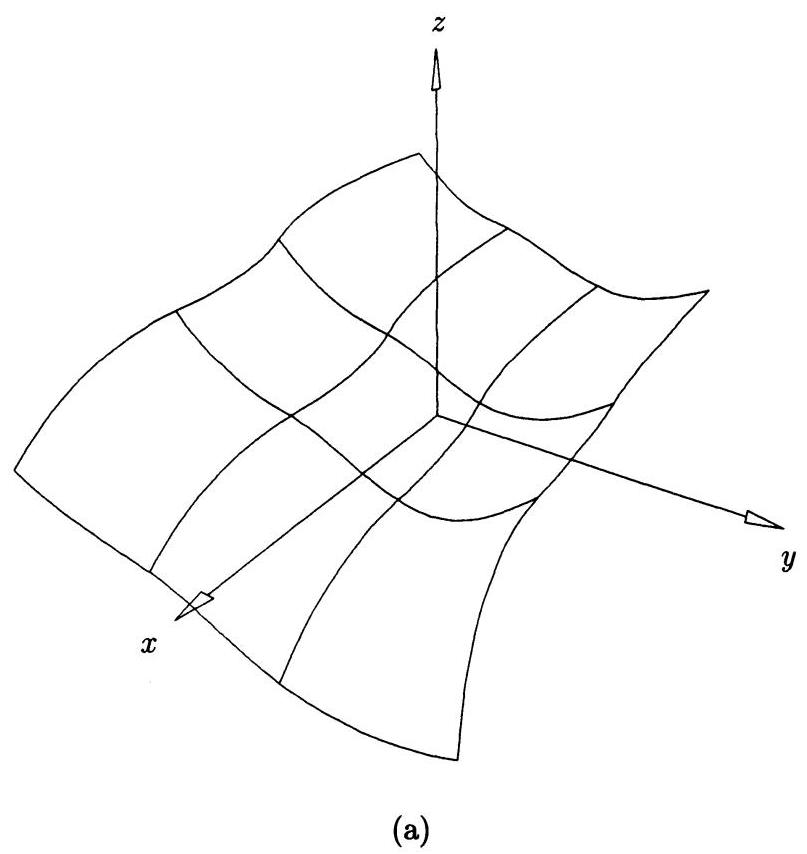
\includegraphics[max width=0.7\textwidth]{images/0193ba0d-ab19-7138-9798-cb281ce60de0_286_361_1132_807_854_0.jpg}
\end{center}
\hspace*{3em} 

图 6.21. 将分段多项式表面转换为 NURBS 形式。(a) 分段多项式表面；(b) 将每个片段转换为 Bézier 形式；(c) 去结点后的 NURBS 表示。

278 高级几何算法

\begin{center}
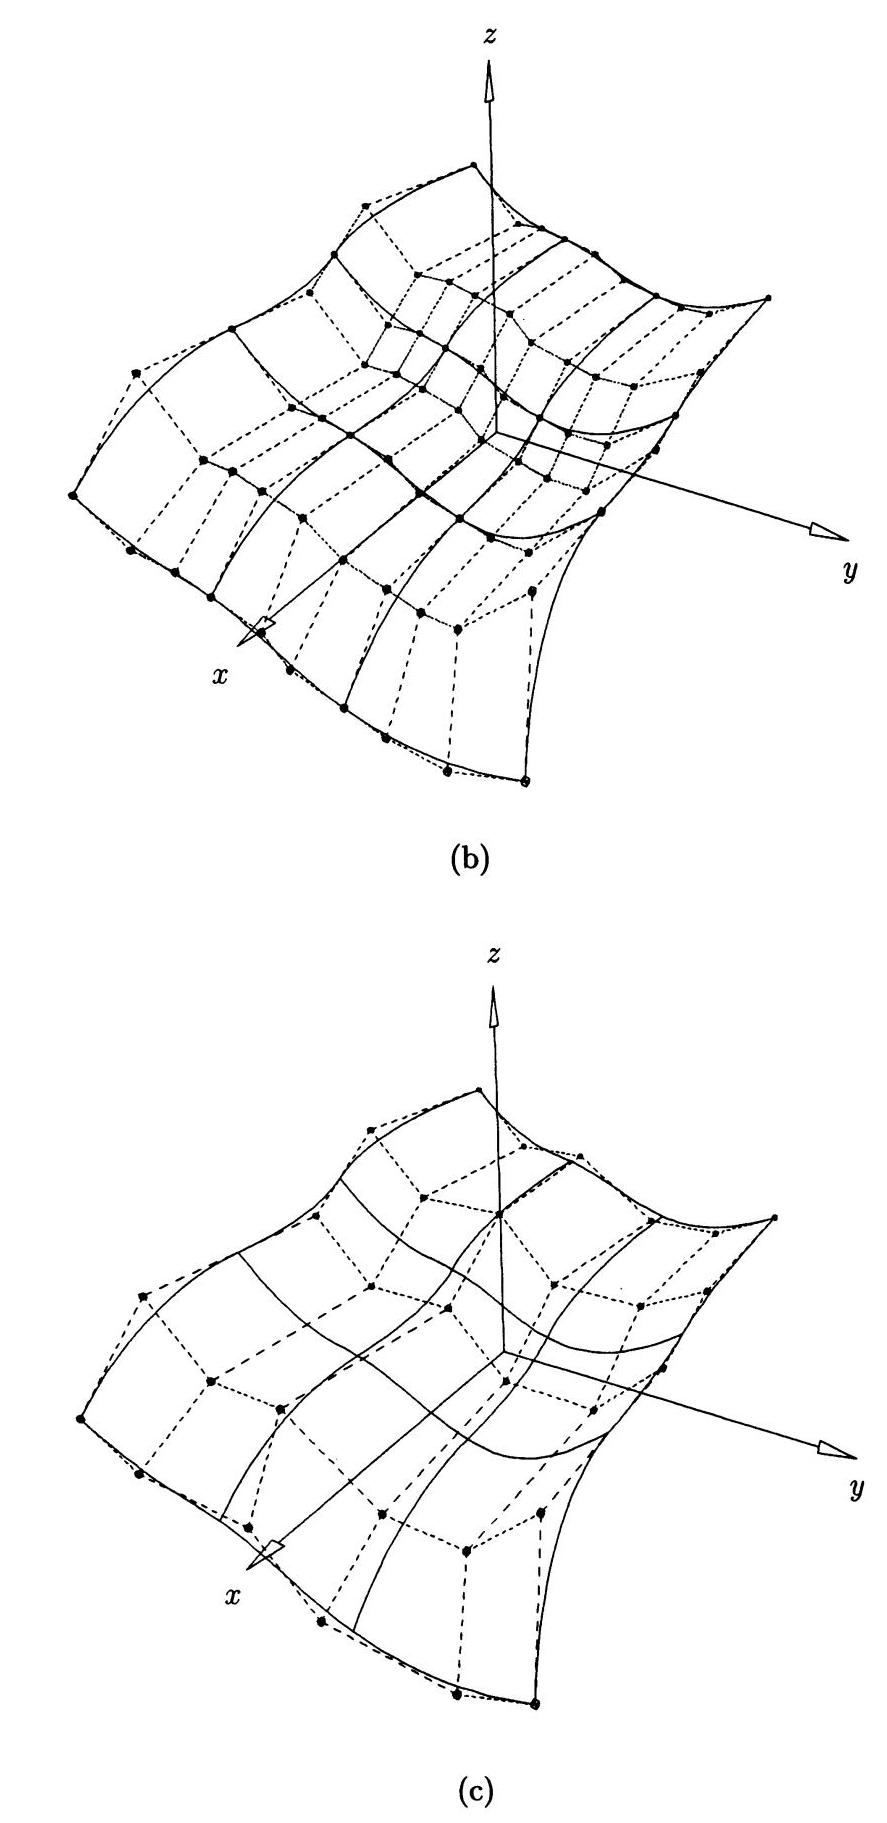
\includegraphics[max width=0.8\textwidth]{images/0193ba0d-ab19-7138-9798-cb281ce60de0_287_405_242_887_1823_0.jpg}
\end{center}
\hspace*{3em} 

图 6.21.(续)

\section*{练习}

6.1. 考虑示例 Ex6.3 的透视投影。 \({\overline{\mathbf{P}}}_{i}^{w}\) 的欧几里得坐标为

\[
{\overline{\mathbf{P}}}_{i} = \left( {\frac{d{x}_{i}}{d - {z}_{i}},\frac{d{y}_{i}}{d - {z}_{i}},0}\right)
\]

使用方程 (6.17) 和 (6.18) 进行投影；比较结果。

6.2. 使用二次函数 \(u = f\left( s\right)  = a{s}^{2} + {bs} + c\) 重新参数化由 \(\left\{  {\mathbf{P}}_{i}\right\}   = \{ \left( {1,0}\right) ,\left( {1,1}\right) ,\left( {0,1}\right) \}\) 和 \(\left\{  {w}_{i}\right\}   = \{ 1,1,2\}\) 给出的 Bézier 圆弧 \(\mathbf{C}\left( u\right)\) ，使得

\[
\mathbf{P} = \mathbf{C}\left( {s = \frac{1}{2}}\right)  = \left( {\frac{\sqrt{2}}{2},\frac{\sqrt{2}}{2}}\right)
\]

需要三个步骤:

\begin{itemize}
\item 确定 \(\mathbf{P}\) 达到的 \(u\) 值。提示:使用公式 (6.28)；
\end{itemize}

\begin{itemize}
\item 计算 \(f\left( s\right)\) 的系数 \(a,b,c\) ；
\end{itemize}

\begin{itemize}
\item 使用公式 (6.38) 确定新的齐次控制点。
\end{itemize}

末端权重是否发生了变化？

6.3. 在 \(U = \{ 0,0,0,0,1,1,3,5,7,7,7,7\}\) 上，使用非有理二次 NURBS 函数 \(f\left( s\right)\) 对立方曲线 \({\mathbf{C}}^{w}\left( u\right)\) 进行重新参数化 \(S = \{ 0,0,0,2,3,6,6,7,7,7\}\) 。重新参数化曲线 \({\mathbf{C}}^{w}\left( s\right)\) 的节点向量将是什么样的？在各个节点处 \({\mathbf{C}}^{w}\left( s\right)\) 的连续性如何？

6.4. 检查公式 (6.34) 与公式 (6.55)-(6.58) 之间的关系，即:

\begin{itemize}
\item 使用公式 (6.34)，公式 (6.56) 和公式 (6.57) 是否得出公式 (6.55)；
\end{itemize}

\begin{itemize}
\item 公式 (6.58) 是否产生公式 (6.34)？
\end{itemize}

请记住，所有权重都可以乘以一个共同因子。

6.5. 推导方程 (6.83)。

6.6. 设立立方曲线 \(\mathbf{C}\left( u\right)\) 由 \(U = \{ 0,0,0,0,1,2,2,2,2\}\) 定义，控制点为 \(\left\{  {\mathbf{P}}_{i}\right\}   = \{ \left( {0,0}\right) ,\left( {1,1}\right) ,\left( {3,2}\right) ,\left( {5,1}\right) ,\left( {4, - 1}\right) \}\) 。使用节点插入(手动)将曲线分解为两个贝塞尔段，然后将这两个段转换为幂基形式。通过从幂基段和原始 B-样条曲线计算一些端点和导数值来检查结果。

6.7. 设 \(s = {cu} + d\) 。形成 \({R}_{3}\) 和 \({R}_{3}^{-1}\) ，并验证 \({R}_{3}{R}_{3}^{-1} = I(I\) 是单位矩阵。



\clearpage

\end{document}


